\clearpage
\section{Data availability statement}

The original data presented in this chapter are openly available from the \texttt{GitHub} repository:
\href{https://github.com/Photonico/Graphene-BC_20230622}{\texttt{Photonico/Graphene-BC\_20230622}}.

\section{Supplementary information}
\label{1_supplementary}

The supplementary information presents the lattice-parameter determination for the graphene, borophene, \ce{BC3}, and \ce{B4C3} monolayers,
as well as the corresponding results for the associated heterostructure bilayers under various relative lateral displacements.
It also provides k-point mesh convergence tests, projected densities of states, dielectric function convergence tests, and derived optical properties for the monolayer and bilayer systems investigated.

\begin{figure}[!htbp]
\centering
    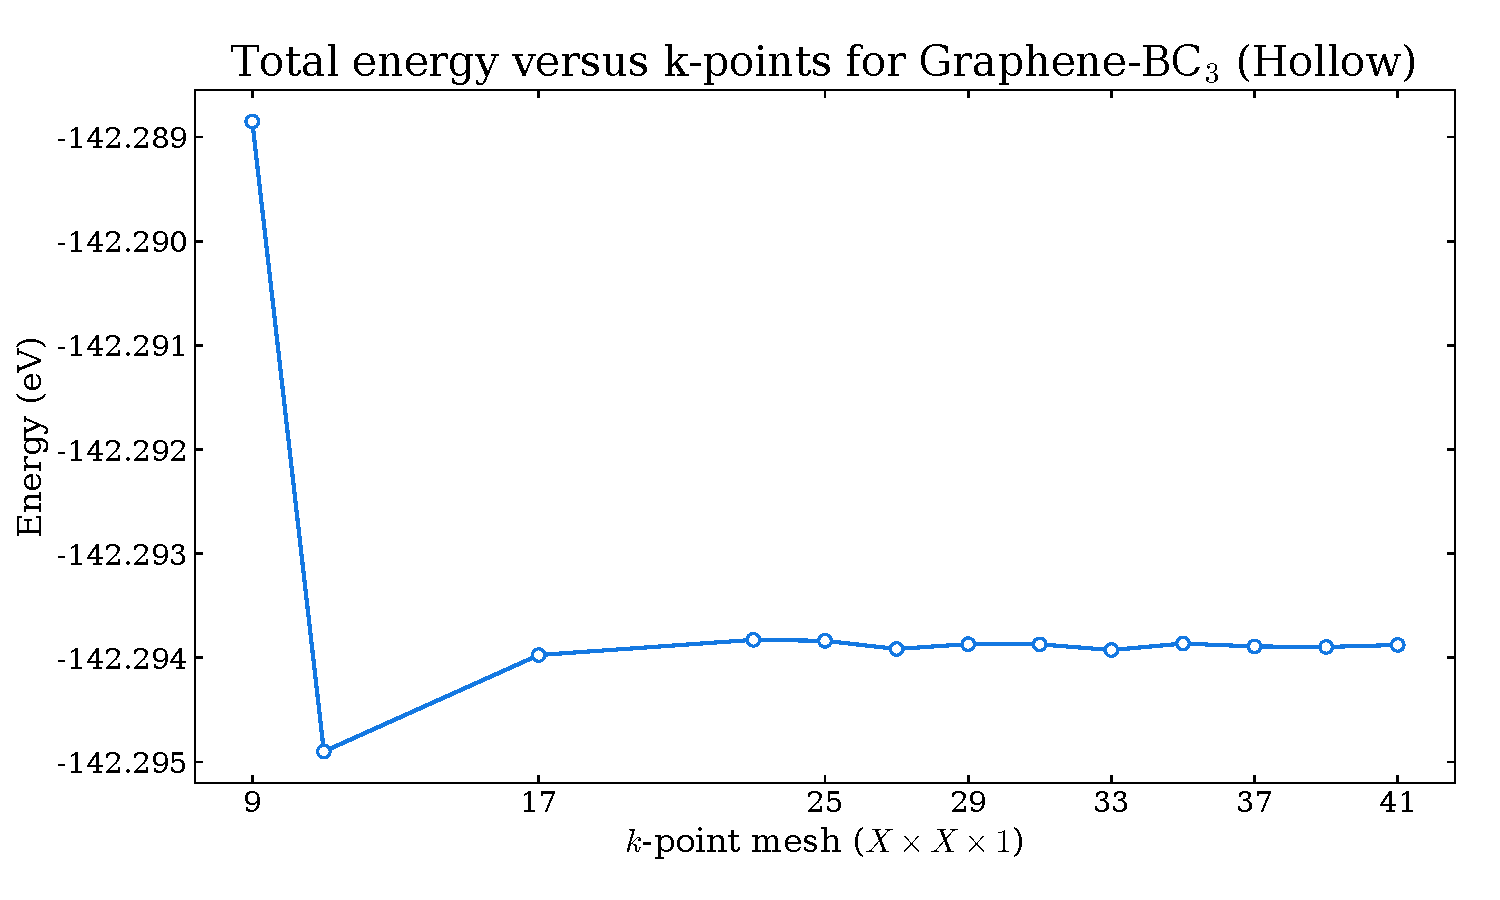
\includegraphics[width=0.60\textwidth]{figures_proj1/S1.1.pdf}
    \caption{Total energy versus the k-point mesh used to sample the Brillouin zone for the Graphene-\ce{BC3} bilayer; here, $\mathrm{X}$ denotes an $\mathrm{X} \times \mathrm{X} \times 1$~k-point mesh.}
\label{S1.1}
\end{figure}

\begin{figure}[!htbp]
\centering
    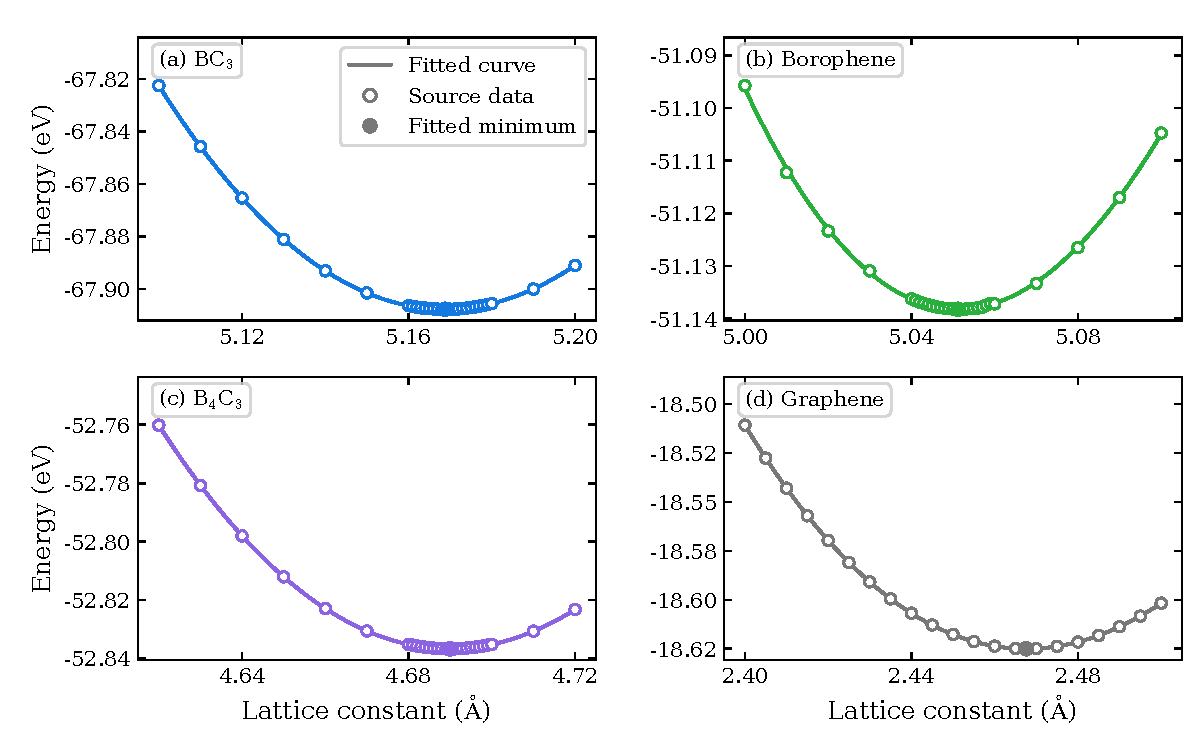
\includegraphics[width=0.80\textwidth]{figures_proj1/S1.2.pdf}
\caption{Total energy versus lattice constant for (a) \ce{BC3}, (b) borophene, (c) \ce{B4C3}, and (d) graphene.
The lattice constant yielding the lowest total energy is shown by the full circle in each plot.}
\label{S1.2}
\end{figure}

\begin{figure}[!htbp]
\centering
    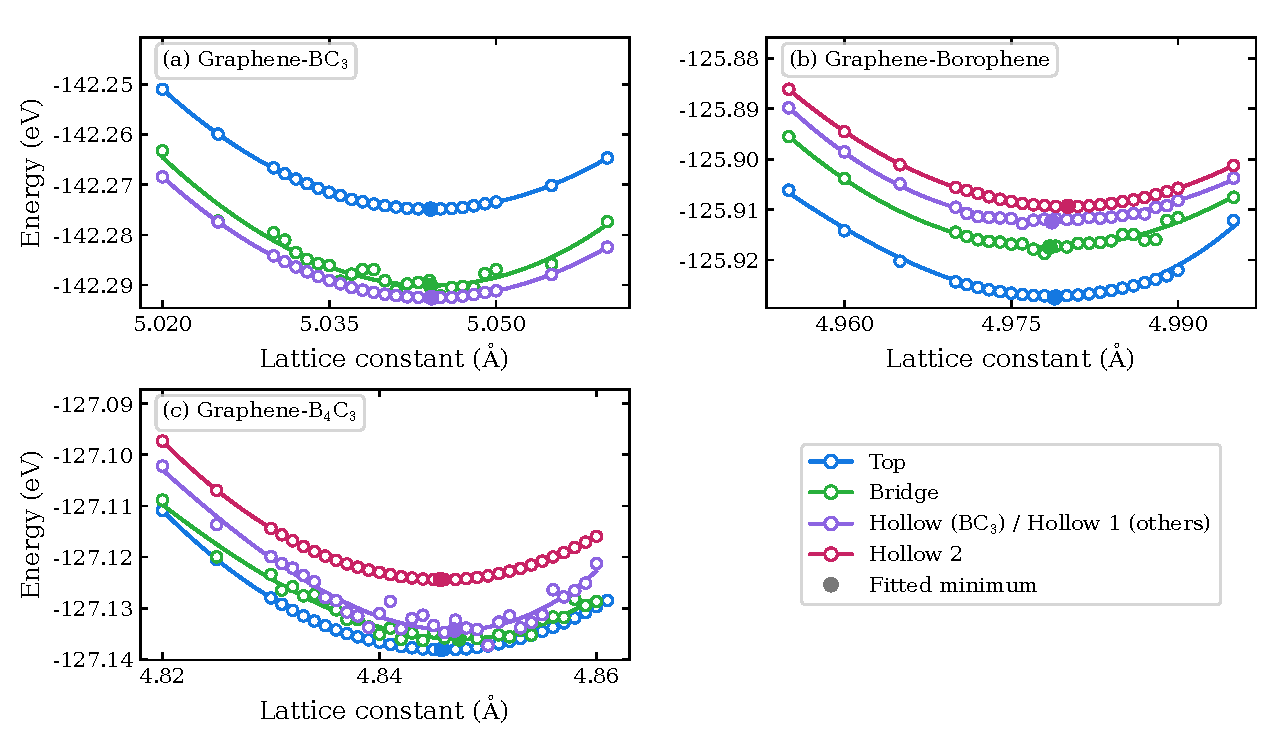
\includegraphics[width=0.80\textwidth]{figures_proj1/S1.3.pdf}
\caption{Total energy versus lattice constant for each bilayer system for the various stacking positions considered.
The lines are fitted curves, with the full circle indicating the lowest-energy structure.}
\label{S1.3}
\end{figure}

Figures~\ref{S1.4}--\ref{S1.6} show the total energy versus the lattice constant and interlayer distance for the various lateral positions considered.
The horizontal and vertical axes give the lattice constant and interlayer spacing, respectively, both in \si{\angstrom}; the colour scale gives the total energy in \unit{\electronvolt}.
The marker in each panel identifies the lowest-energy sampled geometry; the colour field interpolates the sampled energies.
These sampled minima are distinct from the relaxed structural parameters listed in table~\ref{tab:1.2_heterostructure}.

\begin{figure}[!htbp]
\centering
    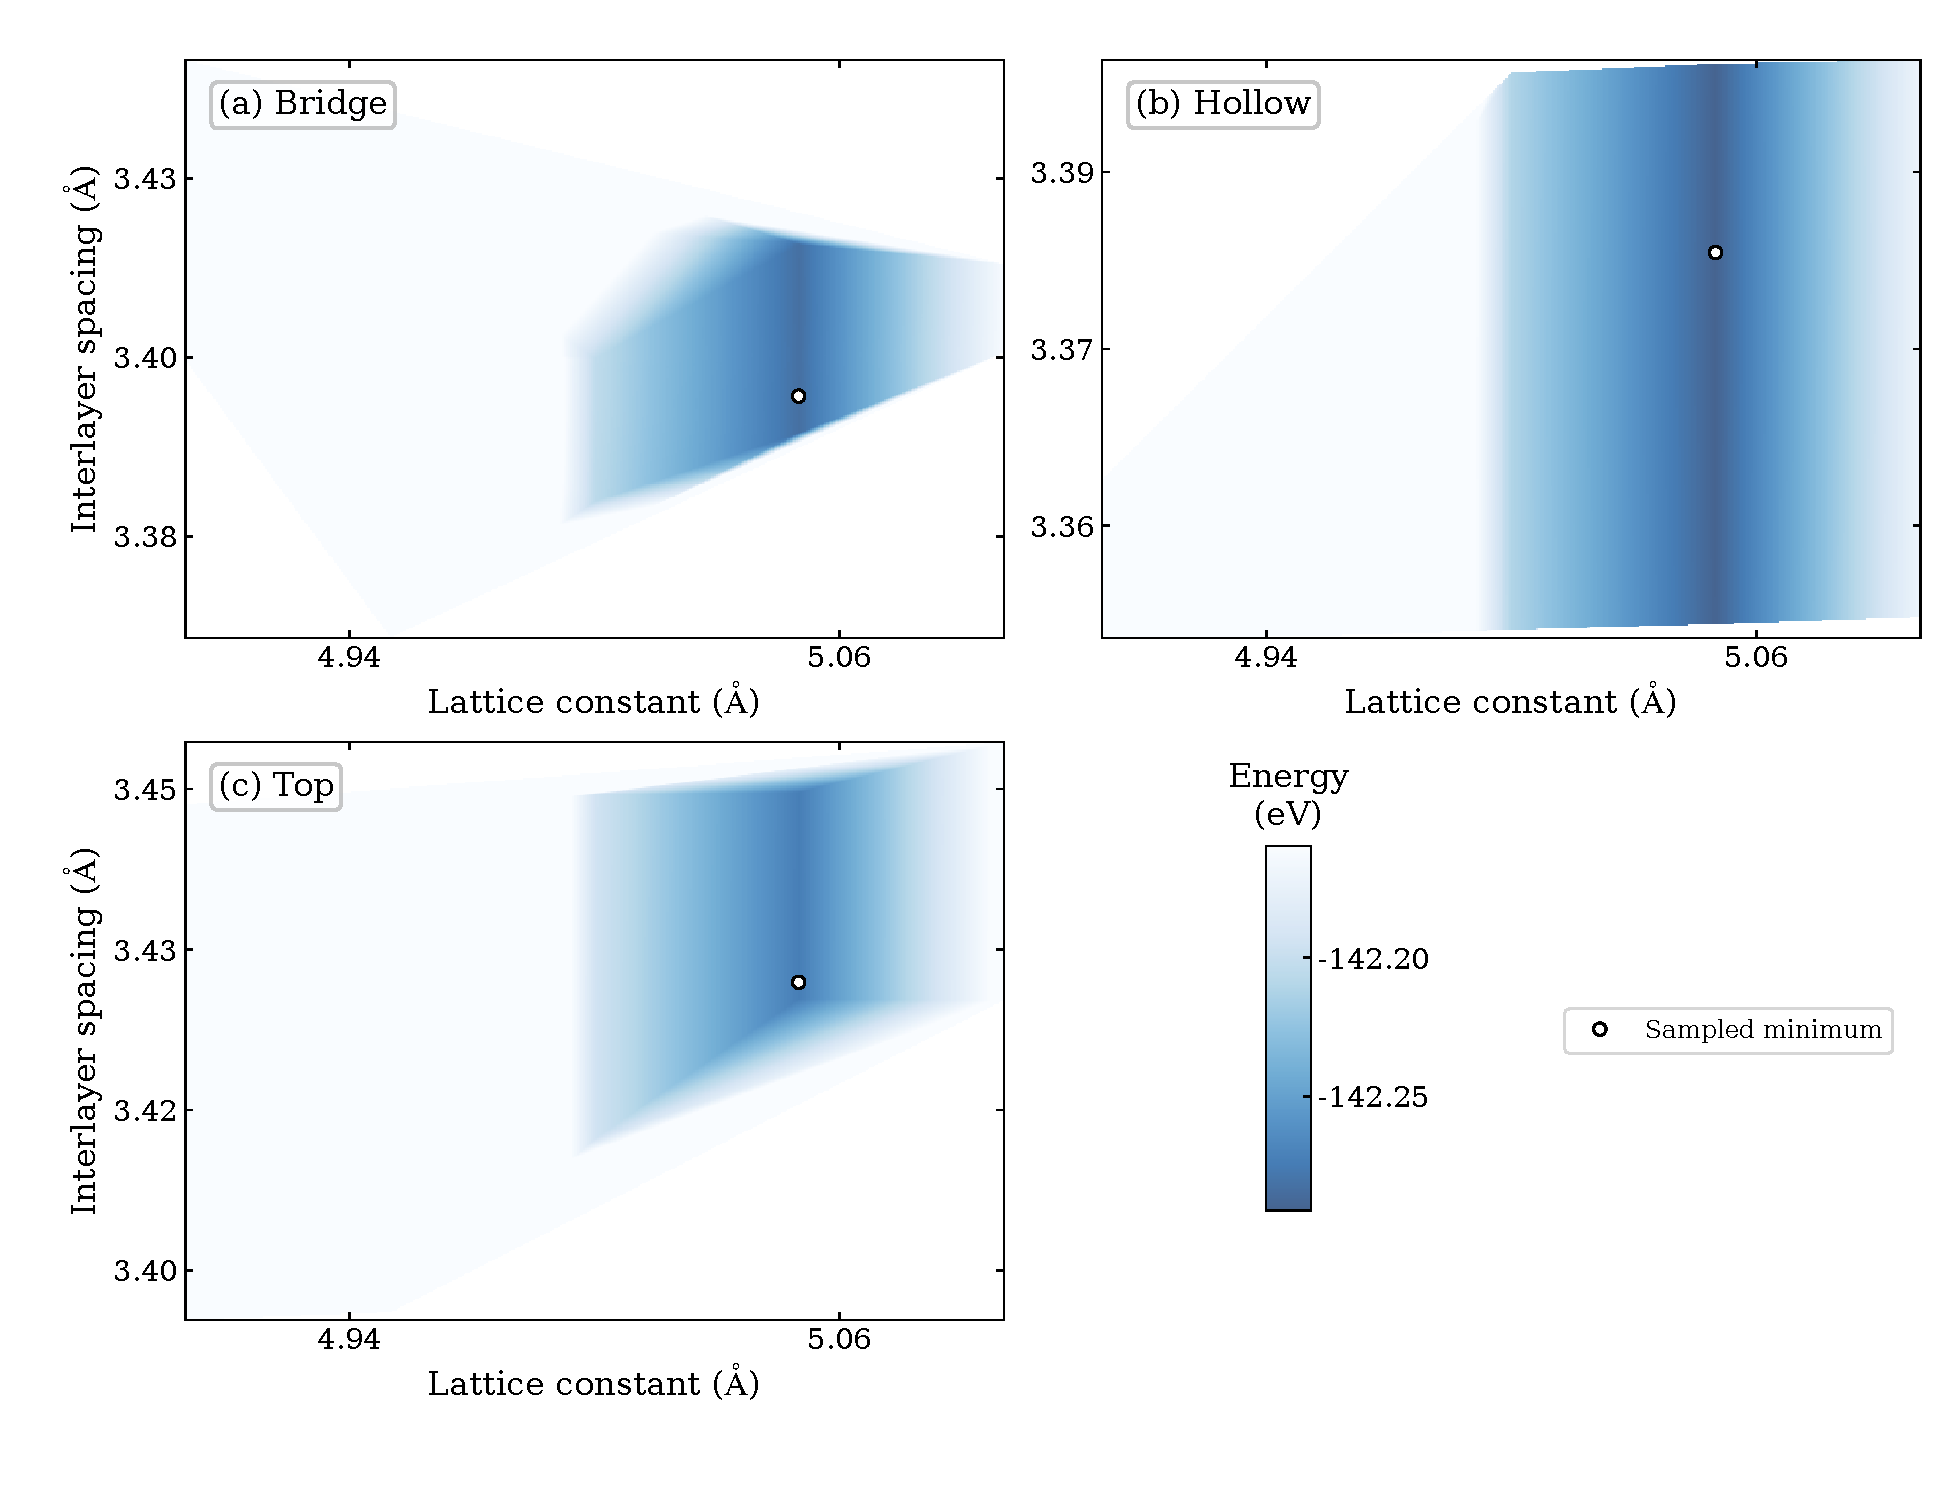
\includegraphics[width=0.80\textwidth]{figures_proj1/S1.4.pdf}
\caption{Total-energy landscape of the Graphene-\ce{BC3} bilayer.}
\label{S1.4}
\end{figure}


\begin{figure}[!htbp]
\centering
    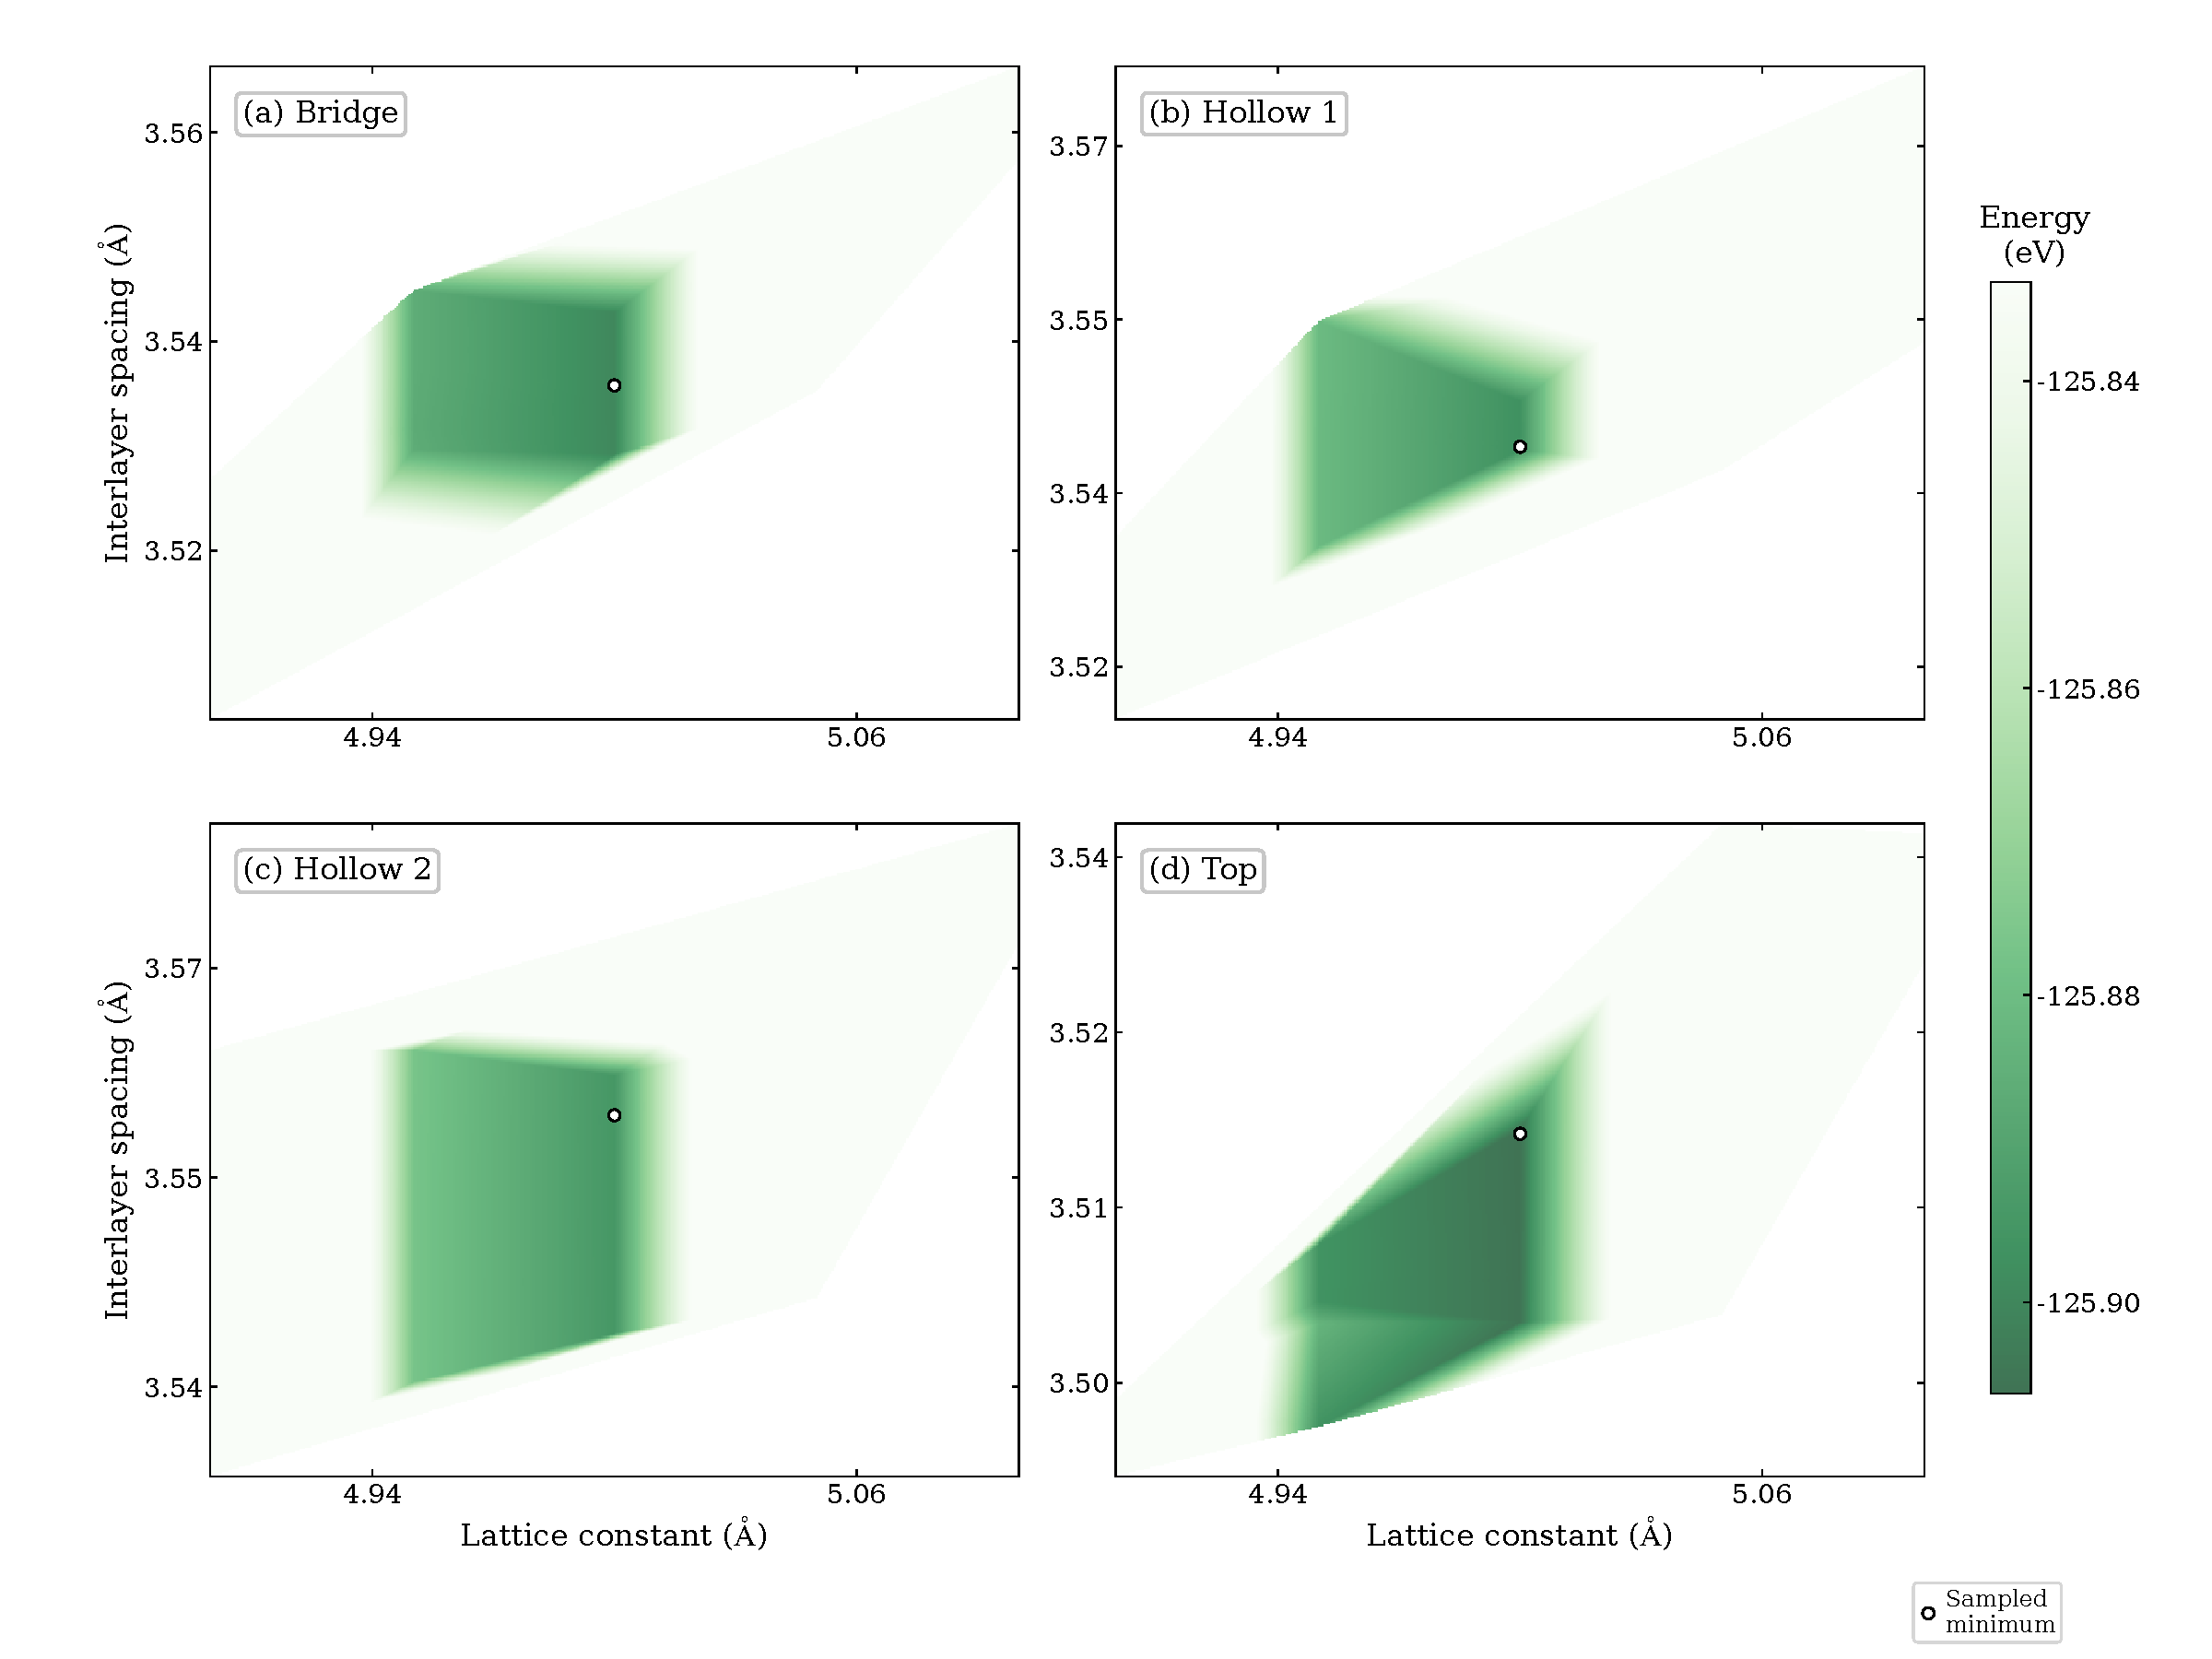
\includegraphics[width=0.80\textwidth]{figures_proj1/S1.5.pdf}
\caption{Total-energy landscape of the Graphene-Borophene bilayer.}
\label{S1.5}
\end{figure}


\begin{figure}[!htbp]
\centering
    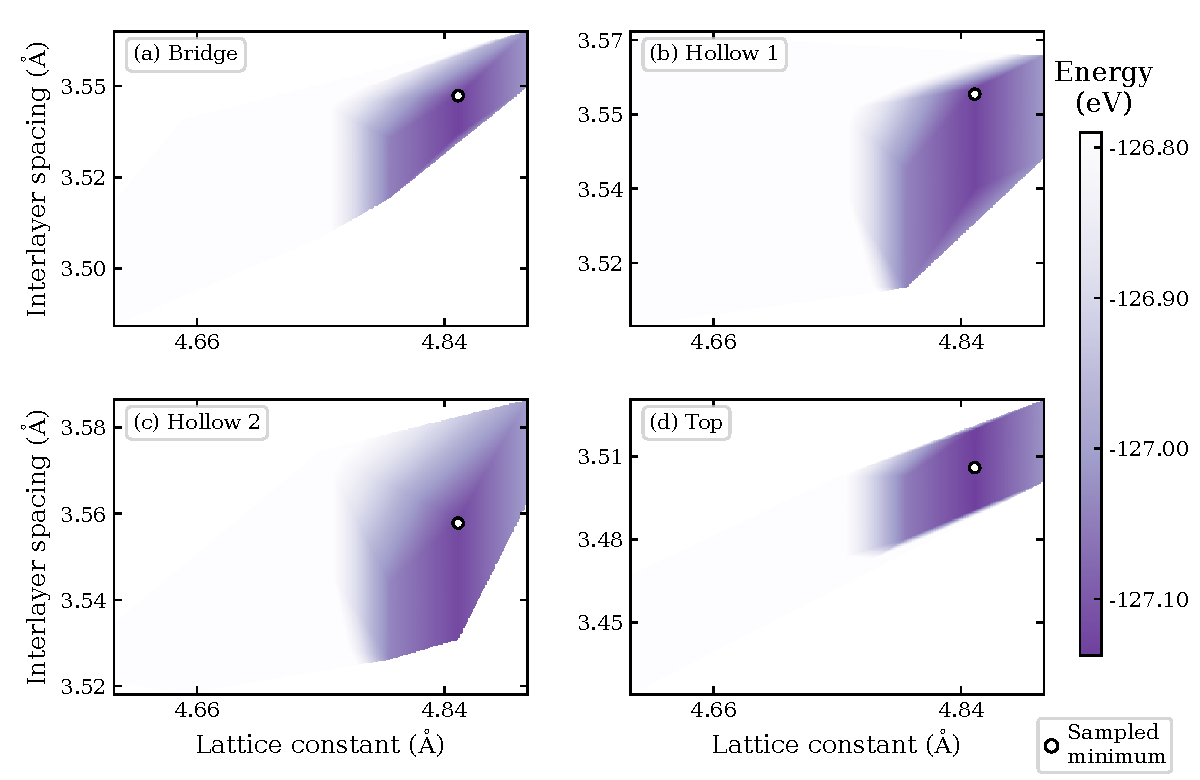
\includegraphics[width=0.80\textwidth]{figures_proj1/S1.6.pdf}
\caption{Total-energy landscape of the Graphene-\ce{B4C3} bilayer.}
\label{S1.6}
\end{figure}


\begin{table}[!htbp]
\centering
\begin{adjustbox}{max width=1.0\linewidth}
\begin{tabular}{cccccc}
\hline
\rowcolor{gray!25}
system
& site
& lattice constant (Å)
& interlayer spacing (Å)
& total energy (eV)
& relative energy (eV) \\ \hline

\multirow{3}{*}{Graphene-\ce{BC3}}
& Top
& 5.044
& 3.432
& -142.275
& 0.018 \\

& \cellcolor{gray!15} Bridge
& \cellcolor{gray!15} 5.044
& \cellcolor{gray!15} 3.384
& \cellcolor{gray!15} -142.290
& \cellcolor{gray!15} 0.002 \\

& \textbf{Hollow}
& \textbf{5.044}
& \textbf{3.375}
& \textbf{-142.293}
& \textbf{0.000} \\ \hline

\rowcolor{gray!15}
% \cellcolor{white}
\cellcolor{gray!15}
& \textbf{Top}
& \textbf{4.979}
& \textbf{3.496}
& \textbf{-125.927}
& \textbf{0.000} \\

% \cellcolor{white}
\cellcolor{gray!15}
& Bridge
& 4.979
& 3.505
& -125.921
& 0.006 \\

\rowcolor{gray!15}
% \cellcolor{white}
\cellcolor{gray!15}
& Hollow 1
& 4.979
& 3.551
& -125.914
& 0.013 \\

% \cellcolor{white}
\cellcolor{gray!15}
\multirow{-4}{*}{Graphene-Borophene}
& Hollow 2
& 4.979
& 3.548
& -125.909
& 0.018 \\ \hline

\rowcolor{gray!15}
\cellcolor{white}
& \textbf{Top}
& \textbf{4.846}
& \textbf{3.514}
& \textbf{-127.138}
& \textbf{0.000} \\

\cellcolor{white}
& Bridge
& 4.846
& 3.536
& -127.135
& 0.003 \\

\rowcolor{gray!15}
\cellcolor{white}
& Hollow 1
& 4.846
& 3.545
& -127.133
& 0.005 \\

\cellcolor{white}
\multirow{-4}{*}{Graphene-\ce{B4C3}}
& Hollow 2
& 4.846
& 3.562
& -127.124
& 0.014 \\ \hline

\end{tabular}
\end{adjustbox}
\caption{For each bilayer system and each lateral position considered, the optimized lattice constant, interlayer spacing, total energy, and relative energy are given.
The relative energy is given with respect to the most favourable structure, which corresponds to the lowest total energy for each bilayer system.}
\label{tab:S1.1}
\end{table}

\clearpage
In addition, figures~\ref{S1.9}--\ref{S1.11} show the projected densities of states of the three heterostructure systems calculated using the HSE06 functional.

\begin{figure}[!htbp]
\centering
    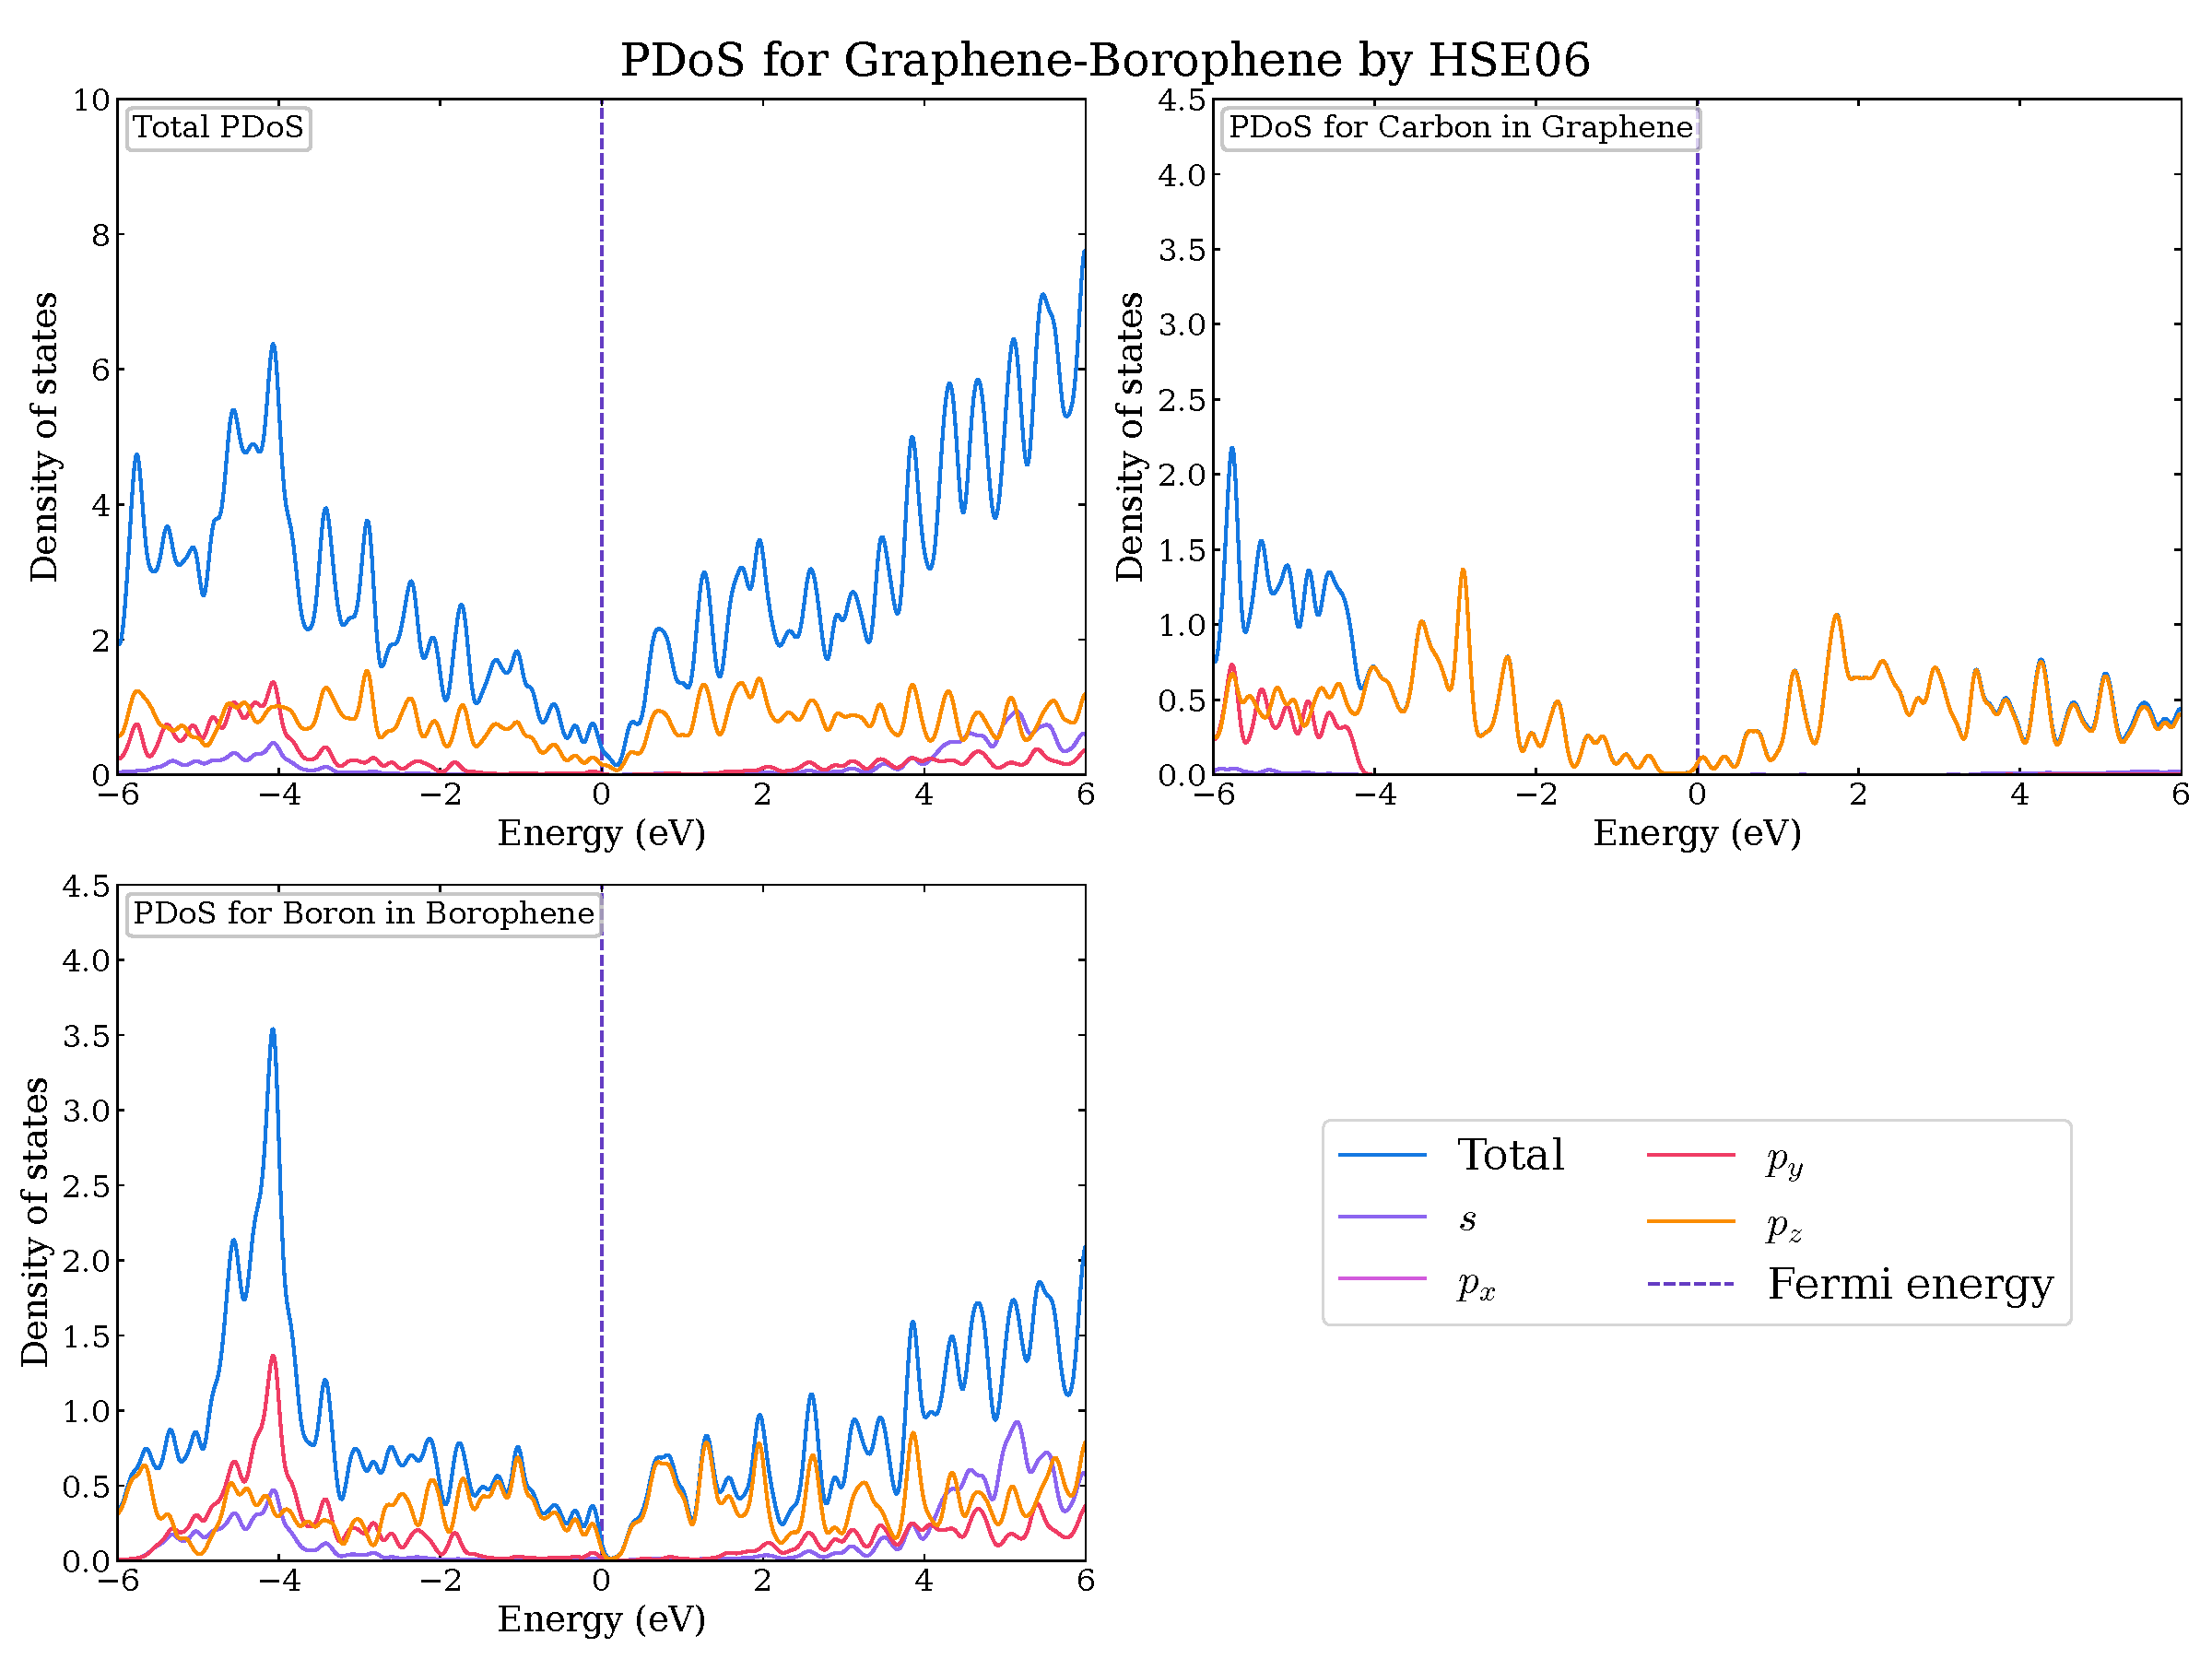
\includegraphics[width=0.80\textwidth]{figures_proj1/S1.9.pdf}
\caption{Projected density of states of Graphene-Borophene calculated using the HSE06 functional.}
\label{S1.9}
\end{figure}

\begin{figure}[!htbp]
\centering
    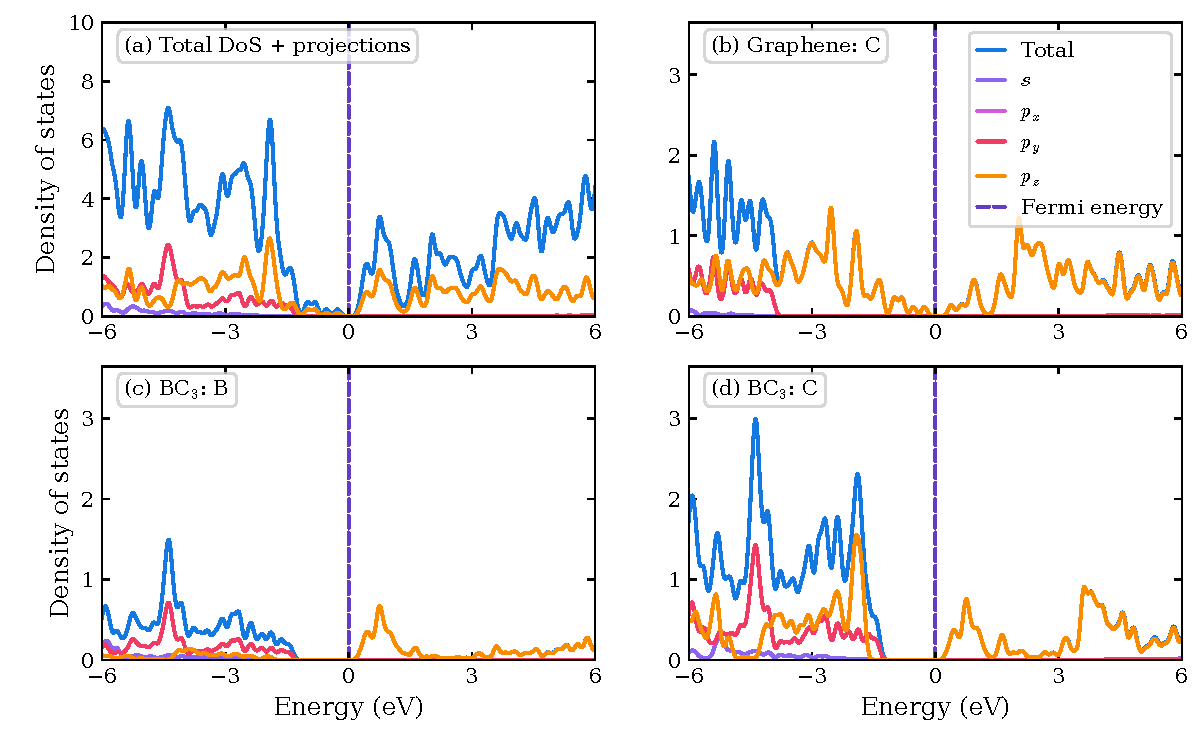
\includegraphics[width=0.80\textwidth]{figures_proj1/S1.10.pdf}
\caption{Projected density of states of the Graphene-\ce{BC3} calculated using the HSE06 functional.}
\label{S1.10}
\end{figure}

\begin{figure}[!htbp]
\centering
    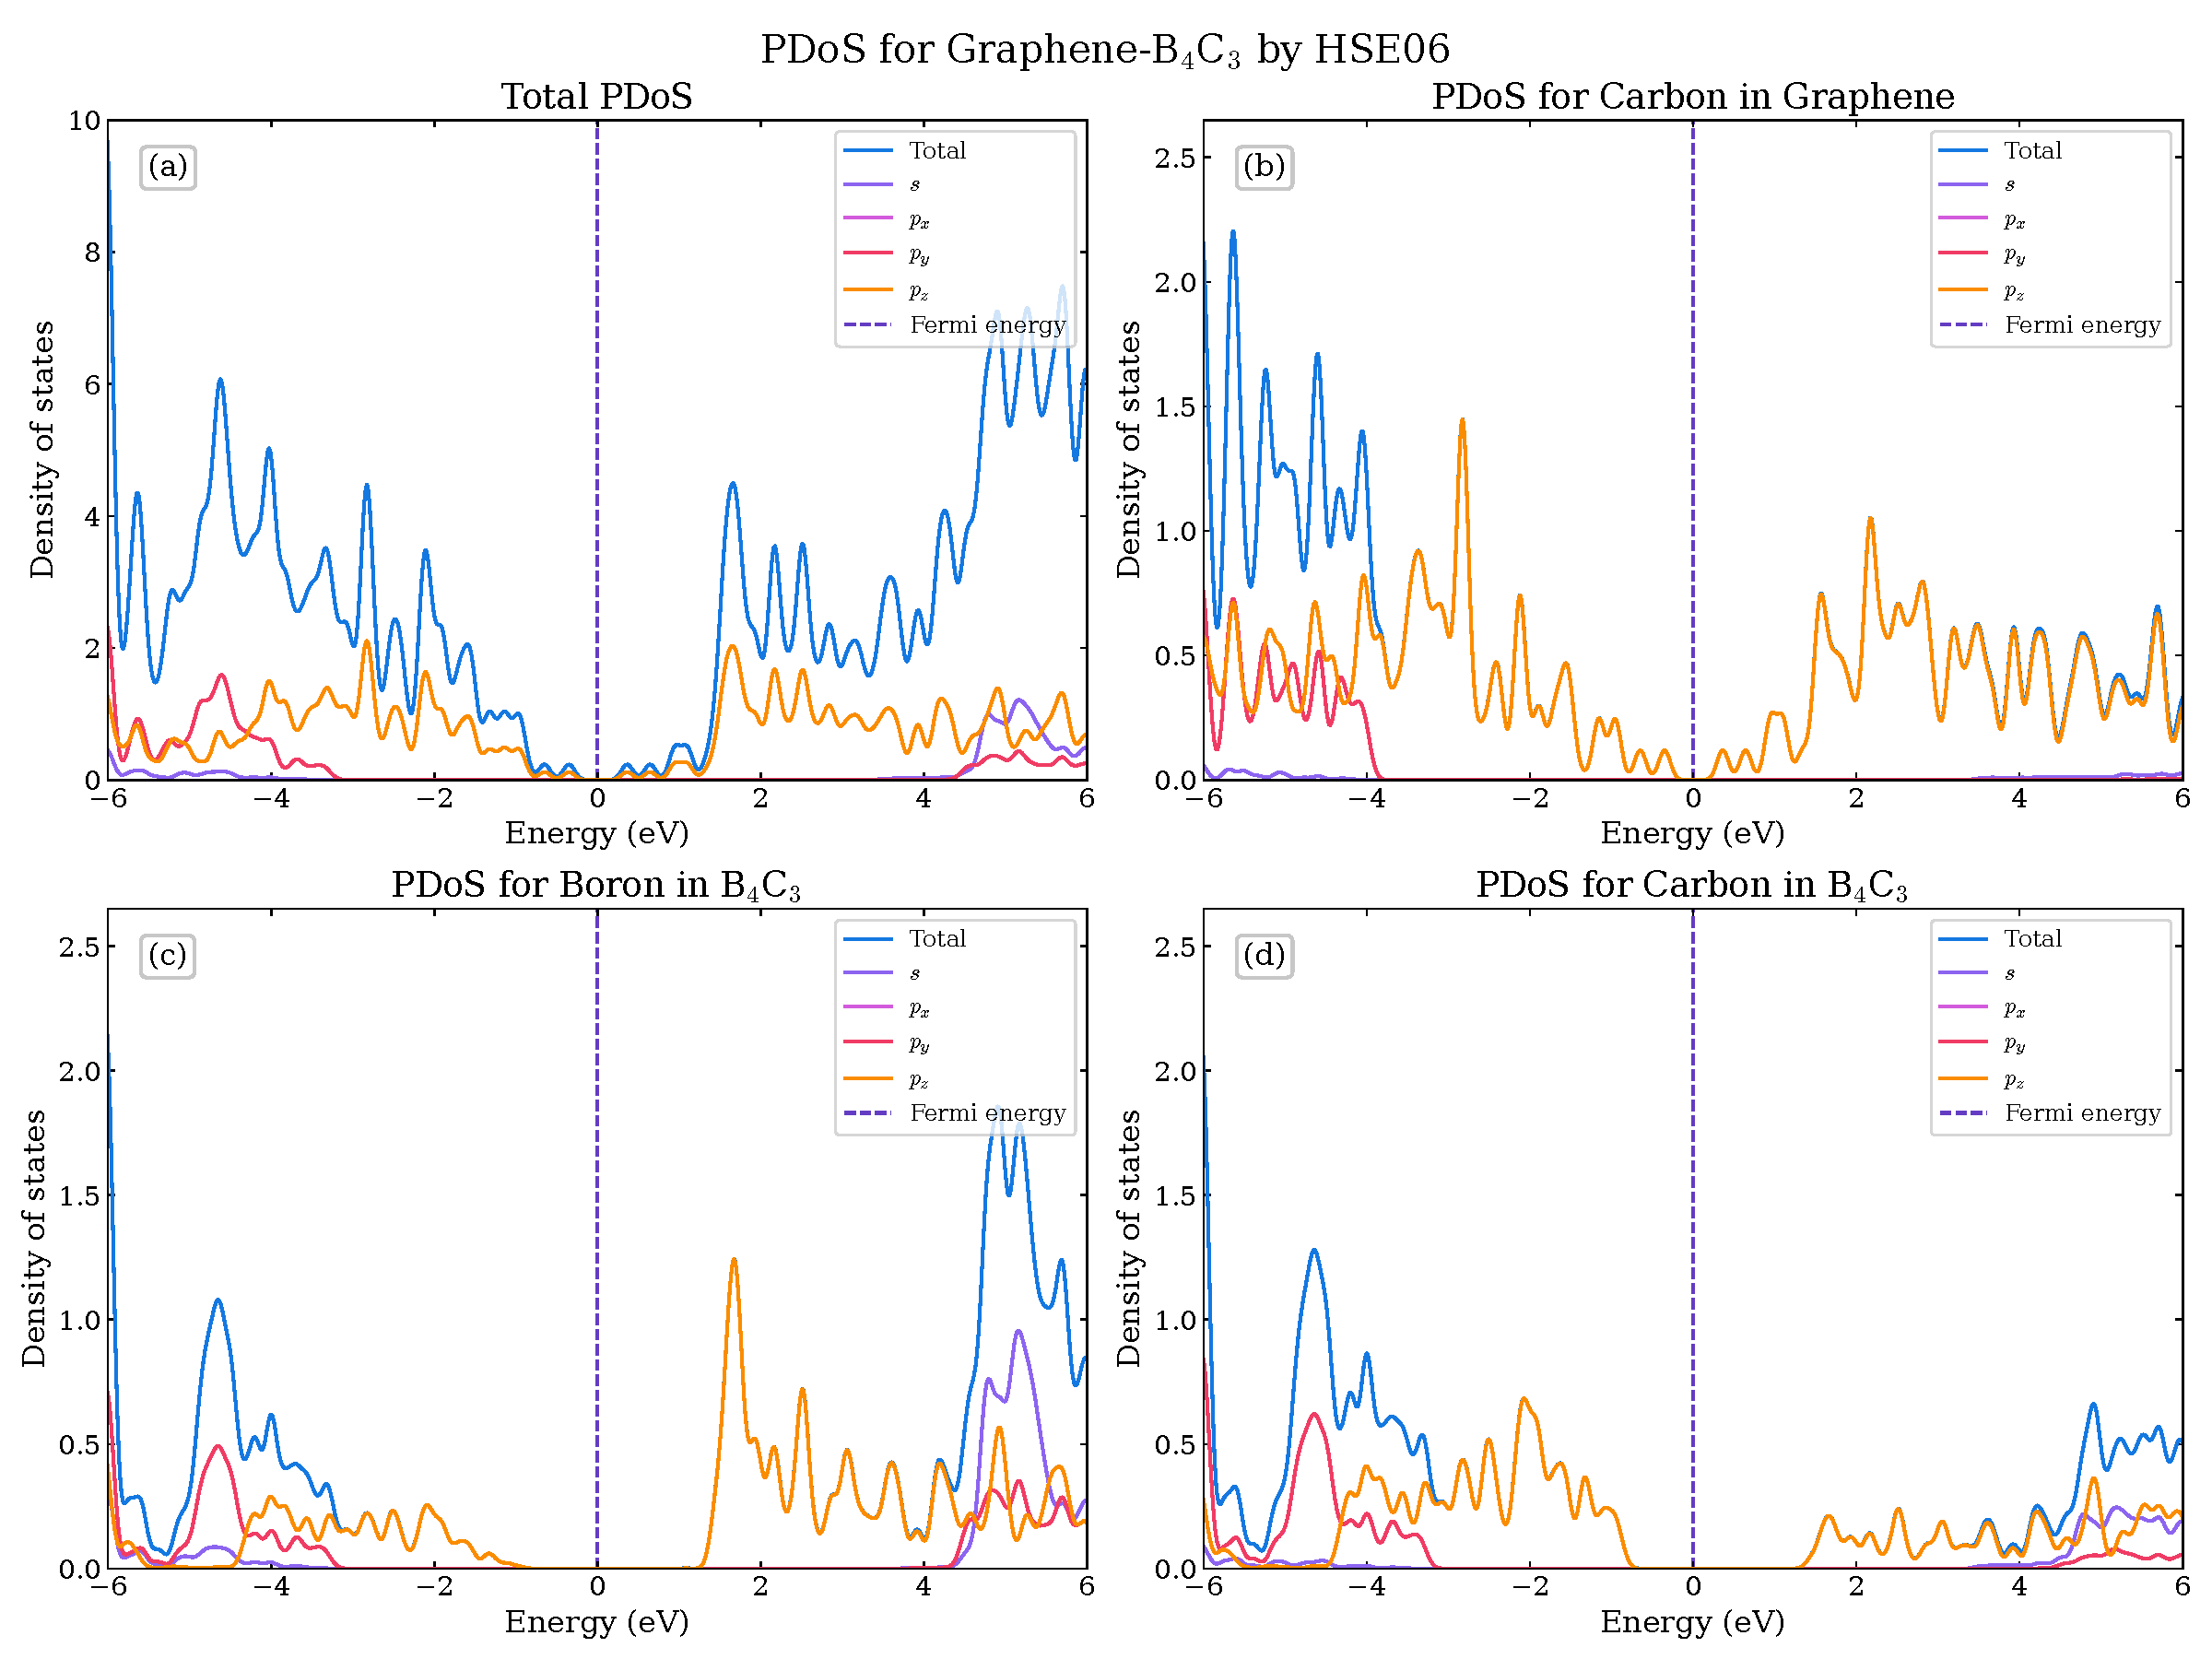
\includegraphics[width=0.80\textwidth]{figures_proj1/S1.11.pdf}
\caption{Projected density of states of the Graphene-\ce{B4C3} calculated using the HSE06 functional.}
\label{S1.11}
\end{figure}

\begin{figure}[!htbp]
\centering
    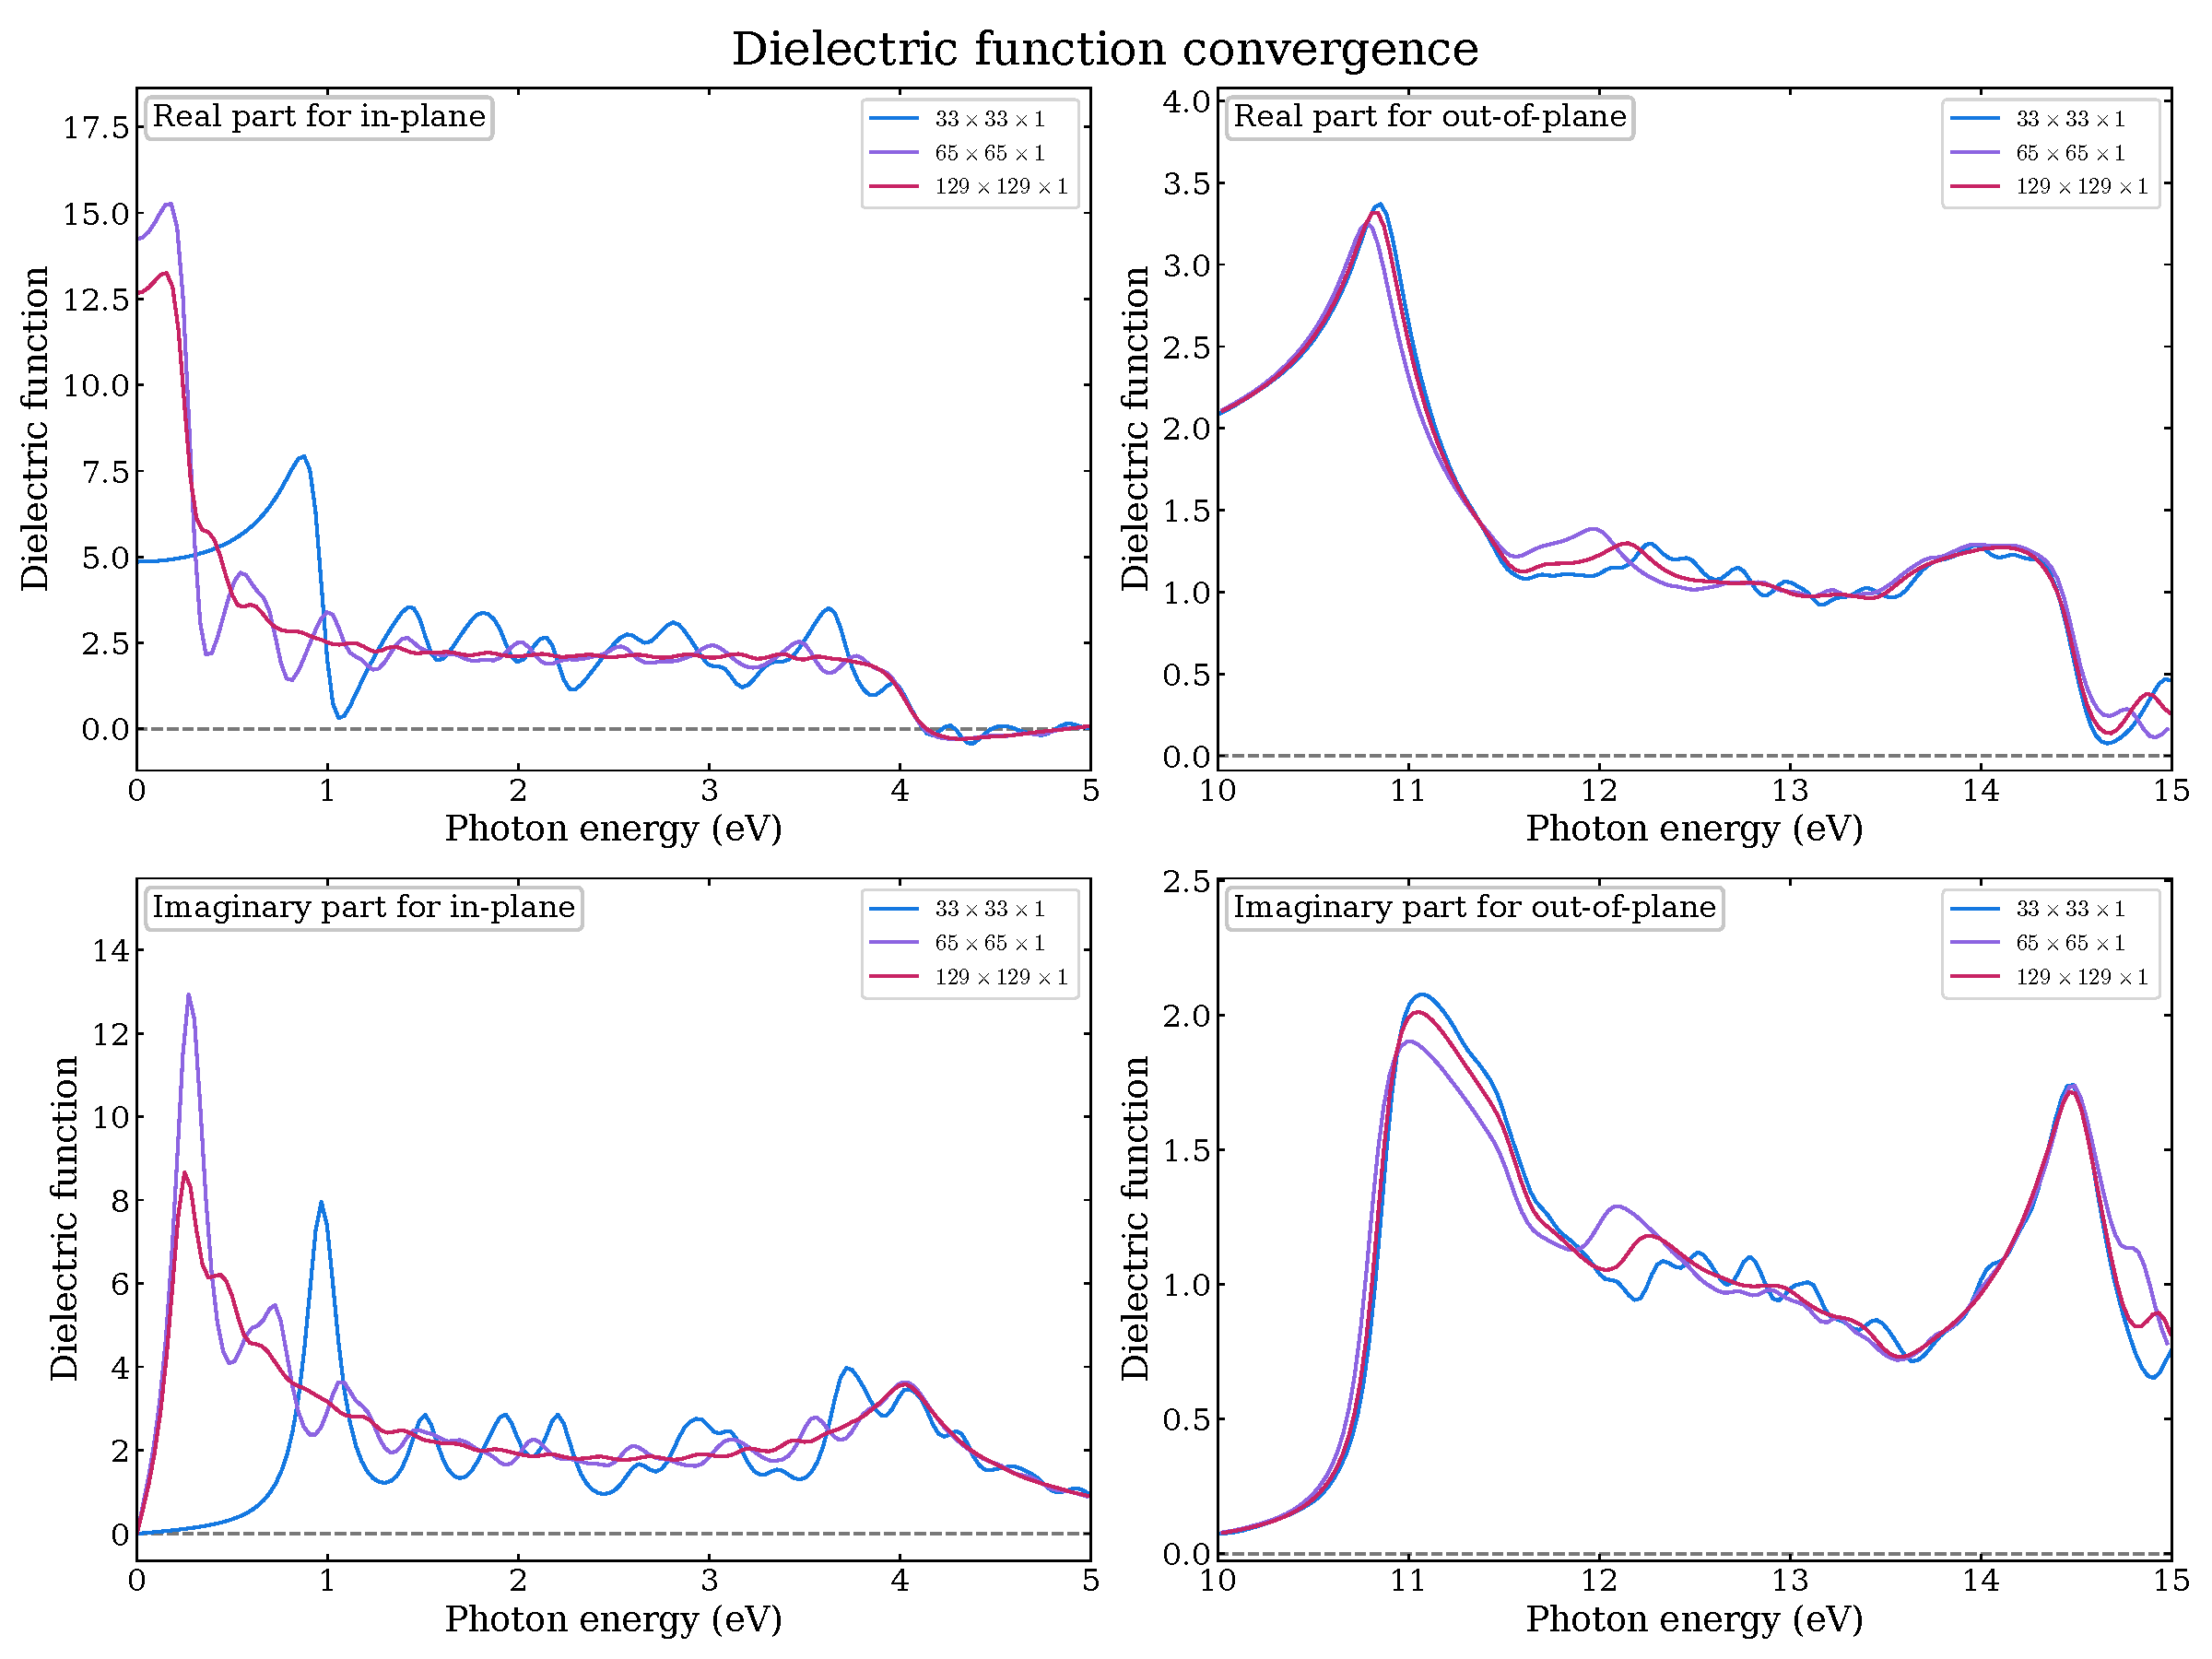
\includegraphics[width=0.80\textwidth]{figures_proj1/S1.12_alt.pdf}
\caption{Dielectric function of graphene calculated using the PBE functional for different k-point meshes;
here, for example,
$33$ denotes a $33 \times 33 \times 1$ k-point mesh.}
\label{S1.12}
\end{figure}

\begin{figure}[!htbp]
\centering
    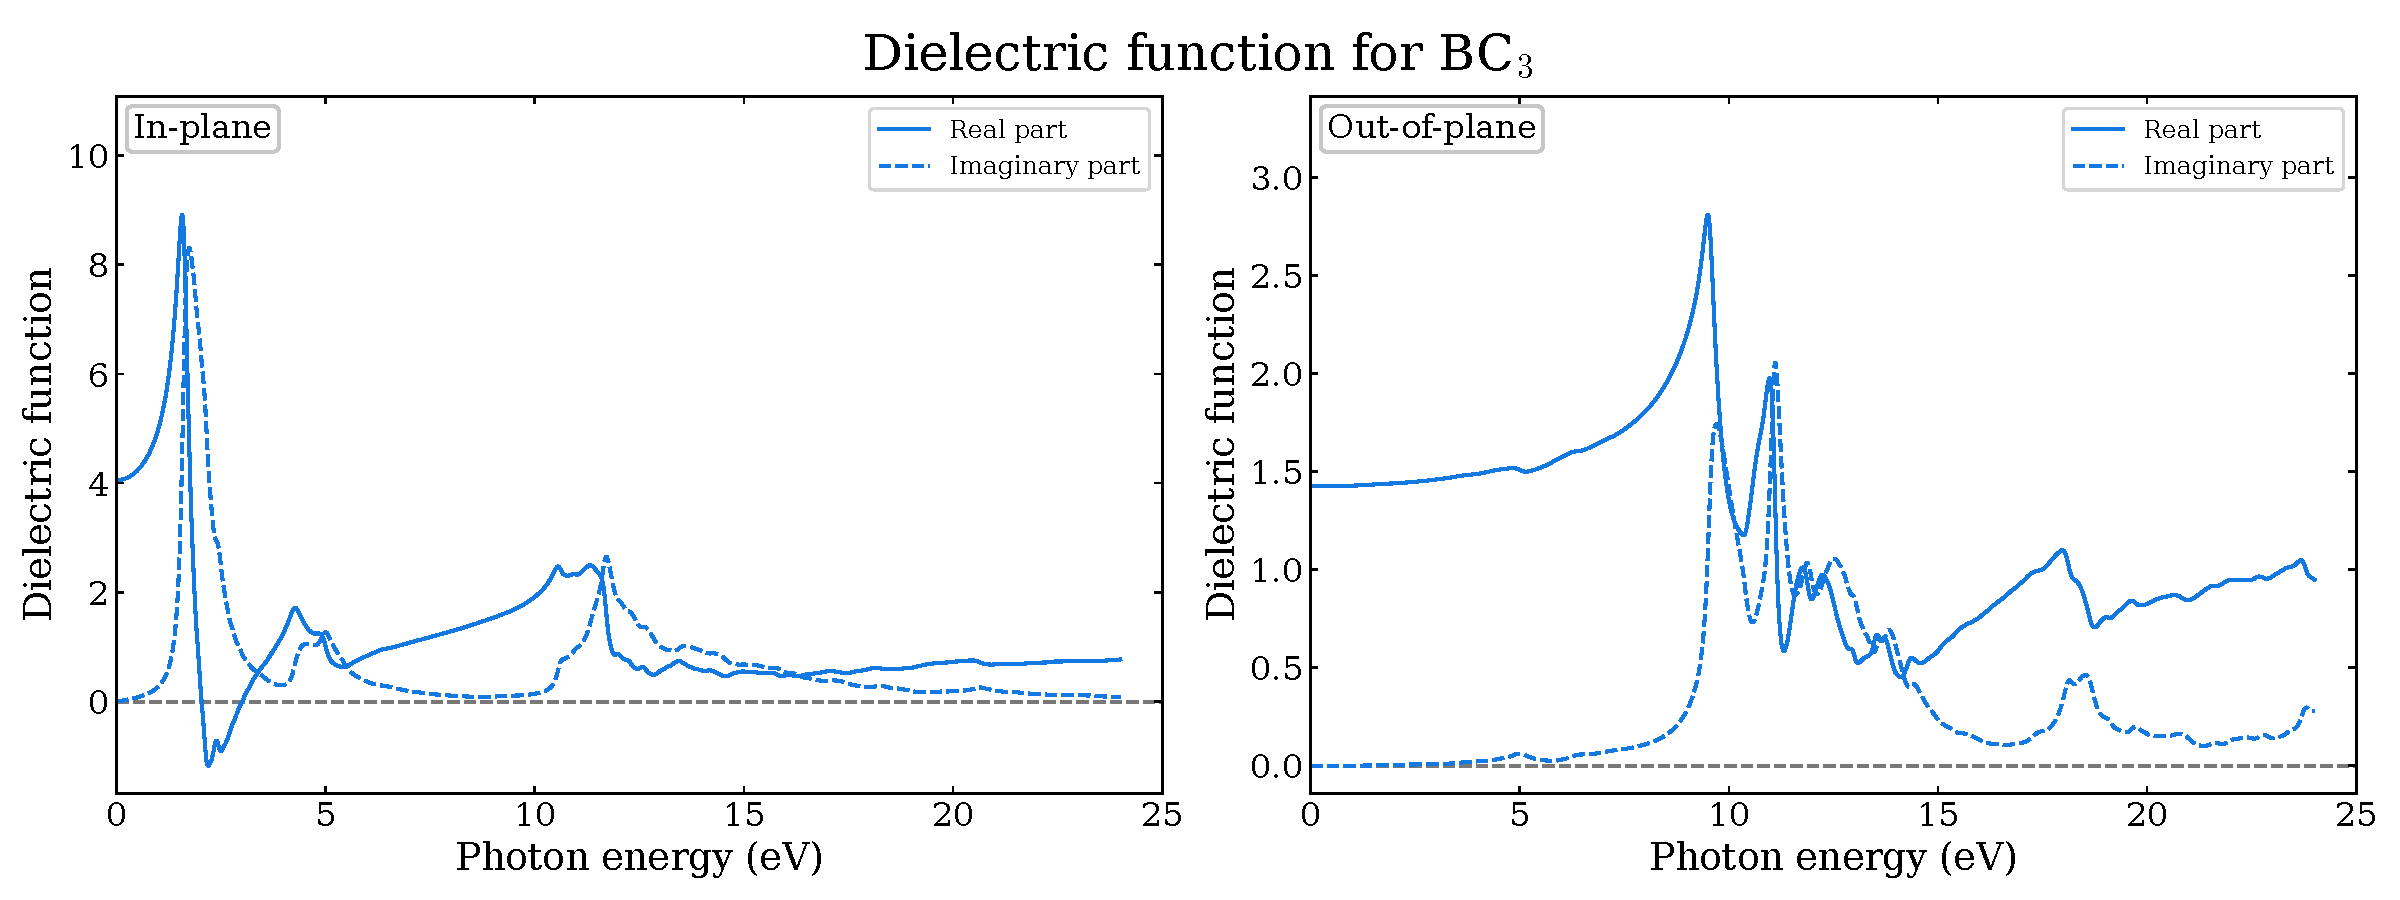
\includegraphics[width=0.80\textwidth]{figures_proj1/S1.13a.pdf}
    \par\nointerlineskip
    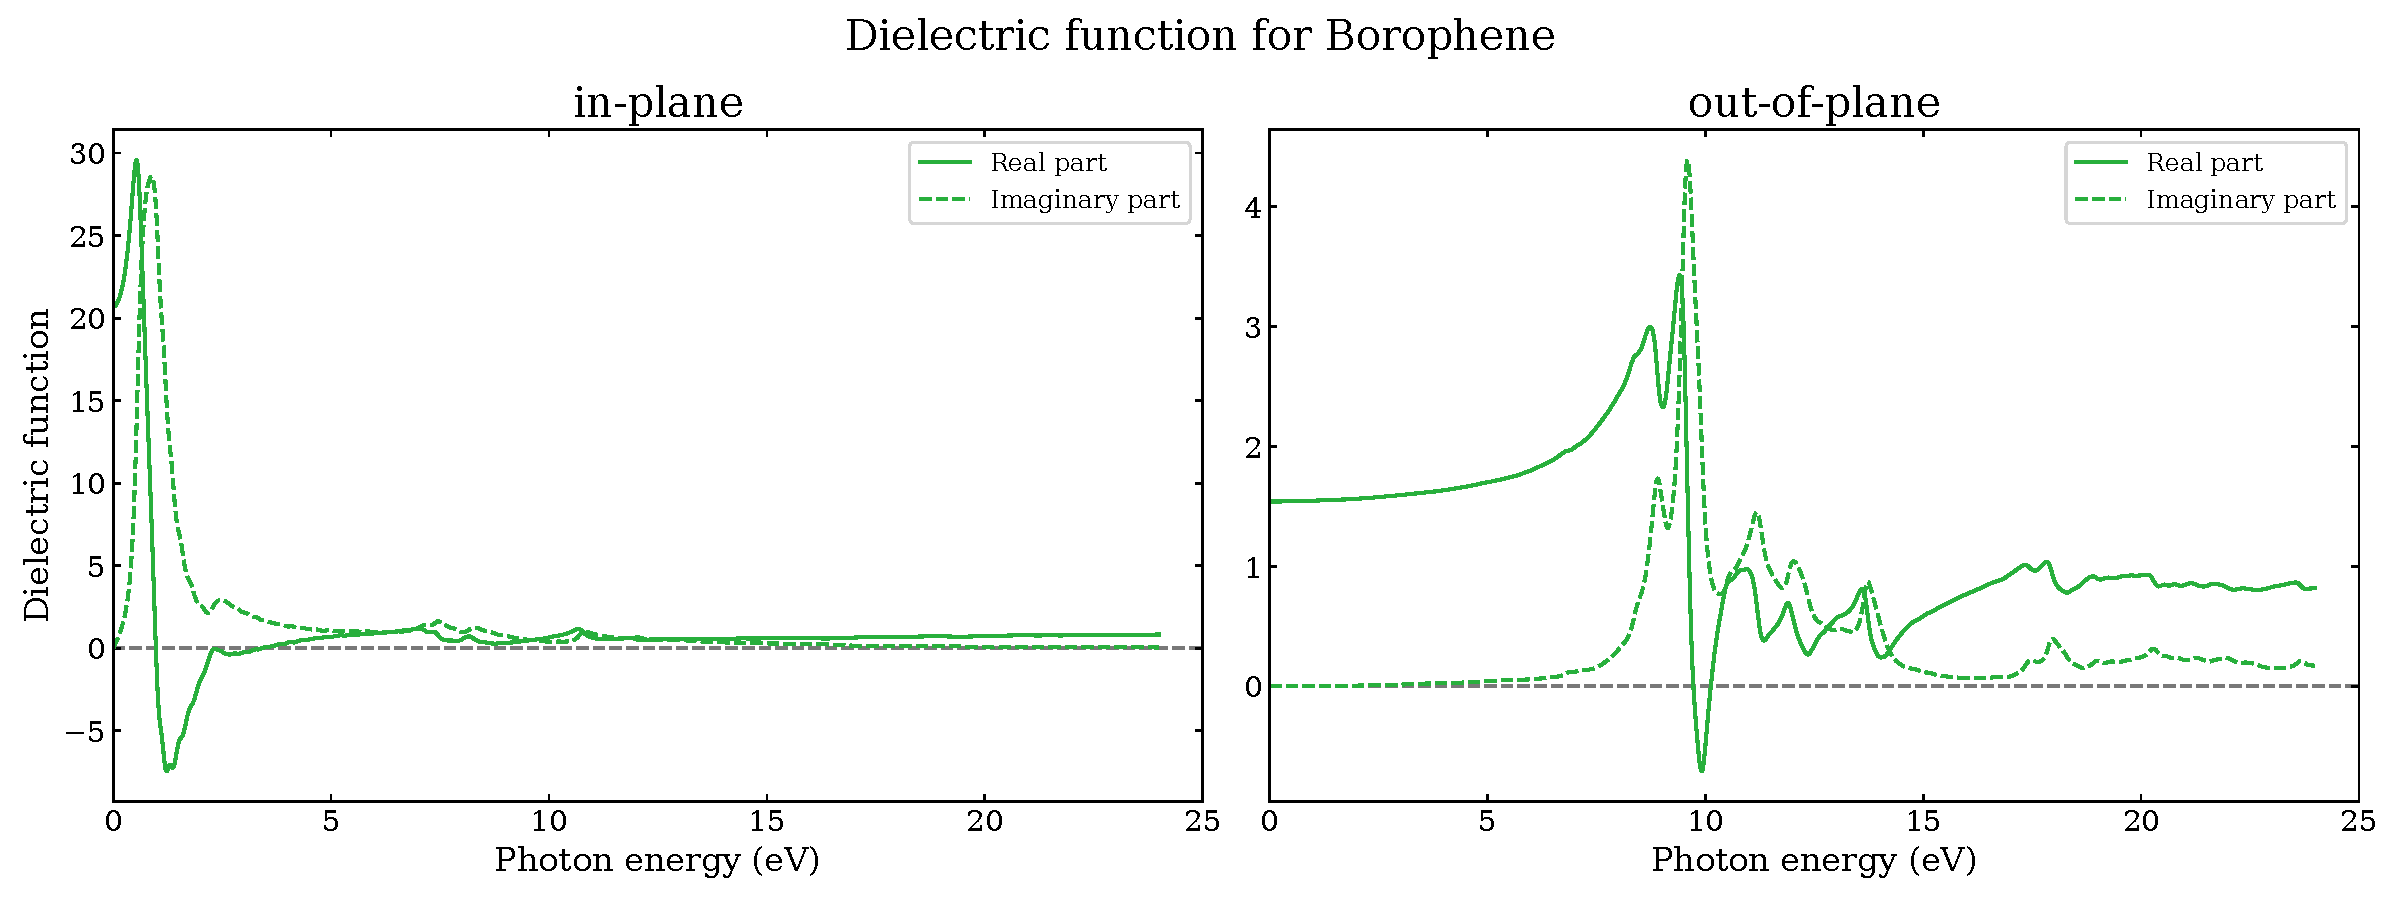
\includegraphics[width=0.80\textwidth]{figures_proj1/S1.13b.pdf}
    \par\nointerlineskip
    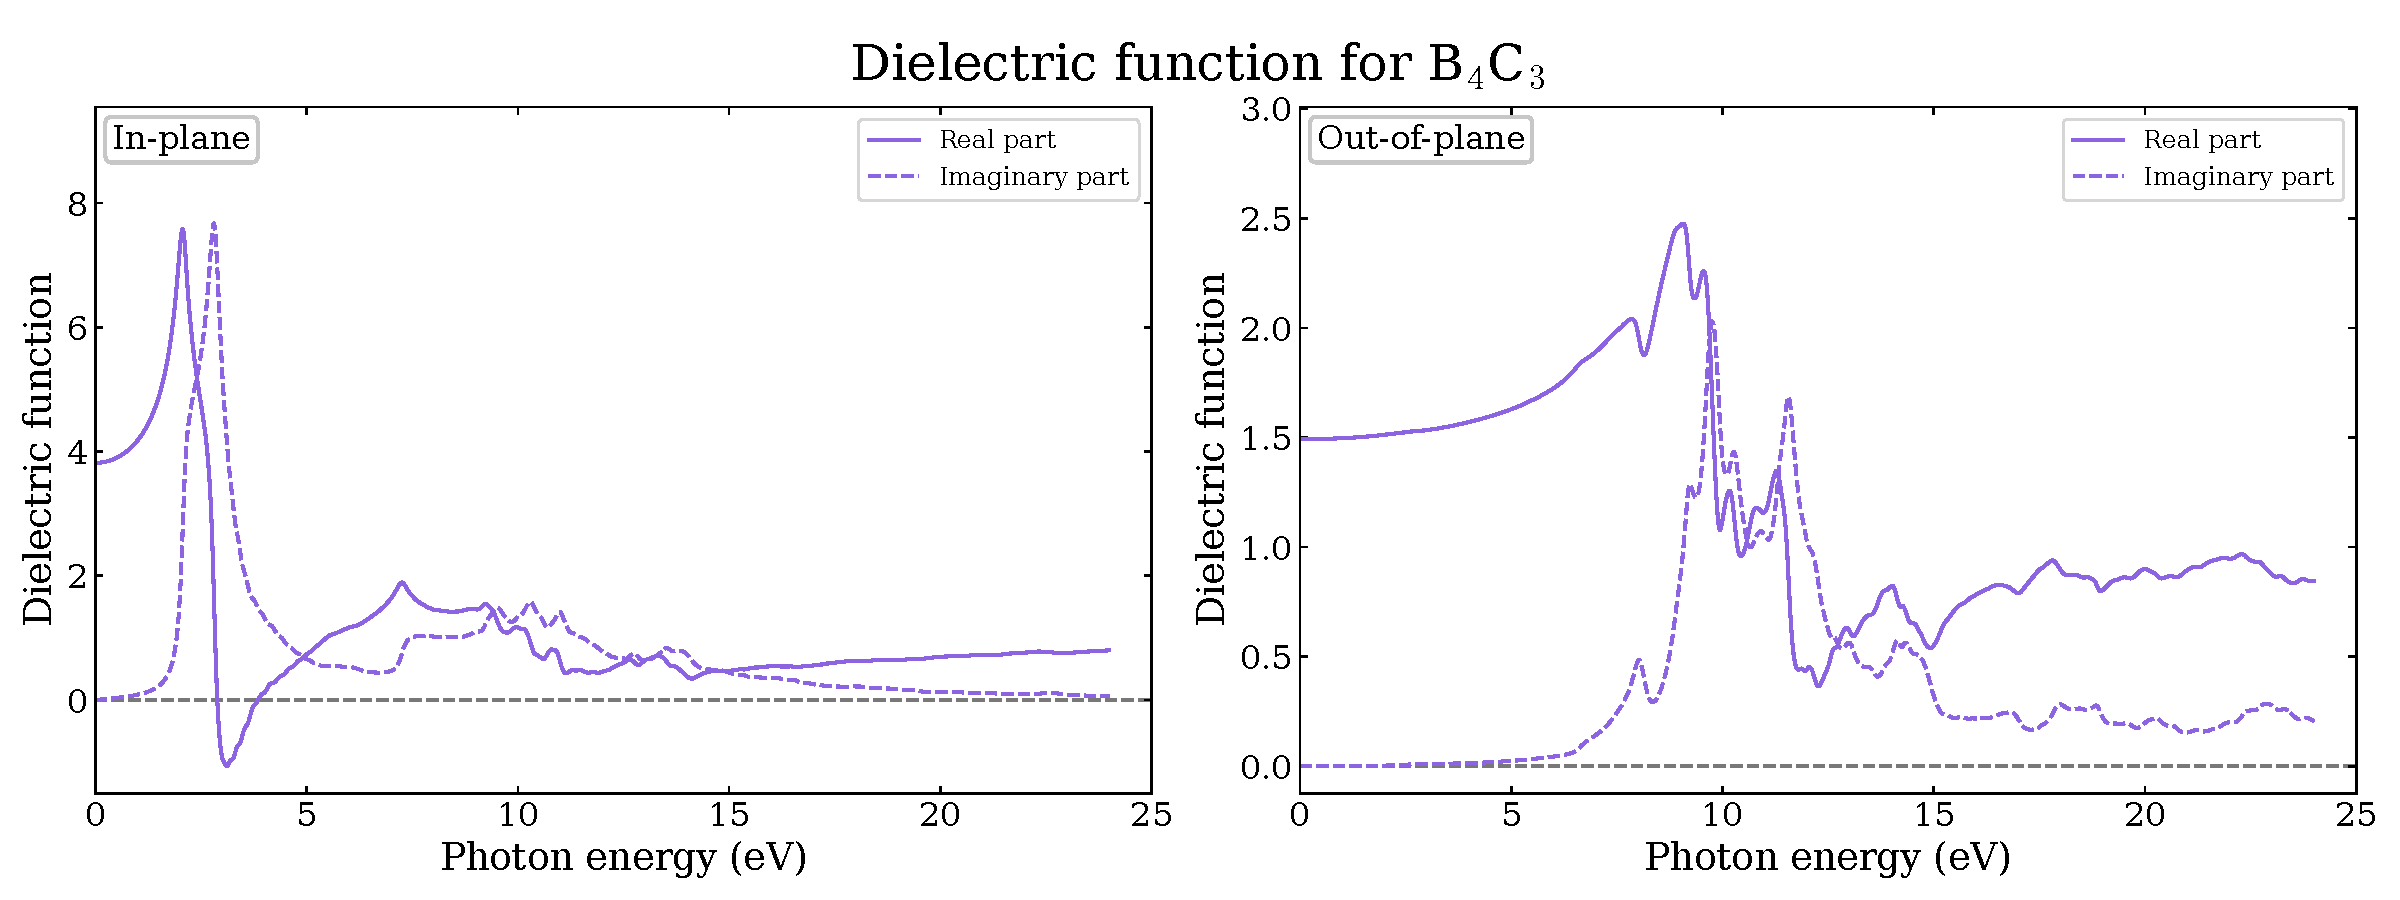
\includegraphics[width=0.80\textwidth]{figures_proj1/S1.13c.pdf}
    \par\nointerlineskip
    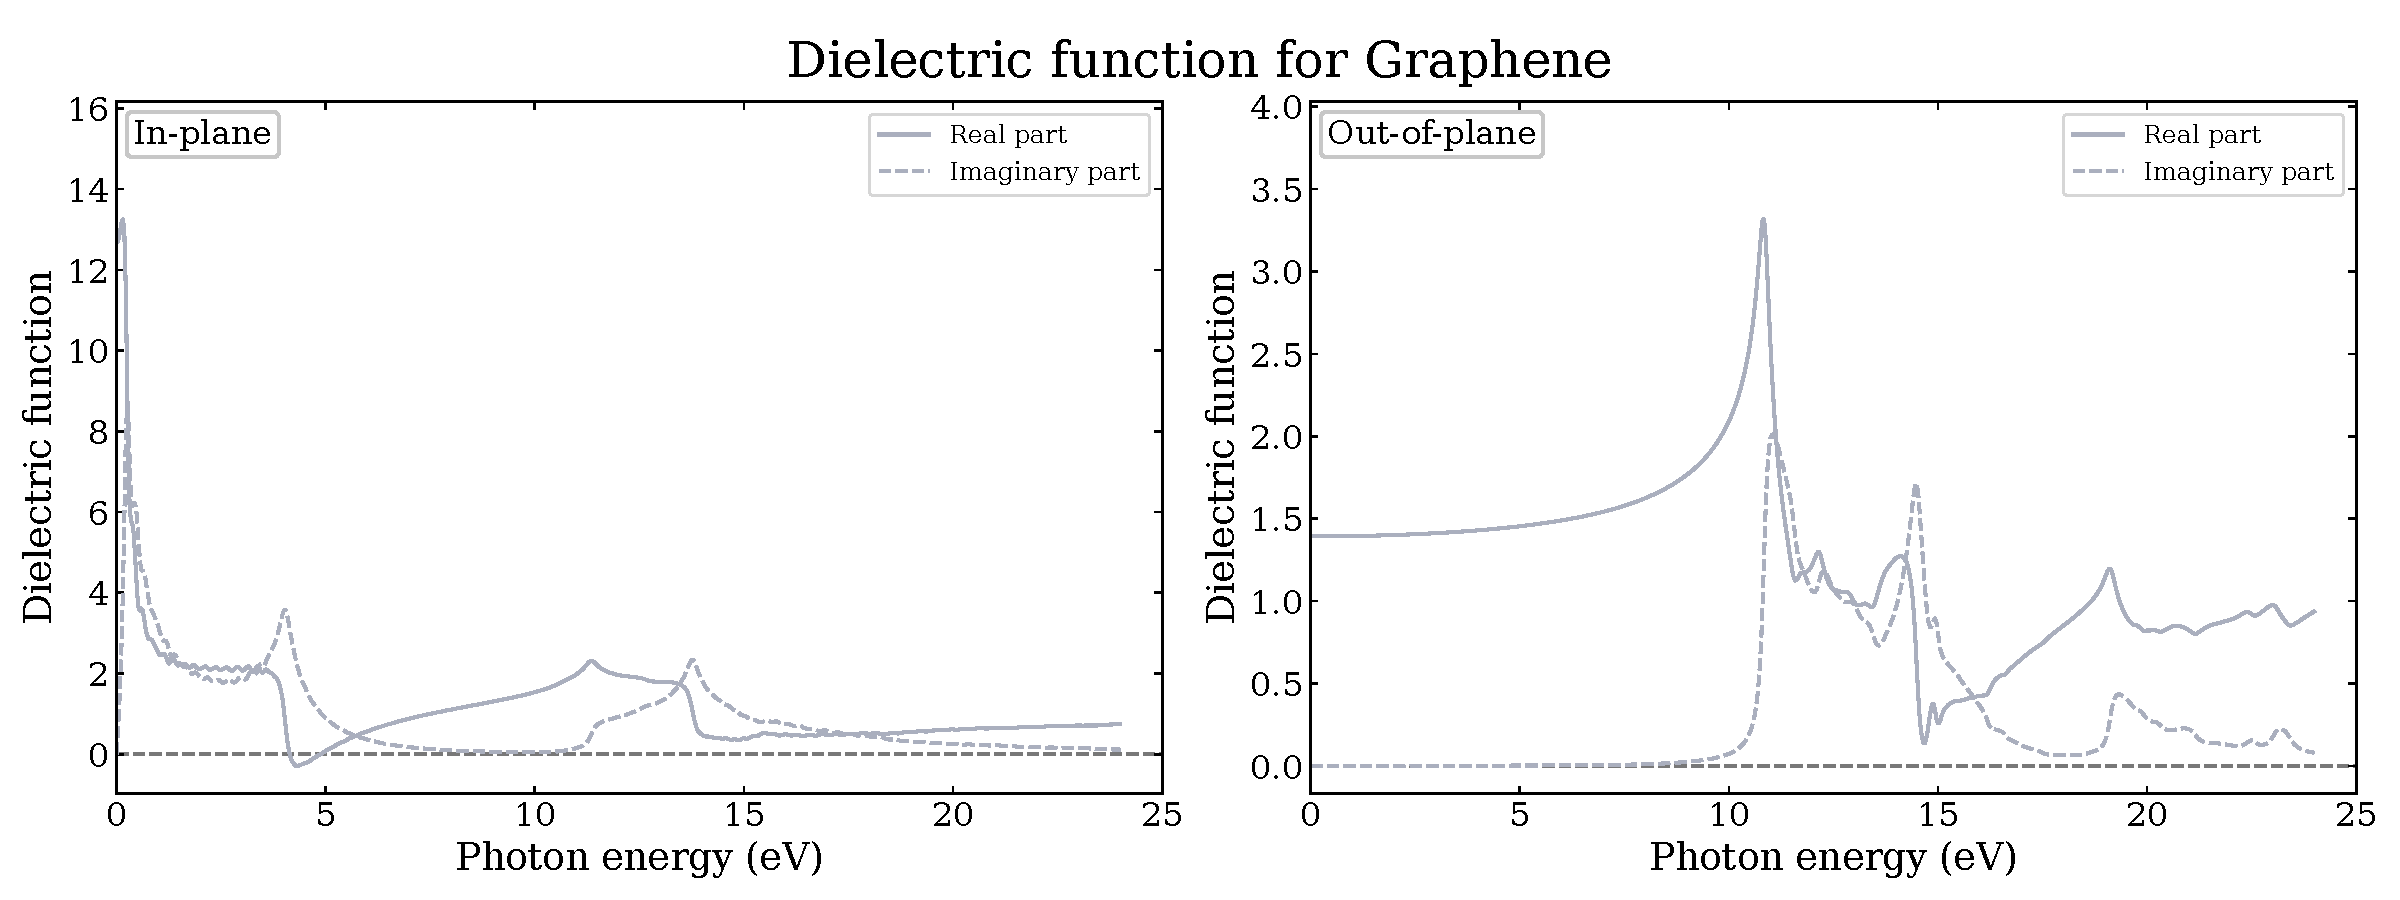
\includegraphics[width=0.80\textwidth]{figures_proj1/S1.13d.pdf}
\caption{Real and imaginary parts of the dielectric function
for the four monolayers as calculated using the PBE functional with a
$129\times 129\times 1$
k-point mesh for graphene,
and a $65\times 65\times 1$
k-point mesh for the borophene and boron-carbide monolayers.
Solid and dashed lines denote the real and imaginary parts, respectively.}
\label{S1.13}
\end{figure}

\begin{figure}[!htbp]
\centering
    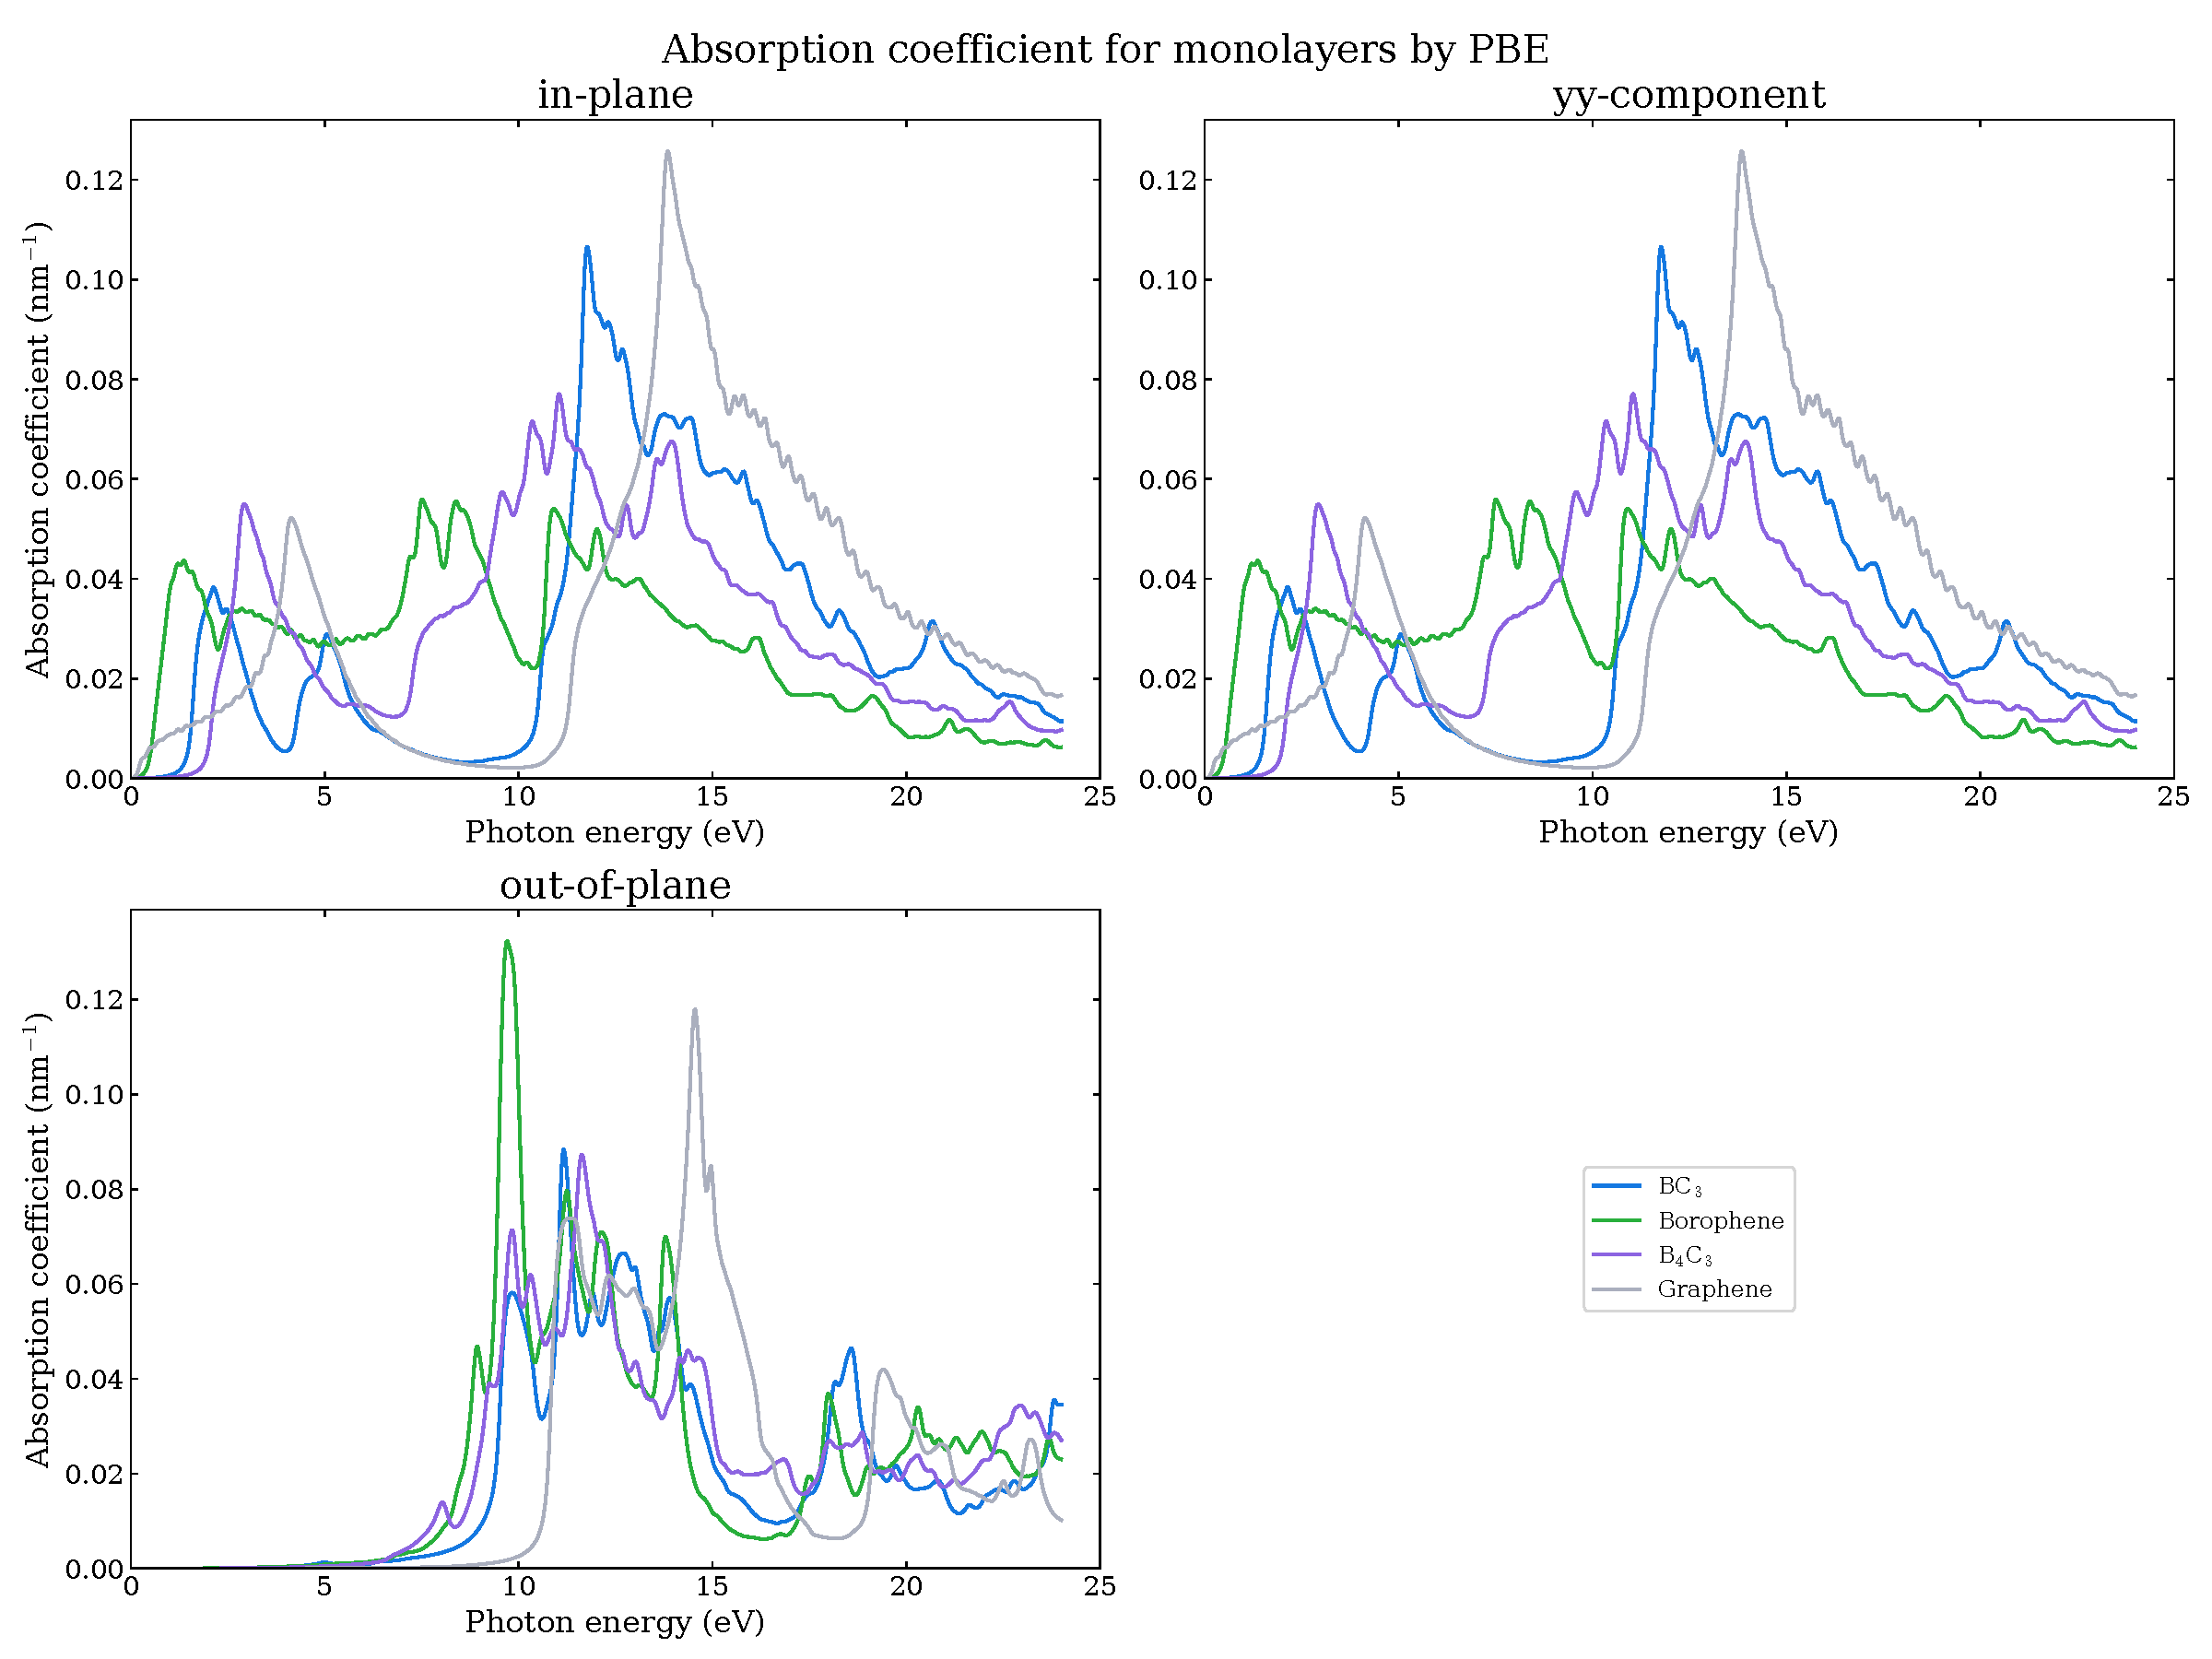
\includegraphics[width=0.80\textwidth]{figures_proj1/S1.14a.pdf}
    \par\nointerlineskip
    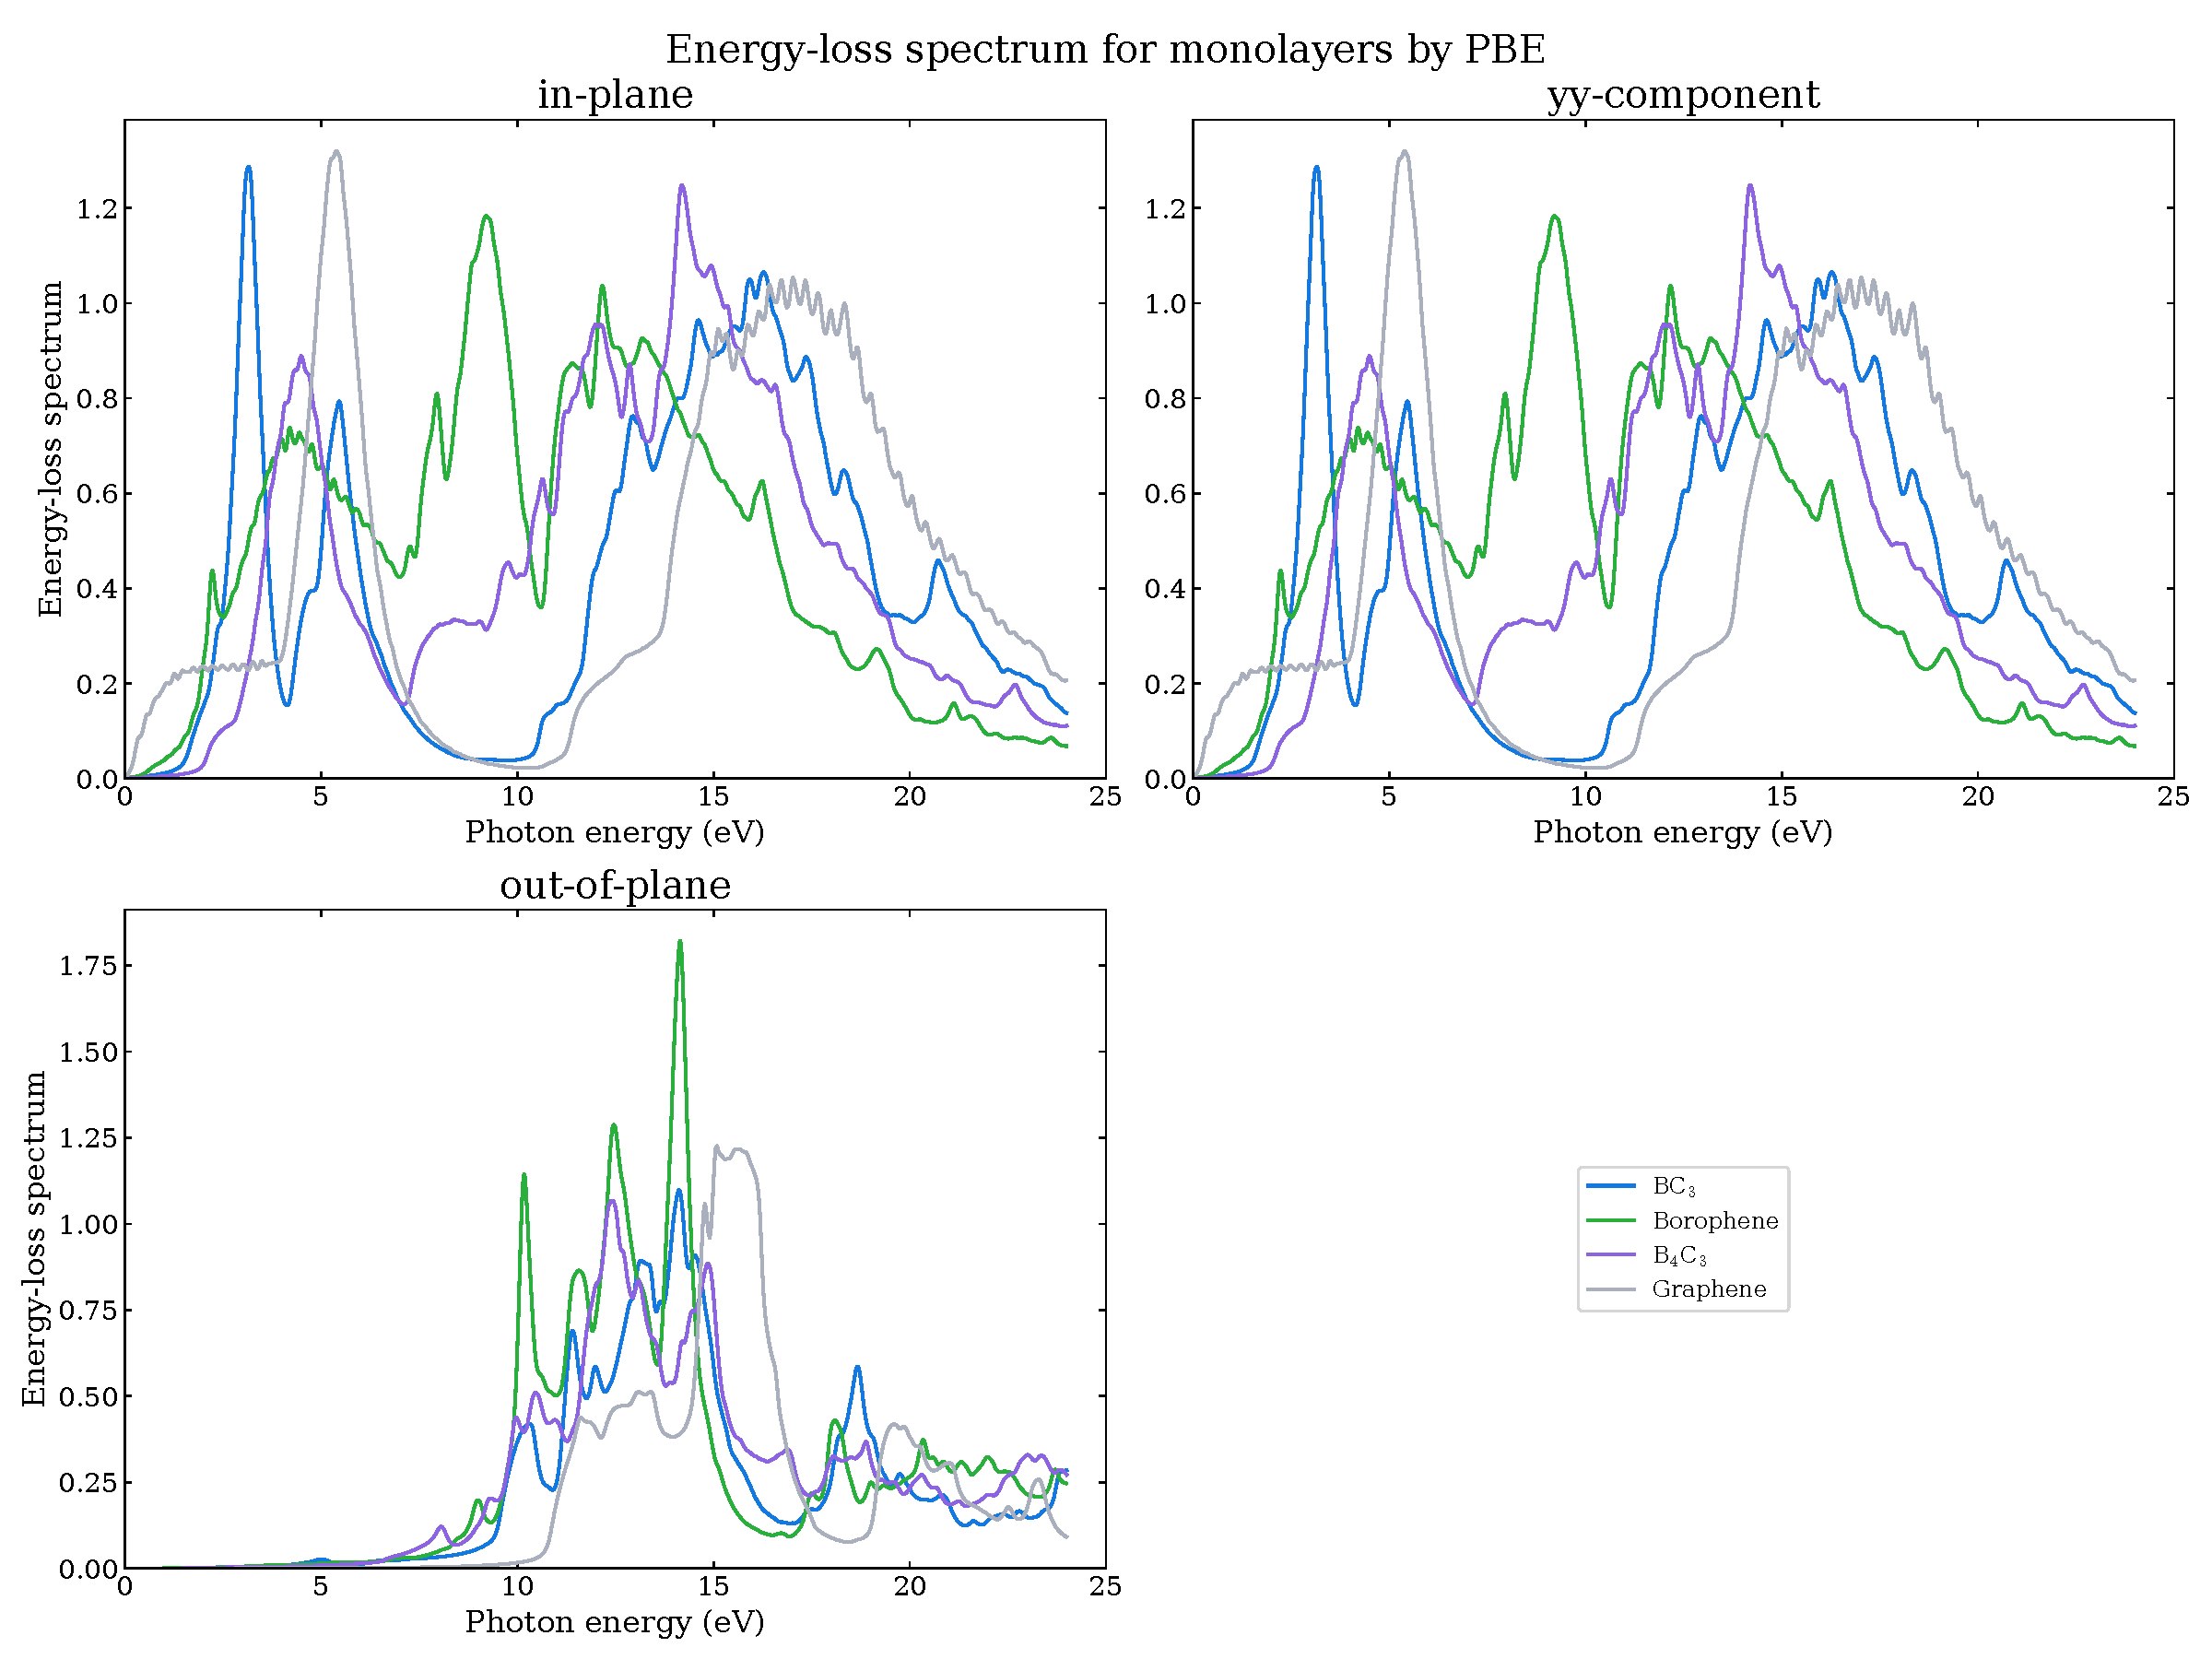
\includegraphics[width=0.80\textwidth]{figures_proj1/S1.14b.pdf}
\caption[Optical properties of the four monolayers calculated using PBE.]{Optical properties of the four monolayers calculated using PBE with the k-point meshes specified in figure~\ref{S1.13}.
Upper: Absorption coefficient in \si{\per\nano\metre}; lower: Dimensionless energy-loss spectrum.}
\label{S1.14}
\end{figure}

\begin{figure}[!htbp]
\ContinuedFloat
\centering
    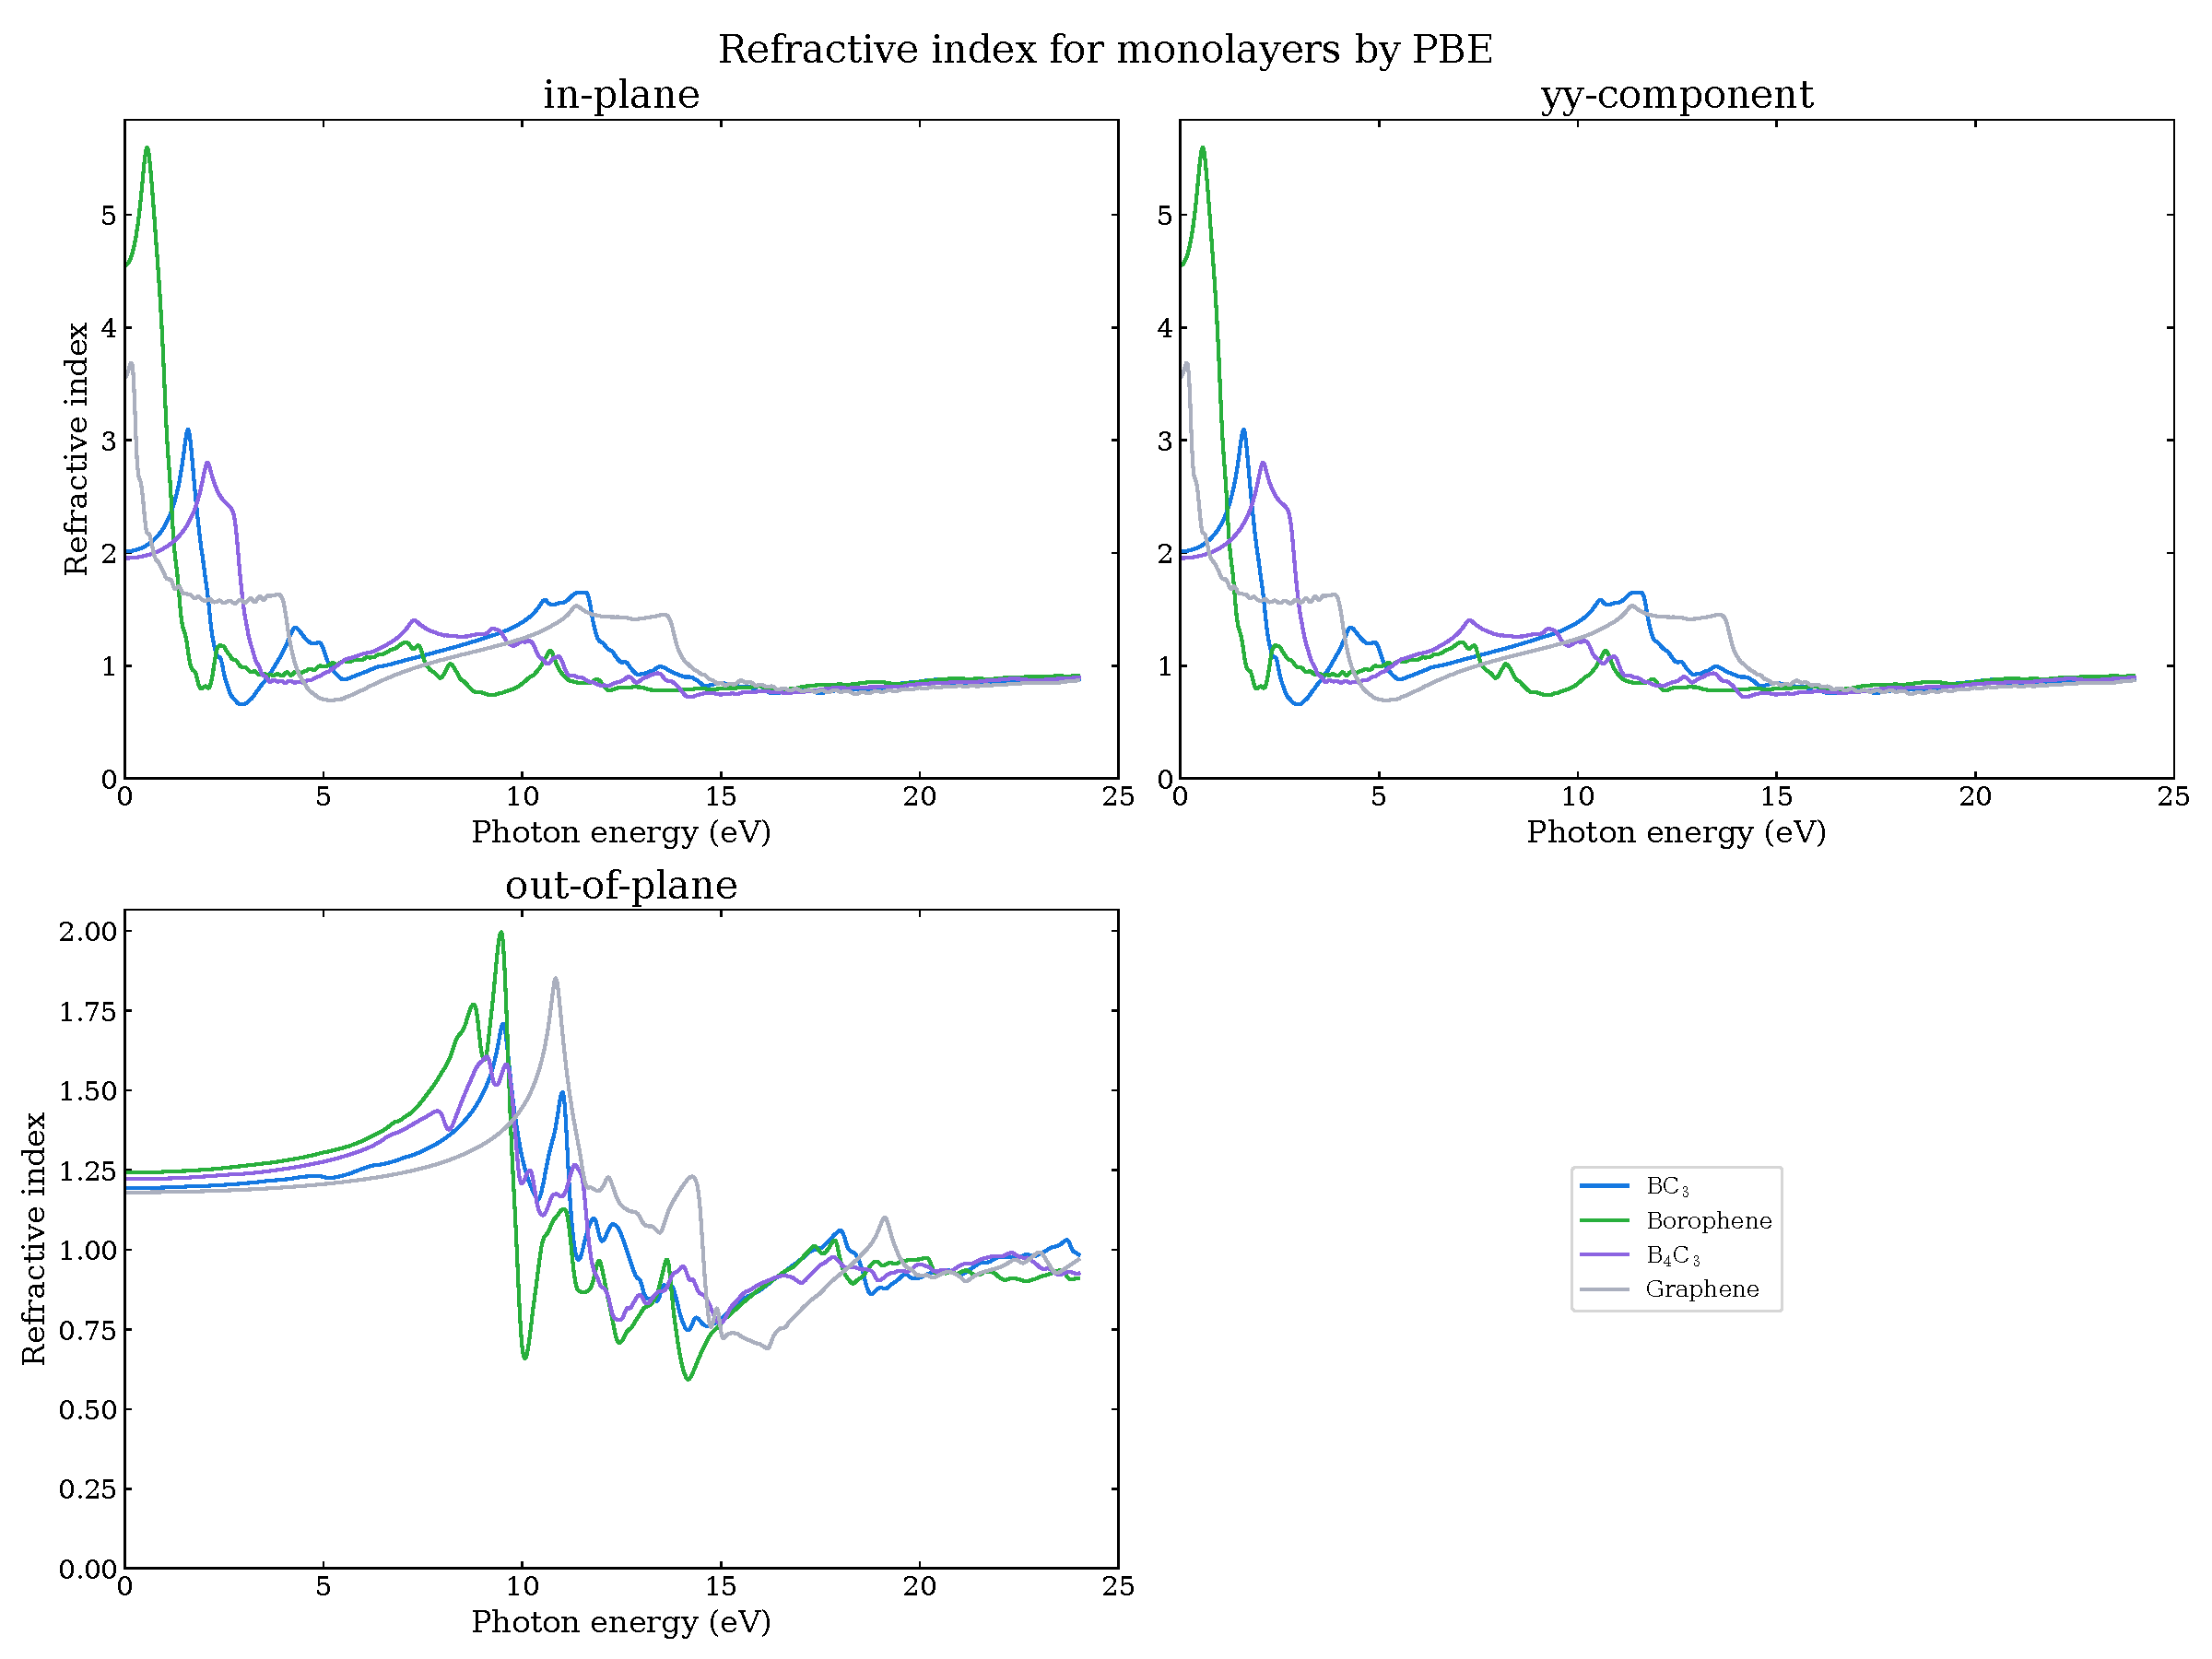
\includegraphics[width=0.80\textwidth]{figures_proj1/S1.14c.pdf}
    \par\nointerlineskip
    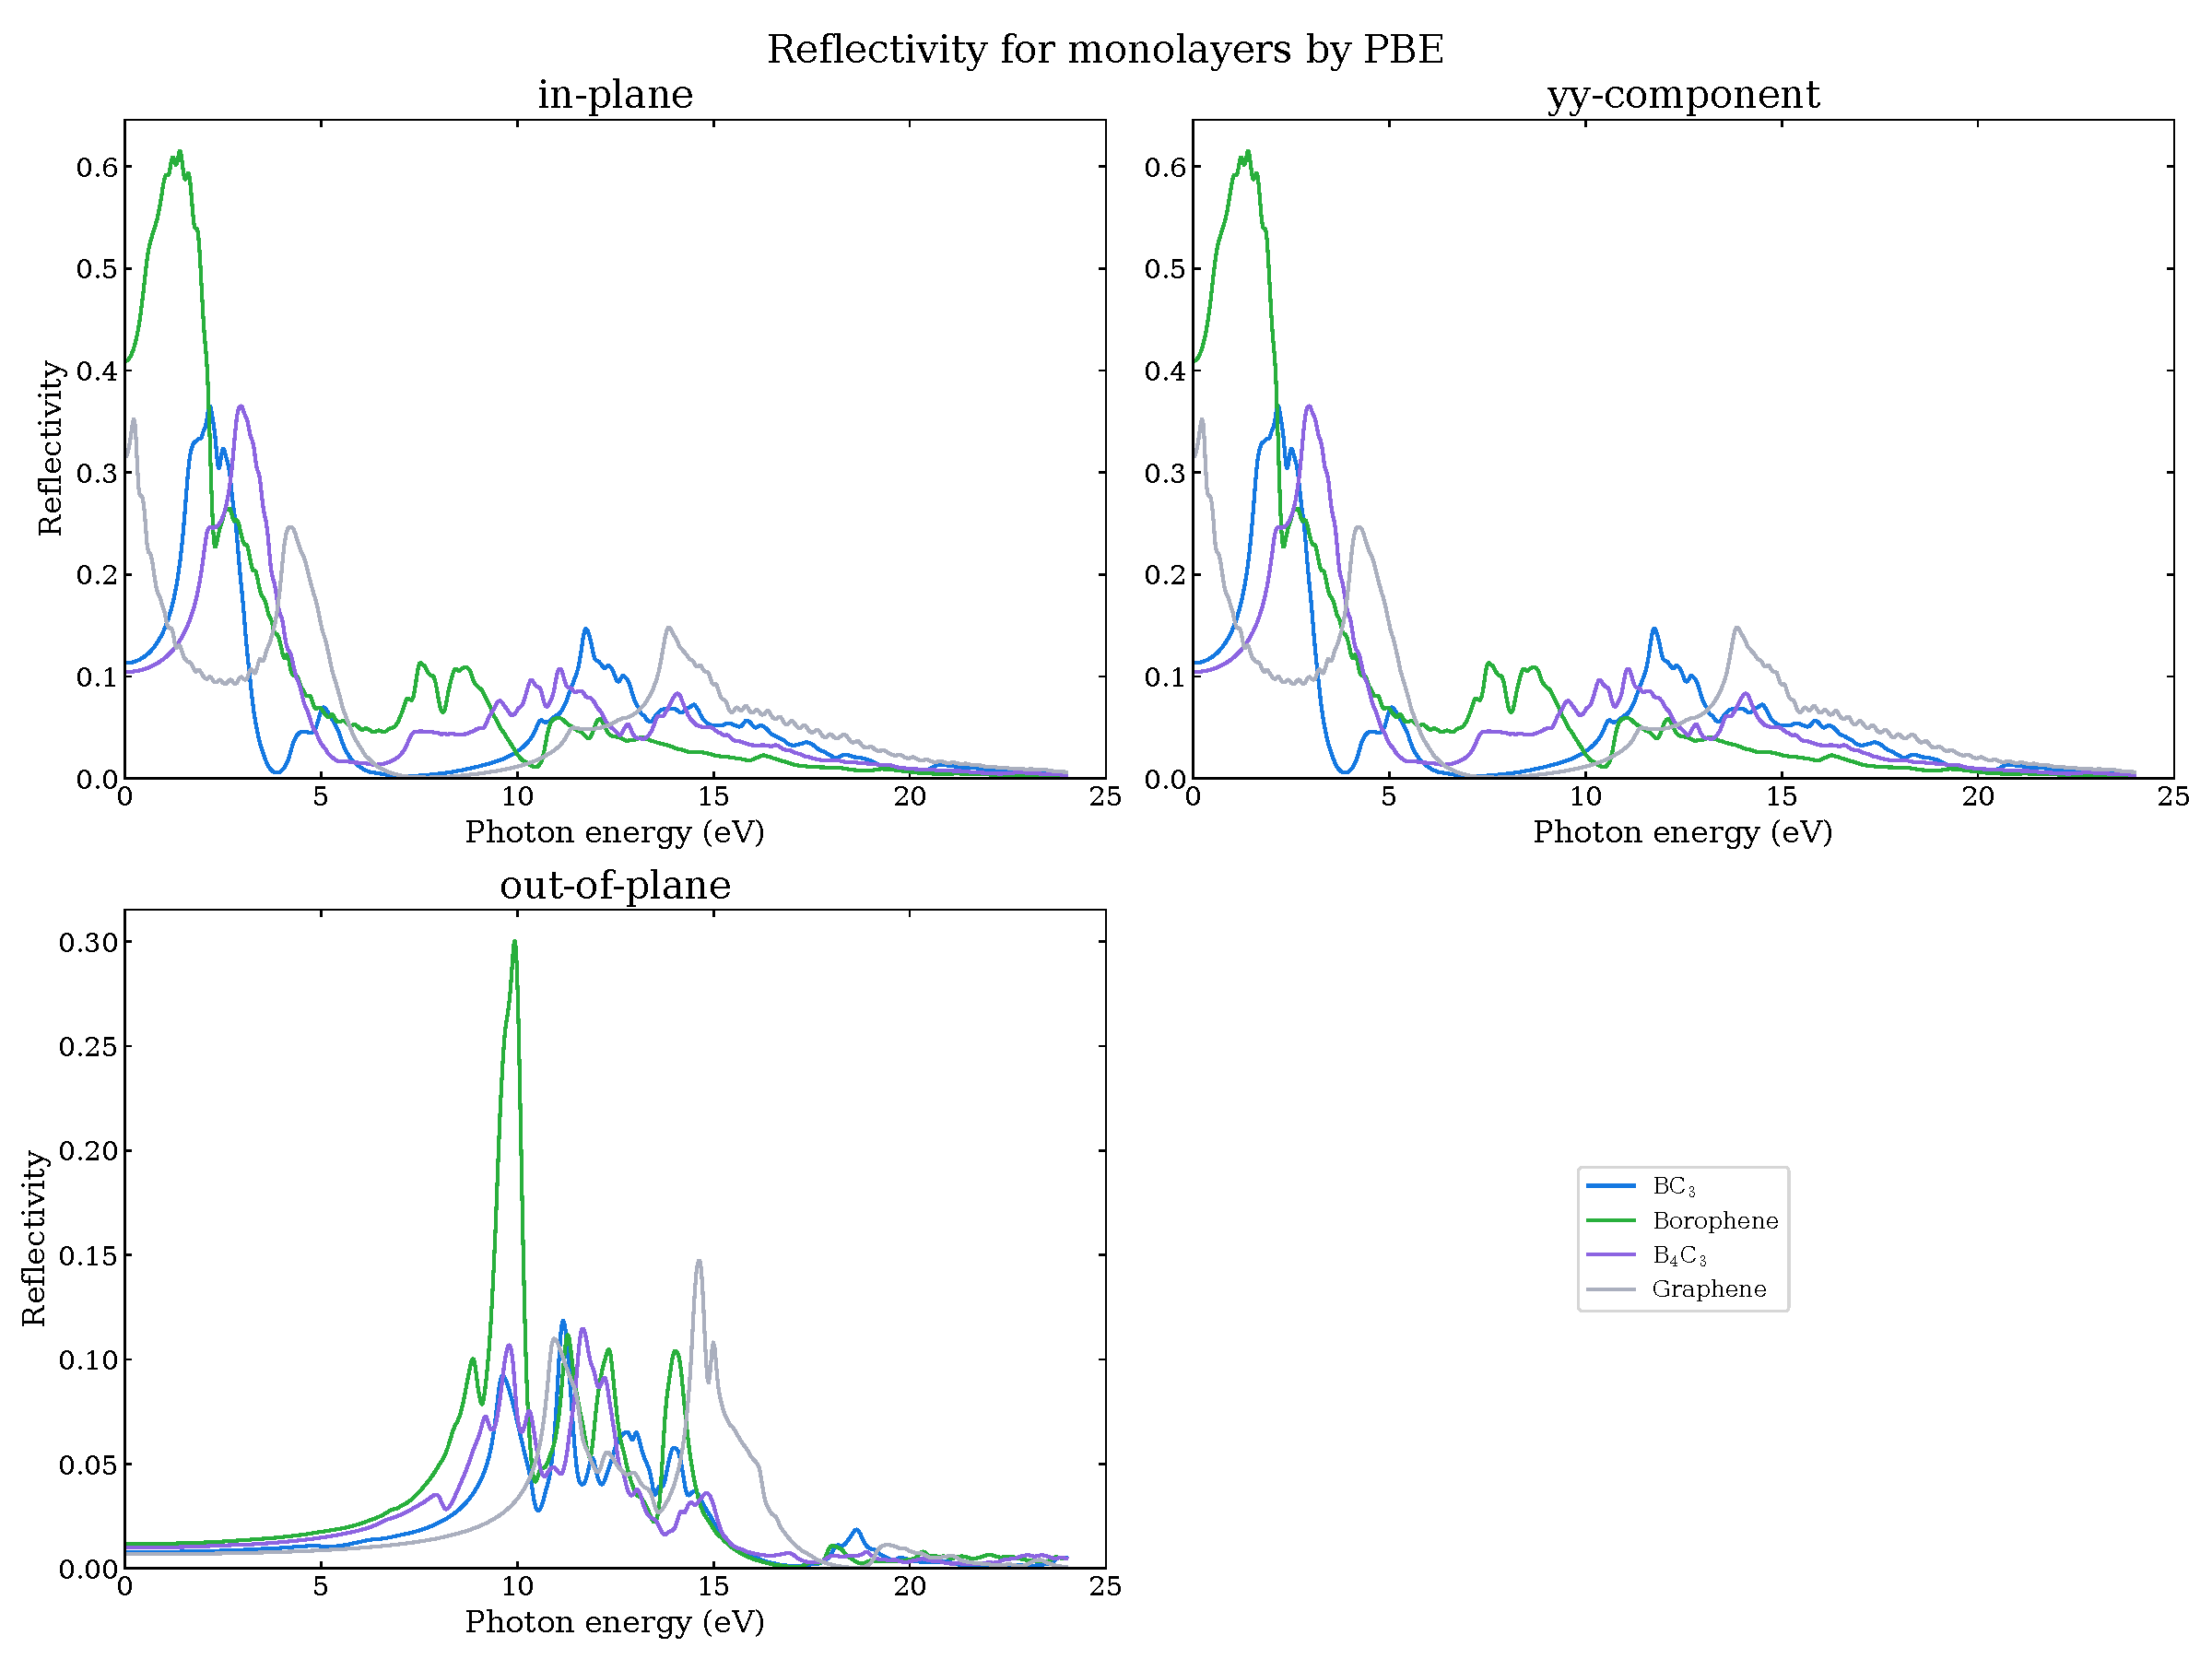
\includegraphics[width=0.80\textwidth]{figures_proj1/S1.14d_correct.pdf}
\caption[]{Optical properties of the four monolayers calculated using PBE (continued).
Upper: Refractive index; lower: Reflectivity.}
\end{figure}

\begin{figure}[!htbp]
\ContinuedFloat
\centering
    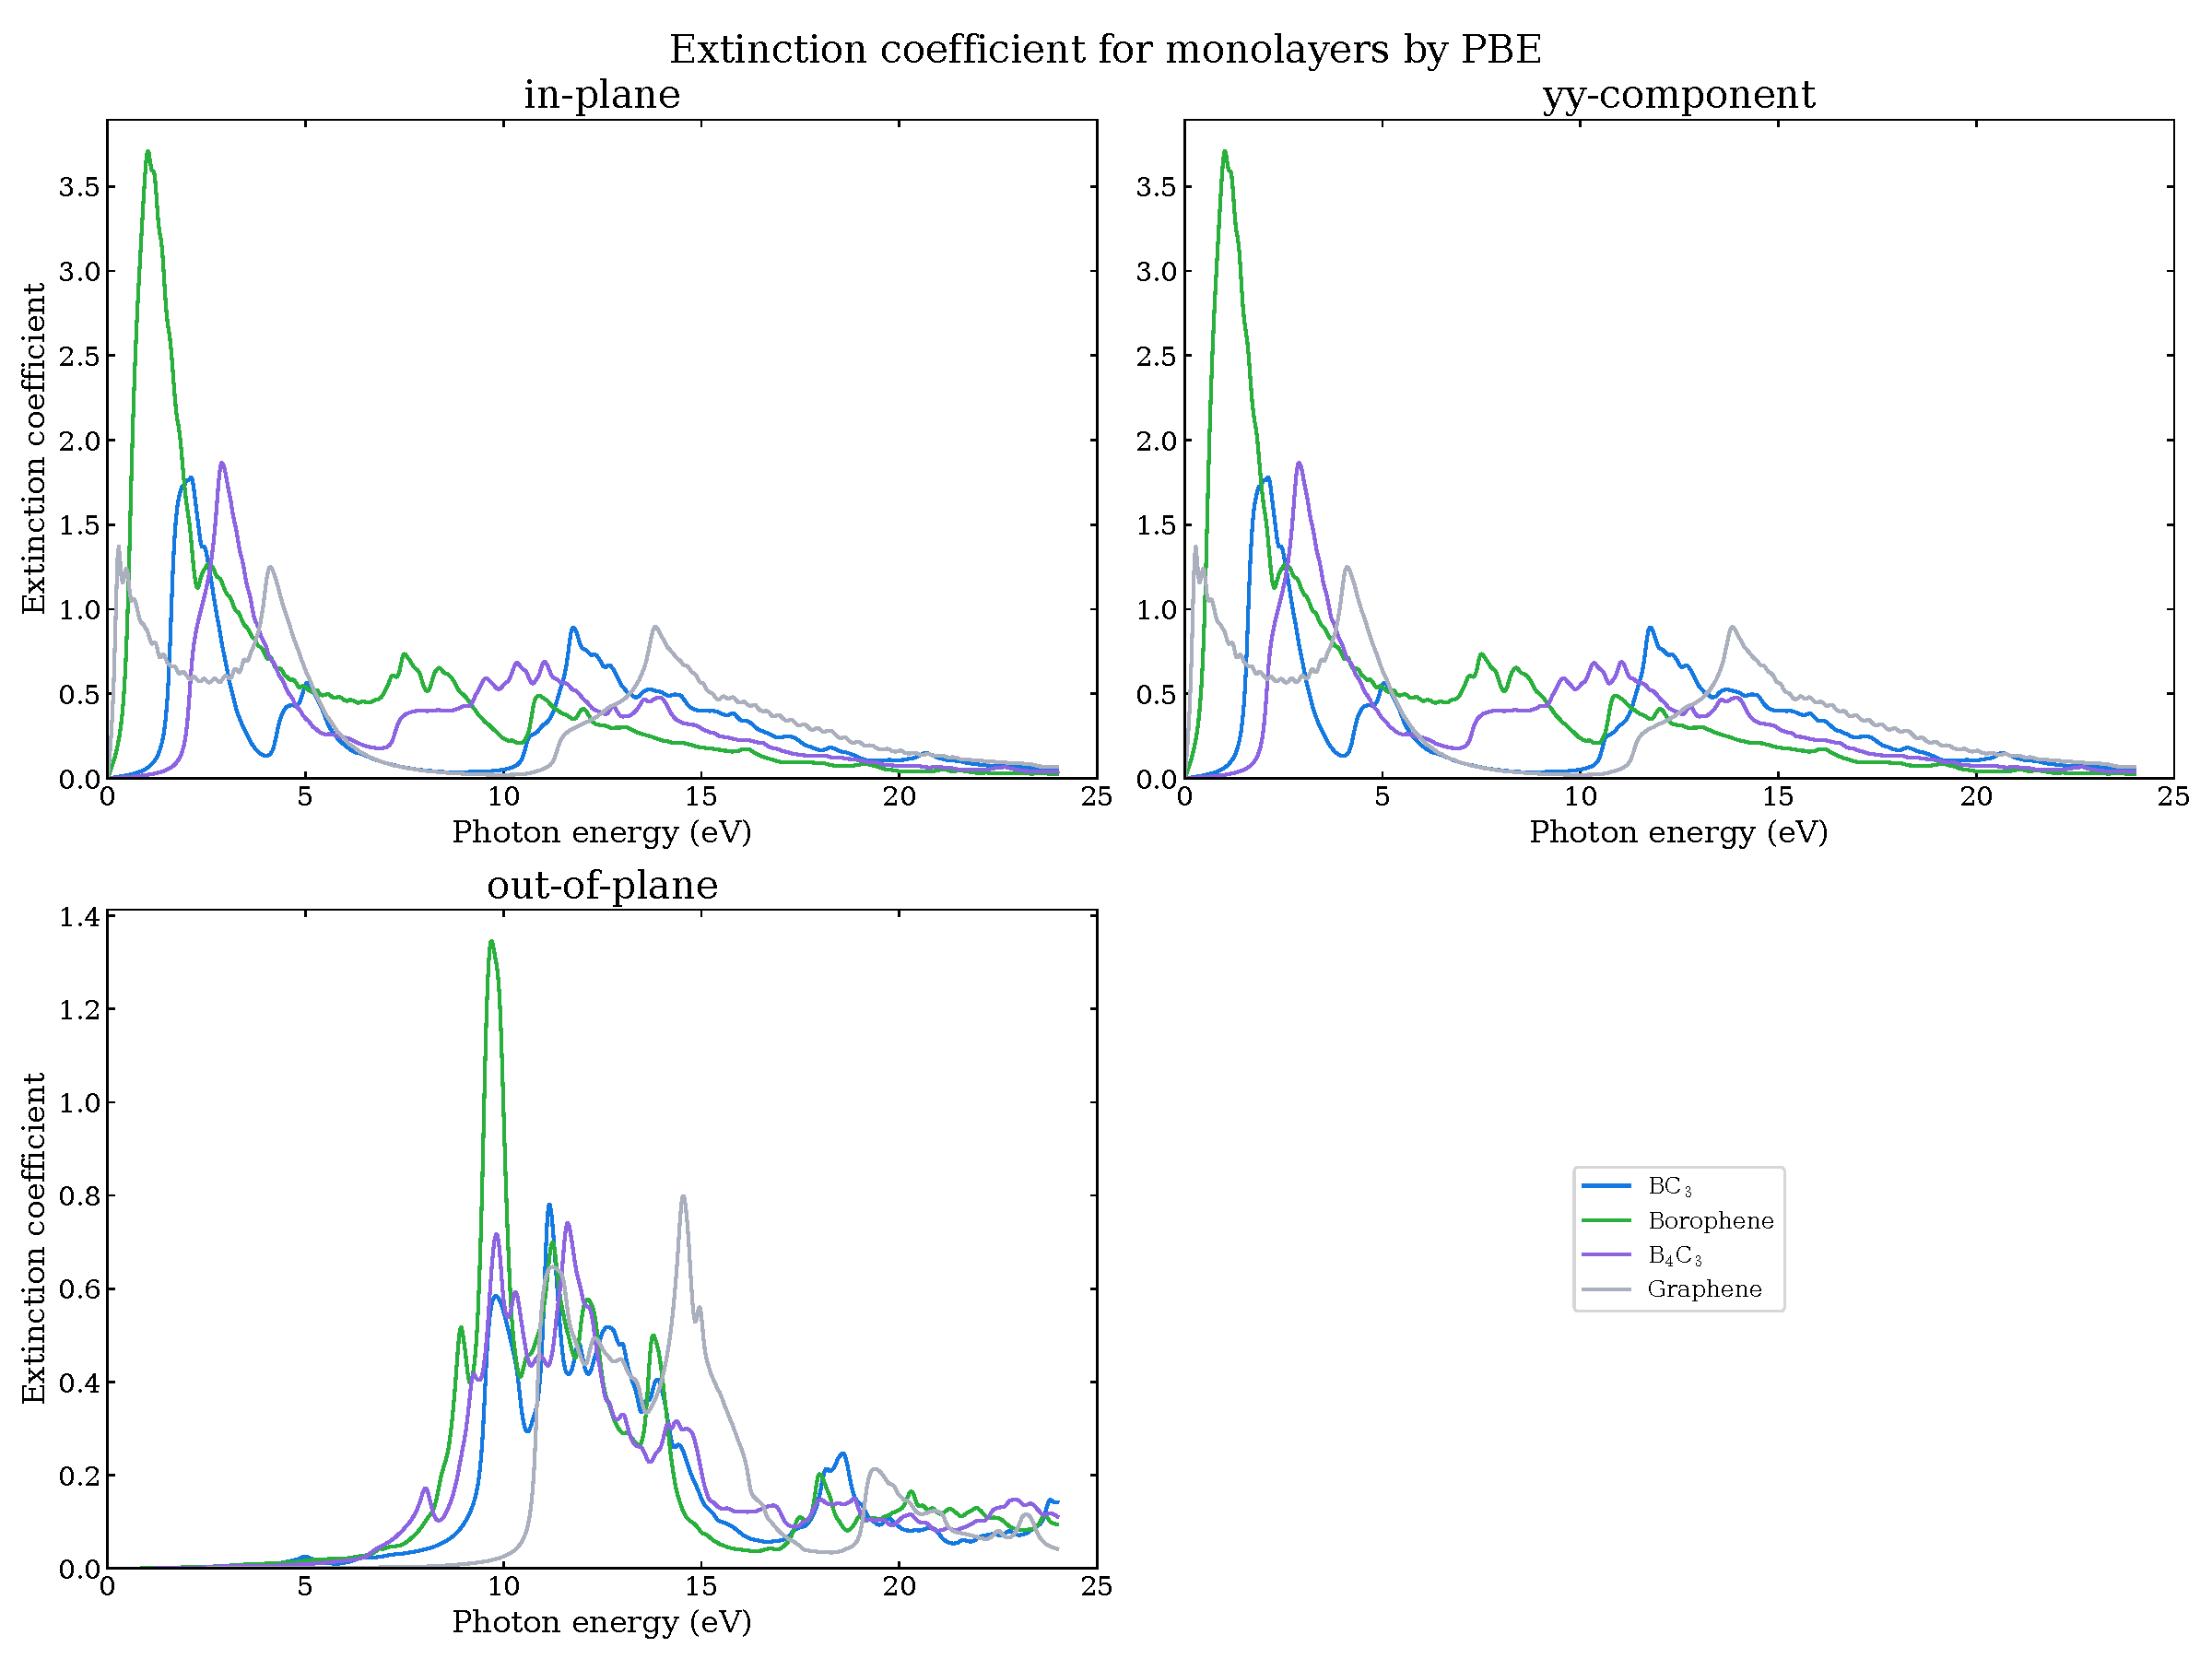
\includegraphics[width=0.80\textwidth]{figures_proj1/S1.14e_correct.pdf}
\caption[]{Optical properties of the four monolayers calculated using PBE (continued): Extinction coefficient.}
\end{figure}

\begin{figure}[!htbp]
\centering
    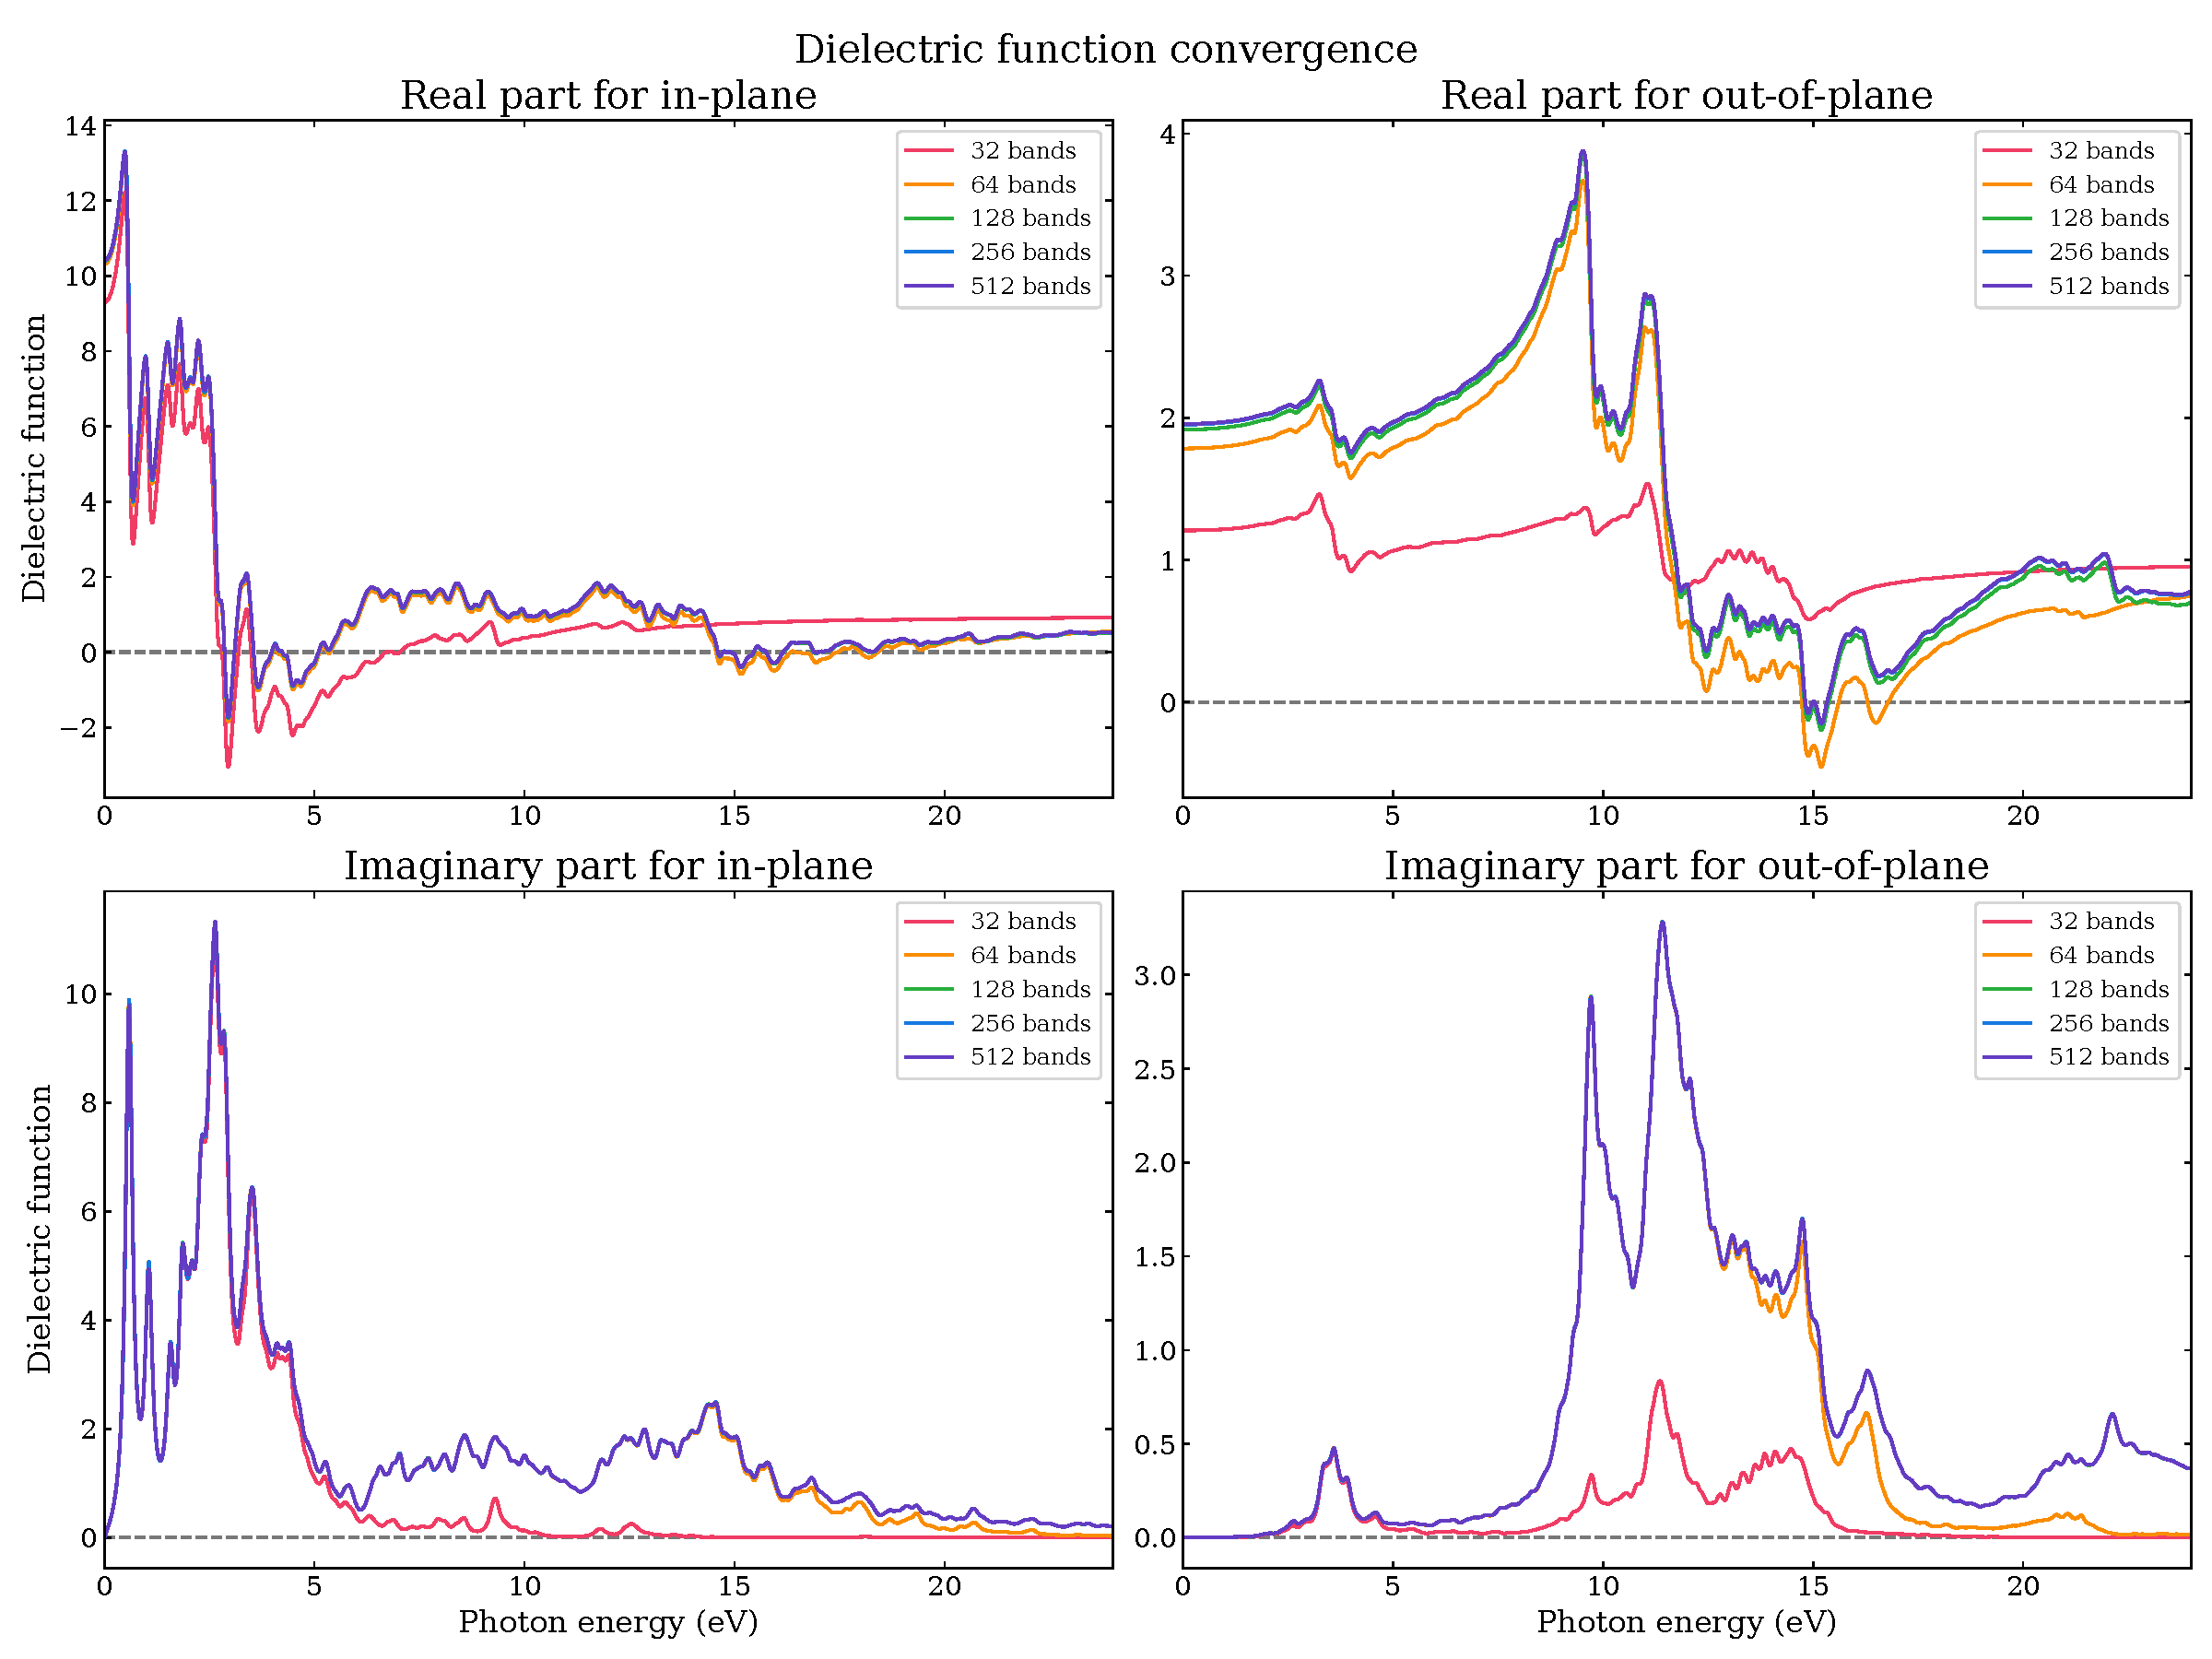
\includegraphics[width=0.80\textwidth]{figures_proj1/S1.15.pdf}
\caption{Convergence test of the dielectric function of Graphene-\ce{B4C3} with respect to the total number of bands, including unoccupied states, calculated using PBE.}
\label{S1.15}
\end{figure}

Figure~\ref{S1.16} also shows the effect of the energy convergence criterion \texttt{EDIFF} on the calculated dielectric function, together with the effects of different k-point meshes and the comparison between HSE06 and PBE.

\begin{figure}[!htbp]
\centering
    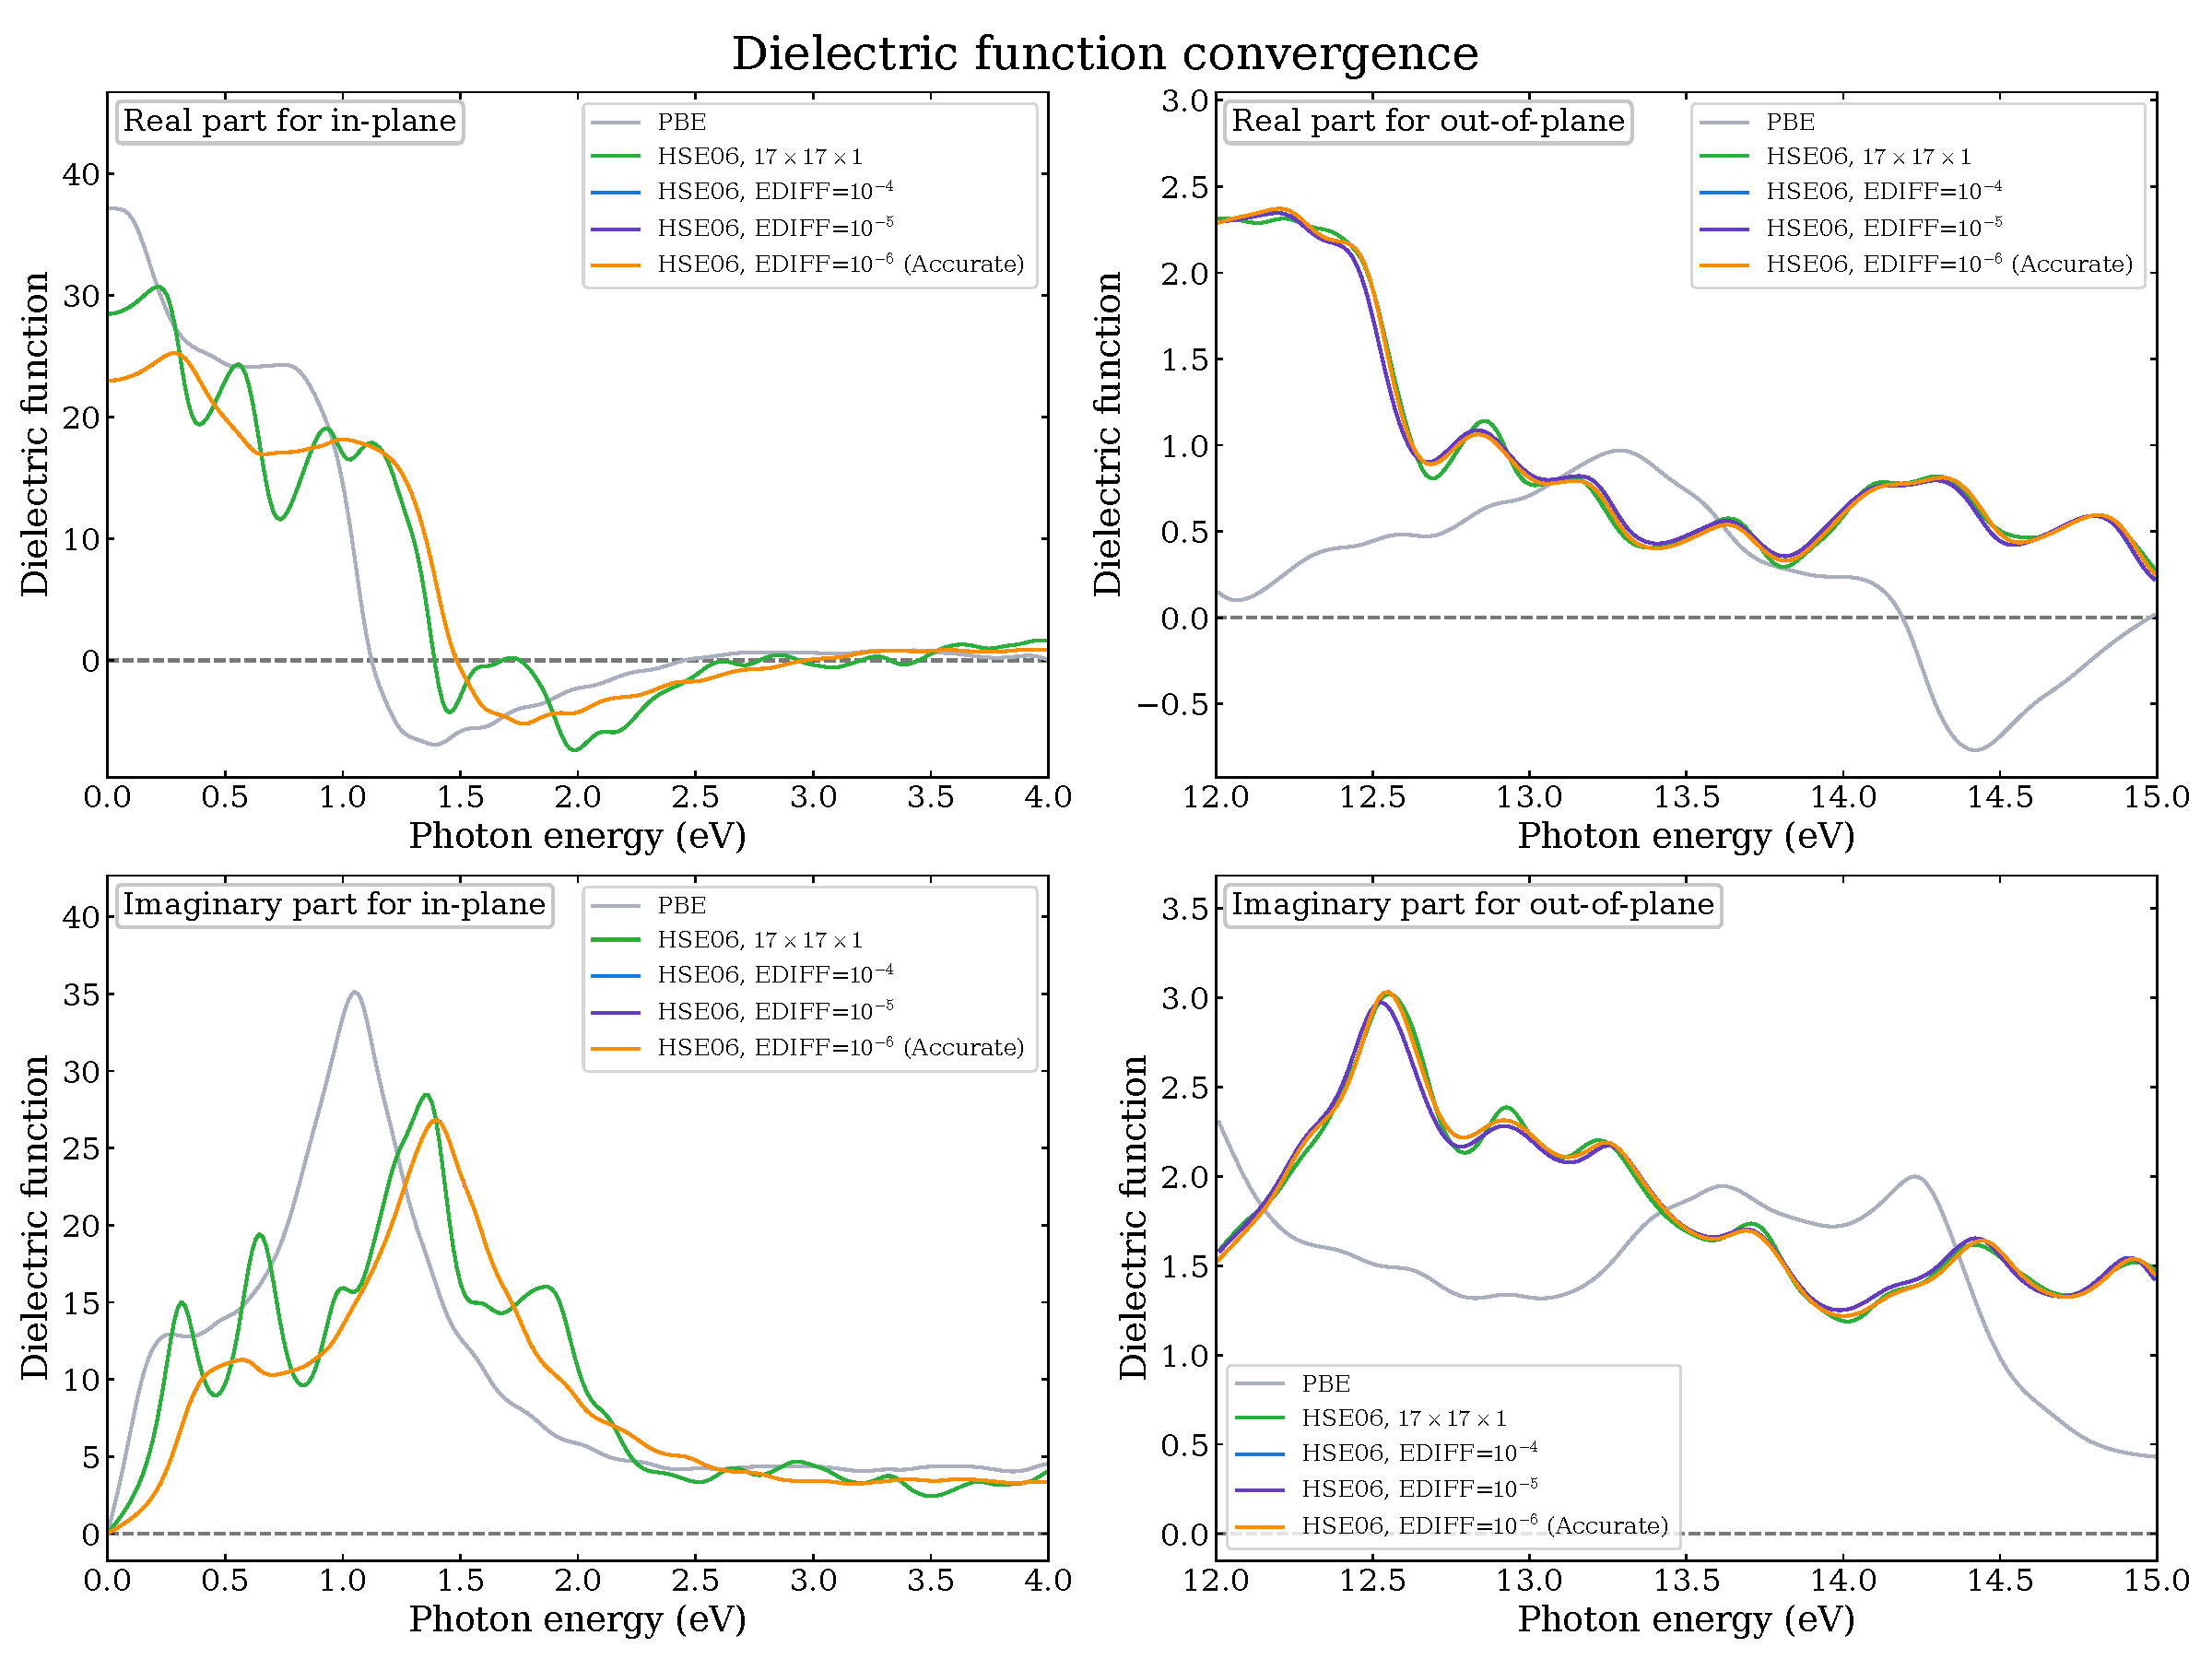
\includegraphics[width=0.80\textwidth]{figures_proj1/S1.16_alt.pdf}
\caption[Dielectric-function convergence tests for the Graphene-Borophene bilayer.]{Dielectric function of the Graphene-Borophene bilayer comparing PBE and HSE06 results, HSE06 k-point meshes of $17 \times 17 \times 1$ and $65 \times 65 \times 1$, and HSE06 energy convergence criteria \texttt{EDIFF} = $10^{-4}$, $10^{-5}$, and $10^{-6}$.
The $10^{-4}$ and $10^{-5}$ calculations use \texttt{PREC=Normal}, while the $10^{-6}$ calculation uses \texttt{PREC=Accurate}.}
\label{S1.16}
\end{figure}

Figures~\ref{S1.17}--\ref{S1.19} show the full dielectric-function tensor components of the three bilayer systems,
as calculated using both the PBE and HSE06 functionals.
The diagonal components describe the dominant in-plane and out-of-plane optical responses,
whereas the off-diagonal components describe the coupling between different Cartesian directions.
The displayed off-diagonal components are negligible for Graphene-Borophene,
but remain finite for Graphene-\ce{BC3} and Graphene-\ce{B4C3}.
Their opposite-sign pairs require the tensor-symmetry check discussed in the main text;
they are retained here to identify the original calculated spectra and are not evidence of optical activity.

In addition, figures~\ref{S1.20}--\ref{S1.24} compare the optical properties derived from the diagonal HSE06 dielectric components for the three bilayer heterostructures.
These properties include the absorption coefficient, energy-loss spectrum, refractive index, reflectivity, and extinction coefficient.
The $xx$ and $yy$ components correspond to electric-field polarizations within the layers,
whereas $zz$ corresponds to polarization perpendicular to the layers.
The scalar relations introduced in chapter~\ref{cha:fundamentals_b} do not define separate optical observables for the off-diagonal elements.
The diagonal results below use an effective principal-axis description;
for the tensors with finite off-diagonal components, this remains conditional on resolving the tensor-symmetry issue.

\begin{figure}[!htbp]
\centering
    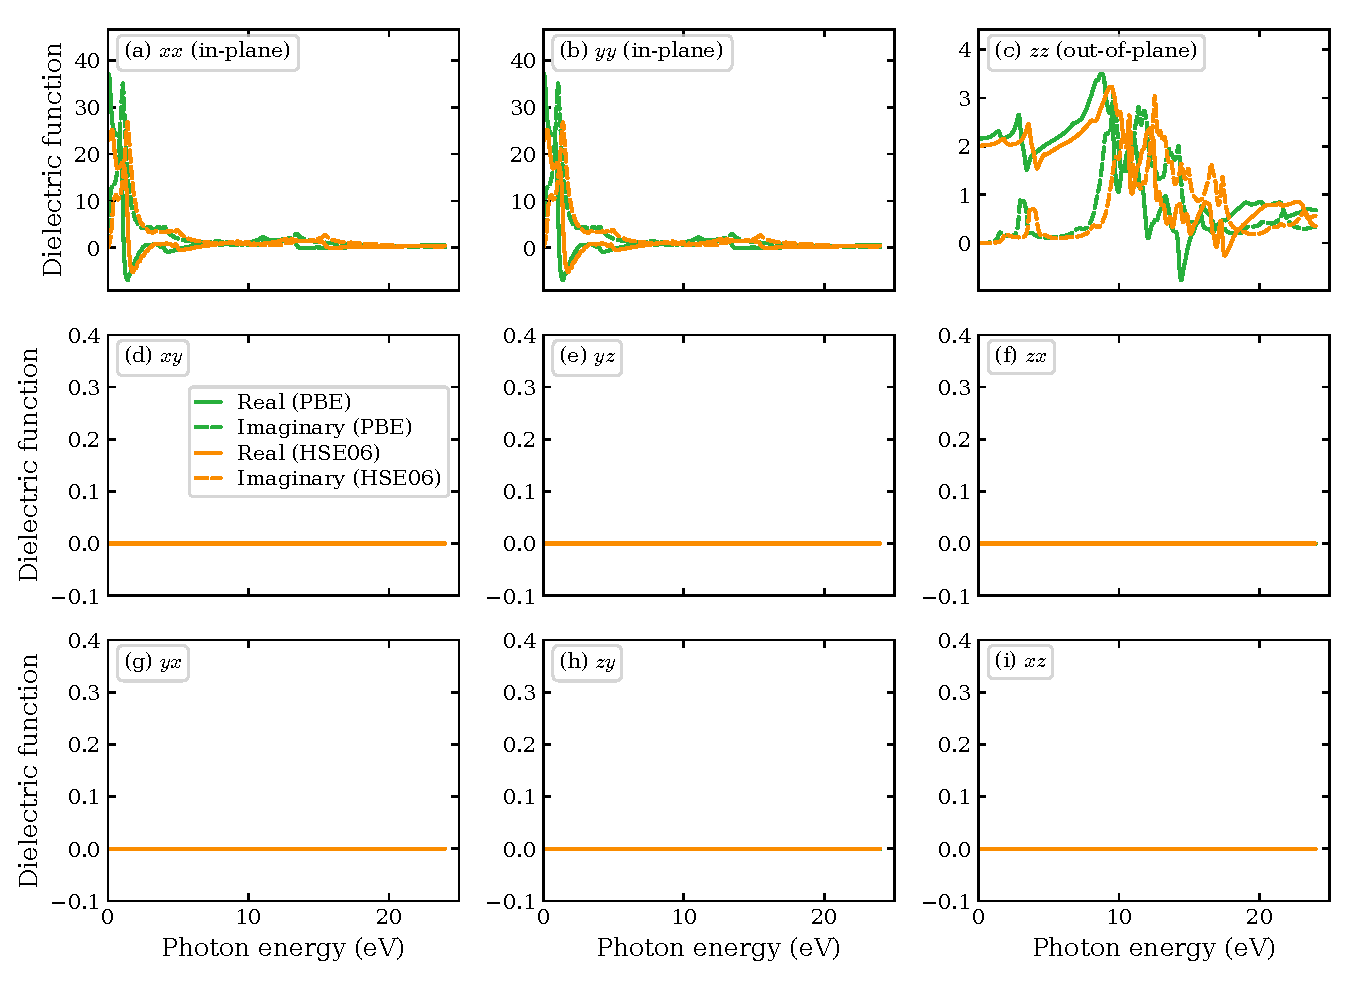
\includegraphics[width=1.00\textwidth]{figures_proj1/S1.17_alt.pdf}
\caption[Dielectric tensor of Graphene-Borophene calculated using PBE and HSE06.]{Dimensionless dielectric tensor components of Graphene-Borophene versus photon energy $\hbar\omega$ in \unit{\electronvolt}.
From left to right, the rows show $xx,yy,zz$; $xy,yz,zx$; and $yx,zy,xz$.
The $xx$ and $yy$ directions lie within the layers, while $zz$ is perpendicular to them.
Green and orange curves denote PBE and HSE06, respectively; solid and dashed lines denote real and imaginary parts.
The off-diagonal components are negligible on the plotted scale.}
\label{S1.17}
\end{figure}

\begin{figure}[!htbp]
\centering
    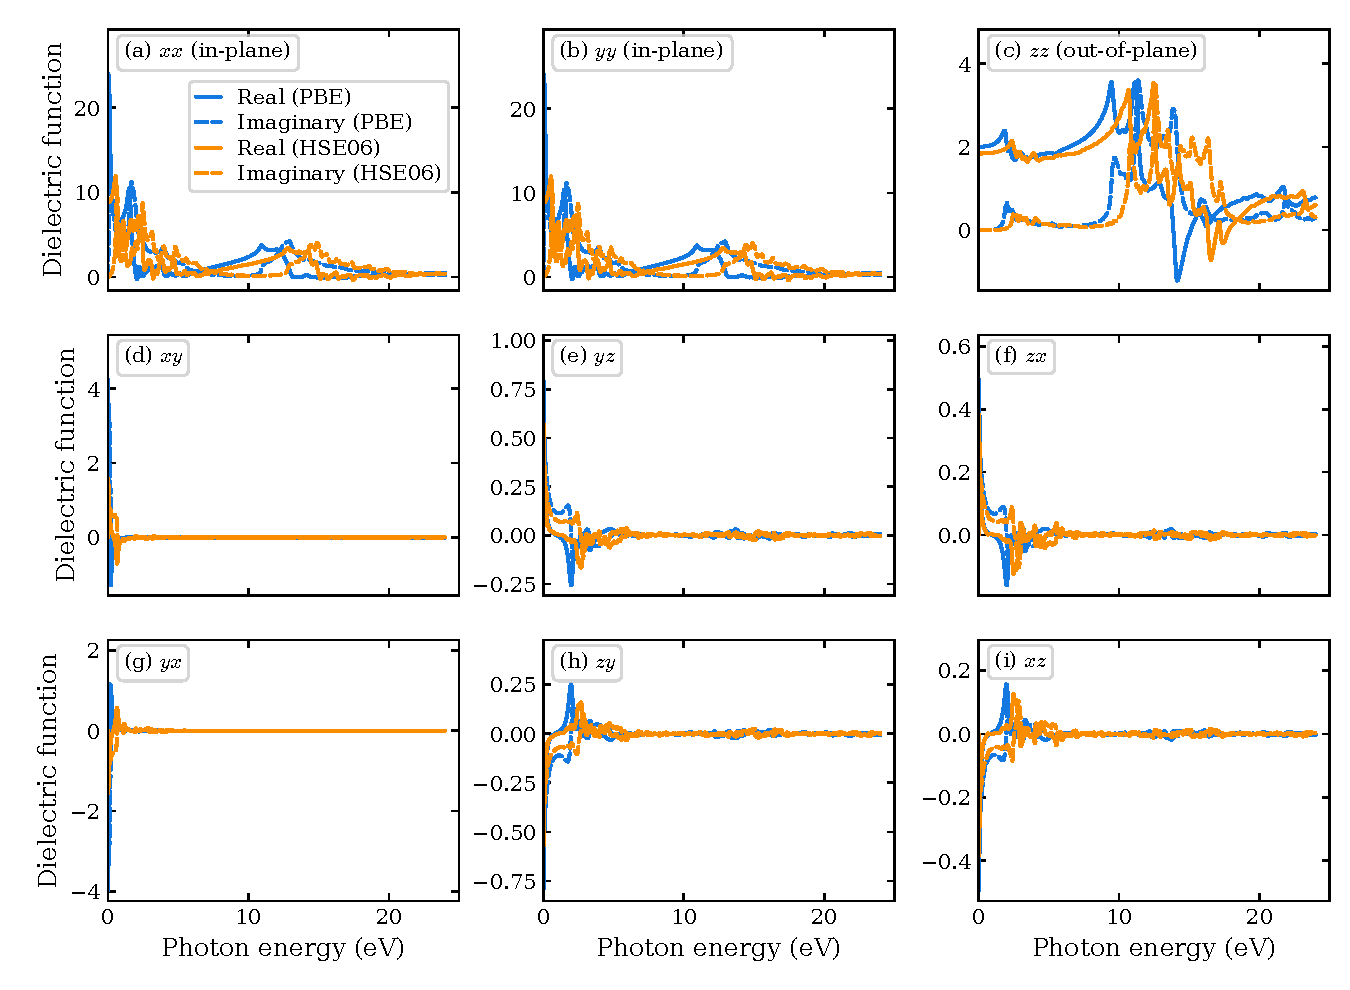
\includegraphics[width=1.00\textwidth]{figures_proj1/S1.18.pdf}
\caption[Dielectric tensor of Graphene-\ce{BC3} calculated using PBE and HSE06.]{Dimensionless dielectric tensor components of Graphene-\ce{BC3} versus photon energy $\hbar\omega$ in \unit{\electronvolt}.
From left to right, the rows show $xx,yy,zz$; $xy,yz,zx$; and $yx,zy,xz$.
The $xx$ and $yy$ directions lie within the layers, while $zz$ is perpendicular to them.
Blue and orange curves denote PBE and HSE06, respectively; solid and dashed lines denote real and imaginary parts.
The HSE06 mesh is $17\times17\times1$.
The displayed off-diagonal response is concentrated at low photon energies.
These entries are shown as exported and remain subject to the tensor-symmetry check described in the text.}
\label{S1.18}
\end{figure}

\begin{figure}[!htbp]
\centering
    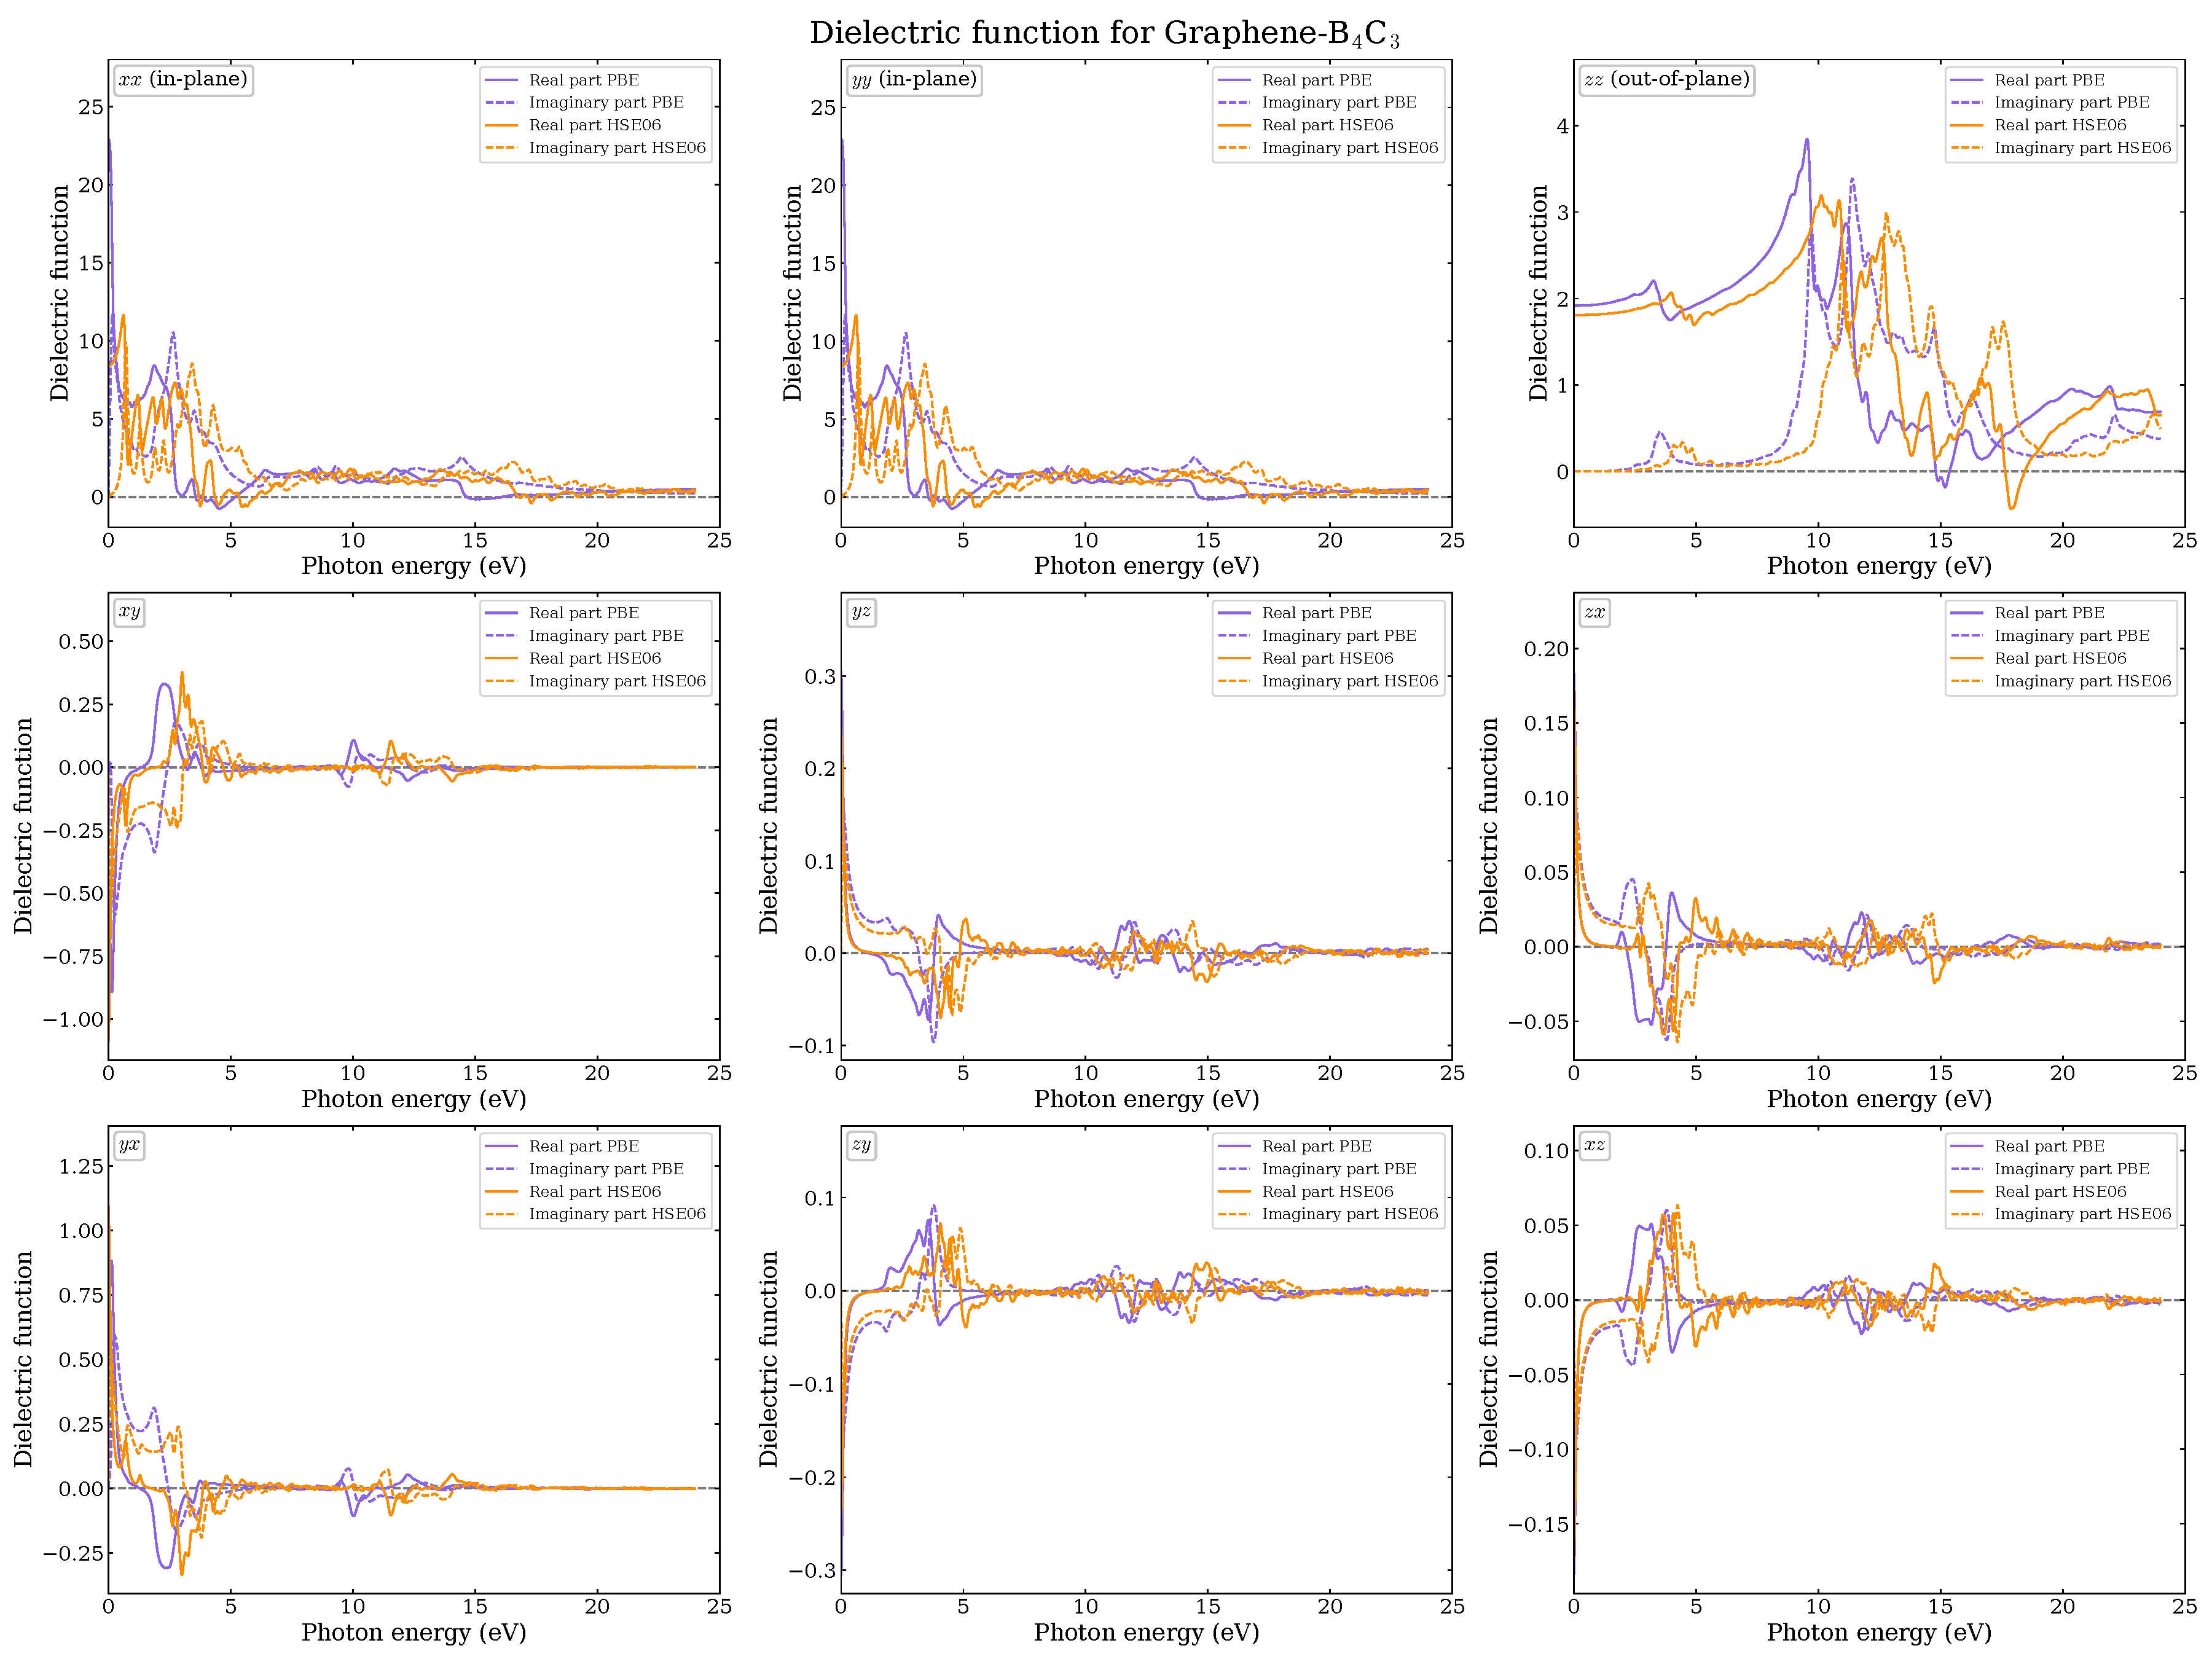
\includegraphics[width=1.00\textwidth]{figures_proj1/S1.19.pdf}
\caption[Dielectric tensor of Graphene-\ce{B4C3} calculated using PBE and HSE06.]{Dimensionless dielectric tensor components of Graphene-\ce{B4C3} versus photon energy $\hbar\omega$ in \unit{\electronvolt}.
From left to right, the rows show $xx,yy,zz$; $xy,yz,zx$; and $yx,zy,xz$.
The $xx$ and $yy$ directions lie within the layers, while $zz$ is perpendicular to them.
Purple and orange curves denote PBE and HSE06, respectively; solid and dashed lines denote real and imaginary parts.
The HSE06 mesh is $17\times17\times1$.
The displayed off-diagonal response extends beyond the low-energy region.
These entries are shown as exported and remain subject to the tensor-symmetry check described in the text.}
\label{S1.19}
\end{figure}

\begin{figure}[!htbp]
\centering
    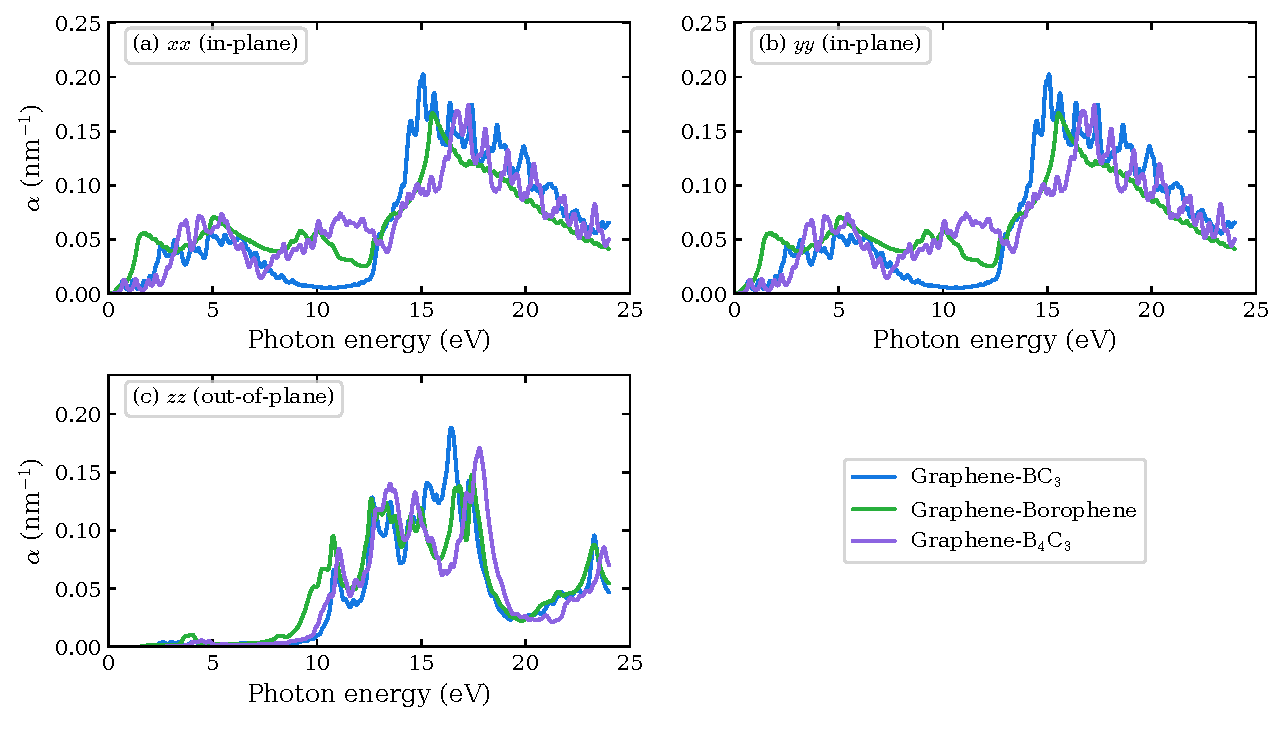
\includegraphics[width=0.80\textwidth]{figures_proj1/S1.20.pdf}
\caption[HSE06 diagonal absorption spectra of the three heterostructure bilayers.]{HSE06 absorption coefficients in \si{\per\nano\metre} for Graphene-\ce{BC3} (blue), Graphene-Borophene (green), and Graphene-\ce{B4C3} (purple).
Panels~(a), (b), and (c) show the diagonal $xx$, $yy$, and $zz$ responses, corresponding to two in-plane polarizations and the out-of-plane polarization, respectively.
All curves are solid and are plotted against photon energy $\hbar\omega$ in \unit{\electronvolt}.
The in-plane response extends into the visible region, while the strongest out-of-plane features occur in the ultraviolet region.}
\label{S1.20}
\end{figure}

\begin{figure}[!htbp]
\centering
    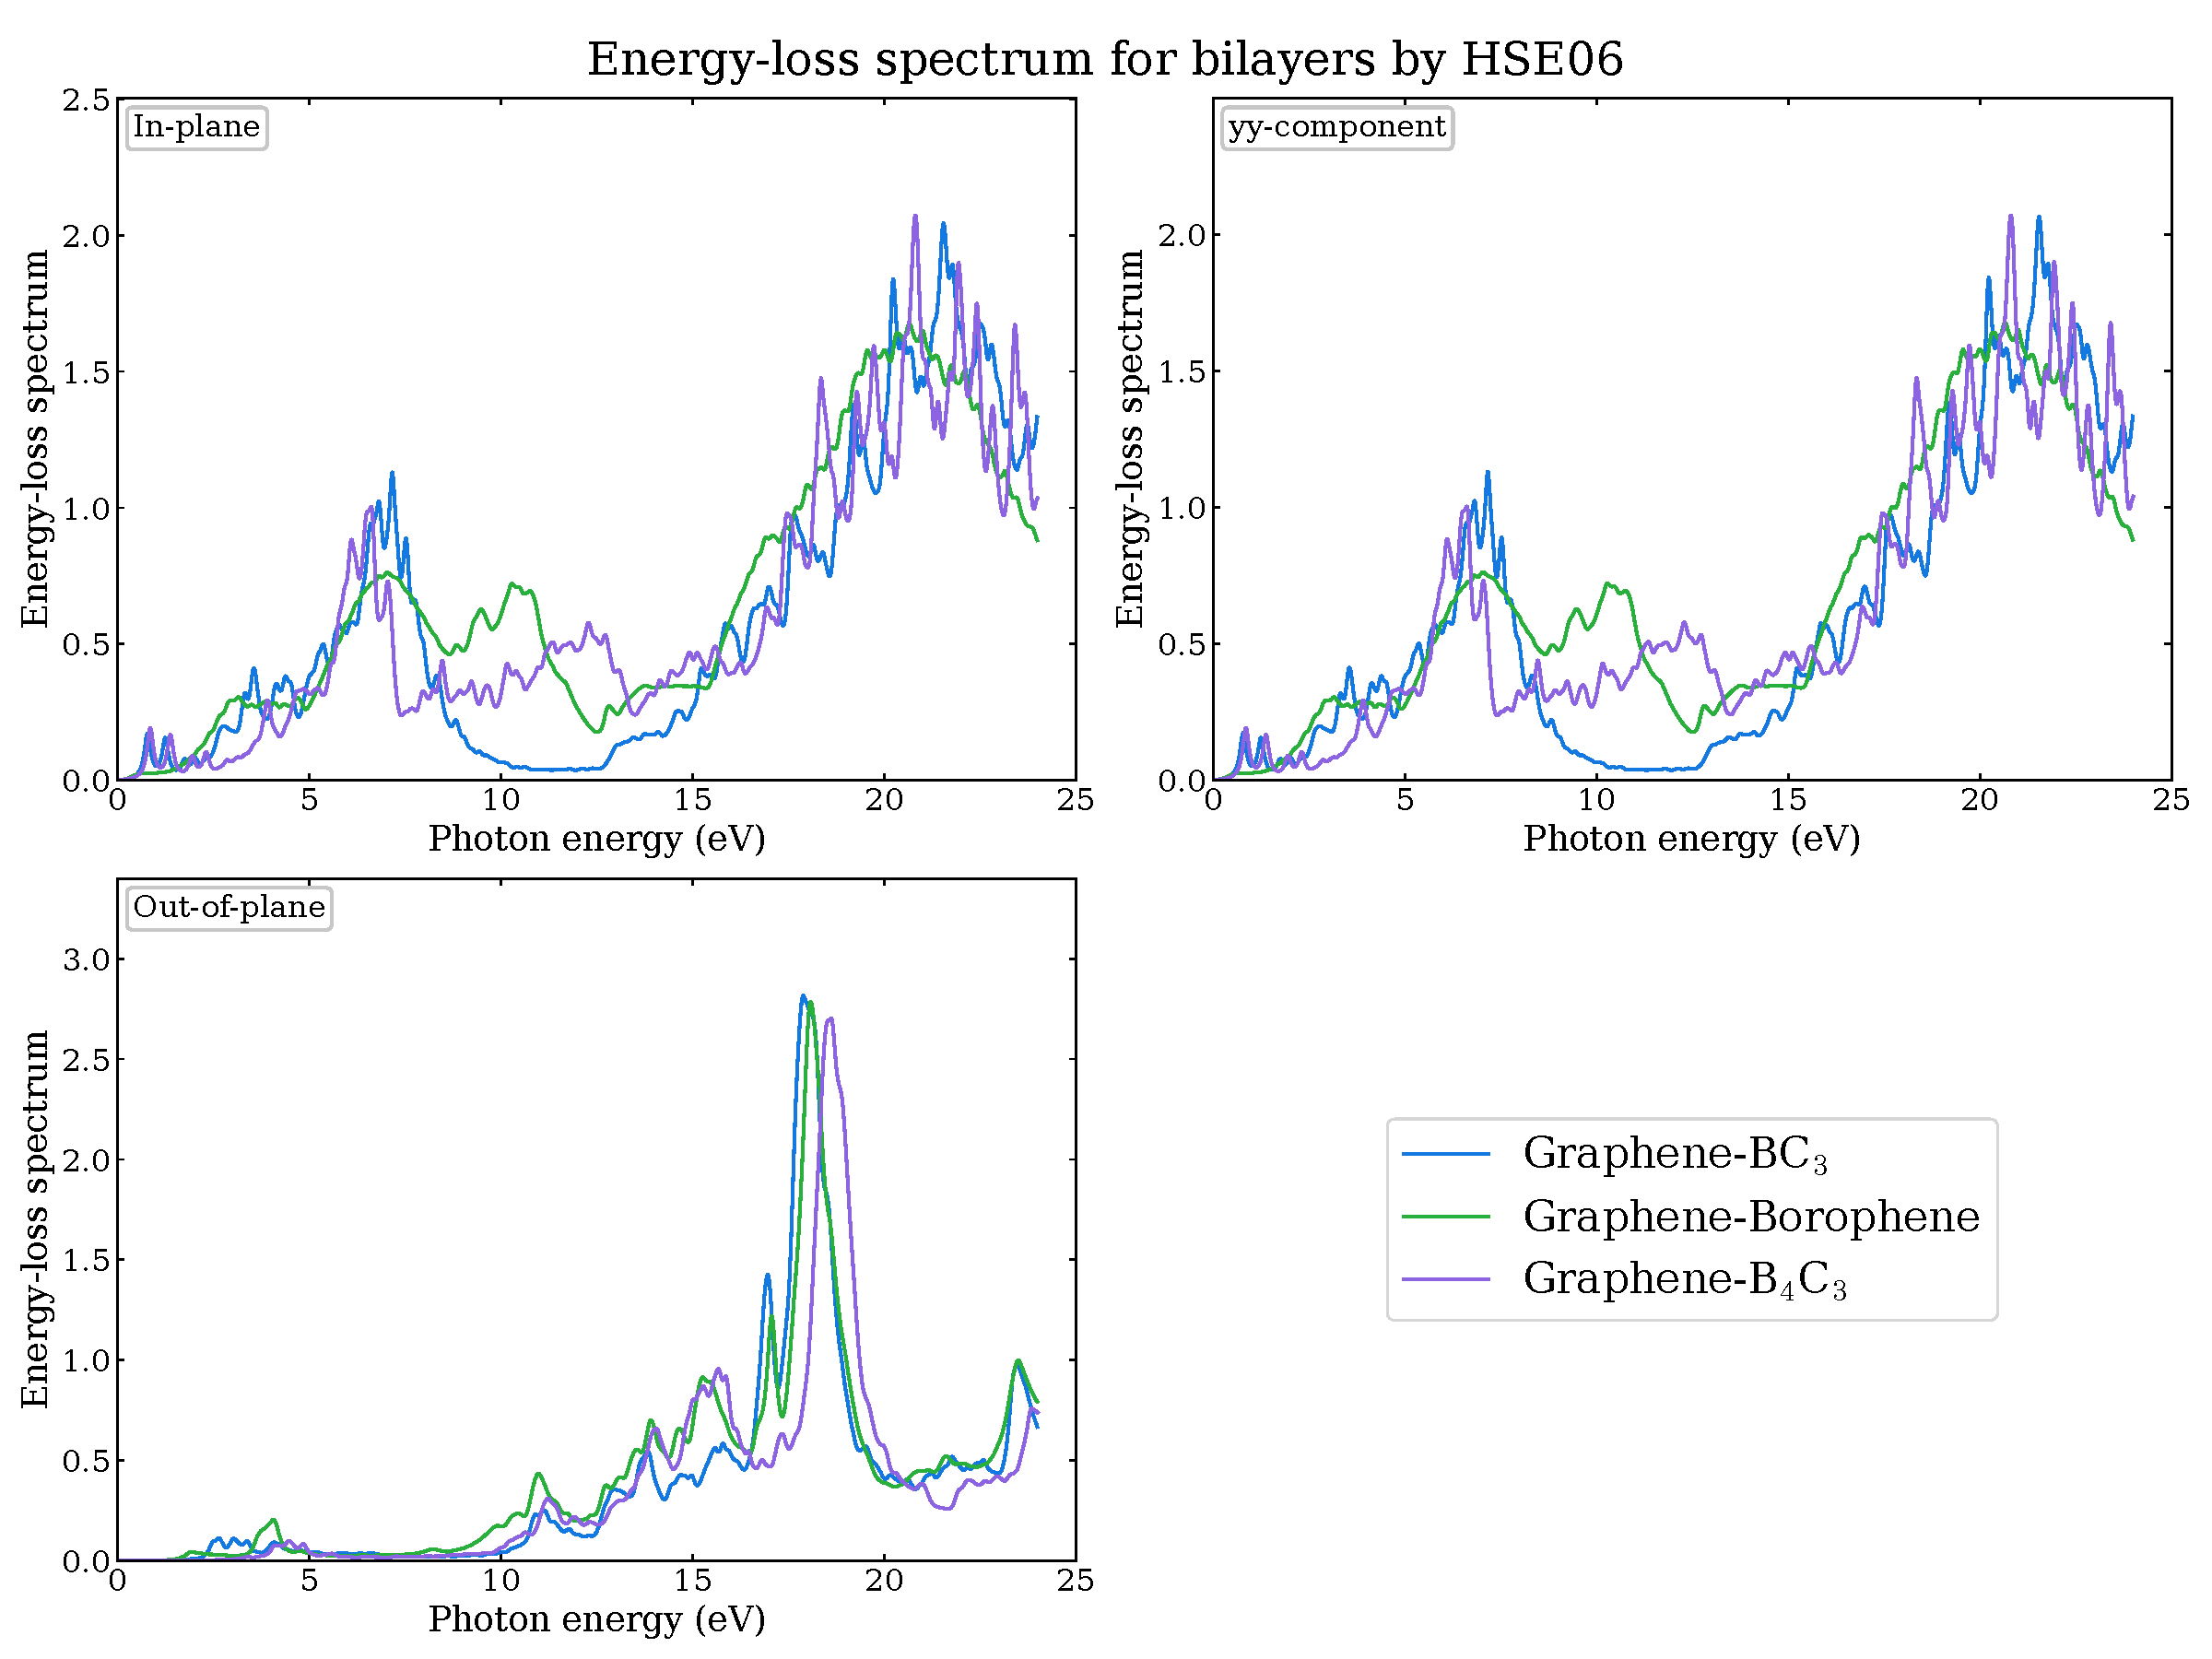
\includegraphics[width=0.80\textwidth]{figures_proj1/S1.21.pdf}
\caption[HSE06 diagonal energy-loss spectra of the three heterostructure bilayers.]{Dimensionless HSE06 energy-loss spectra of Graphene-\ce{BC3} (blue), Graphene-Borophene (green), and Graphene-\ce{B4C3} (purple).
Panels~(a), (b), and (c) show the diagonal $xx$, $yy$, and $zz$ responses, corresponding to two in-plane directions and the out-of-plane direction.
All curves are solid and are plotted against photon energy $\hbar\omega$ in \unit{\electronvolt}.
The strongest out-of-plane loss features occur around \qtyrange{17}{19}{\electronvolt}.}
\label{S1.21}
\end{figure}

\begin{figure}[!htbp]
\centering
    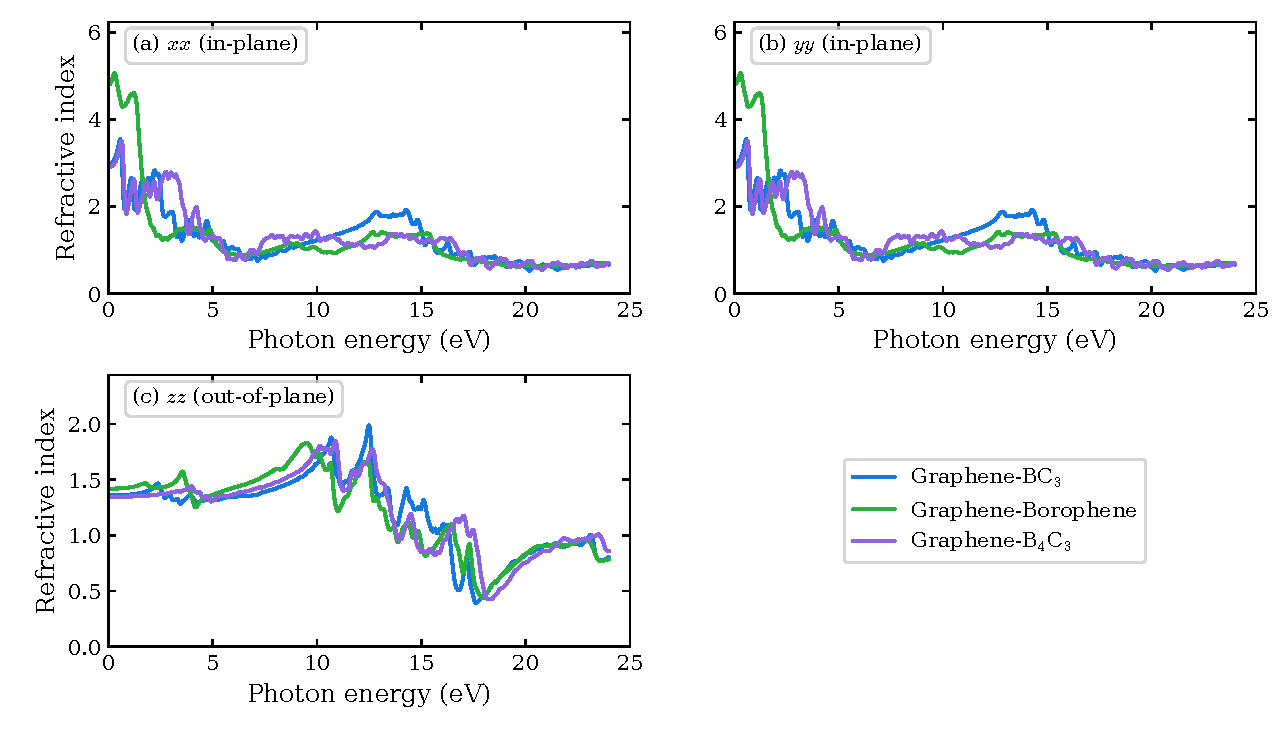
\includegraphics[width=0.80\textwidth]{figures_proj1/S1.22.pdf}
\caption[HSE06 diagonal refractive indices of the three heterostructure bilayers.]{Dimensionless HSE06 refractive indices of Graphene-\ce{BC3} (blue), Graphene-Borophene (green), and Graphene-\ce{B4C3} (purple).
Panels~(a), (b), and (c) show the diagonal $xx$, $yy$, and $zz$ responses, corresponding to two in-plane polarizations and the out-of-plane polarization.
All curves are solid and are plotted against photon energy $\hbar\omega$ in \unit{\electronvolt}.
The largest in-plane indices occur at low photon energies; the out-of-plane maxima occur at higher energies.}
\label{S1.22}
\end{figure}

\begin{figure}[!htbp]
\centering
    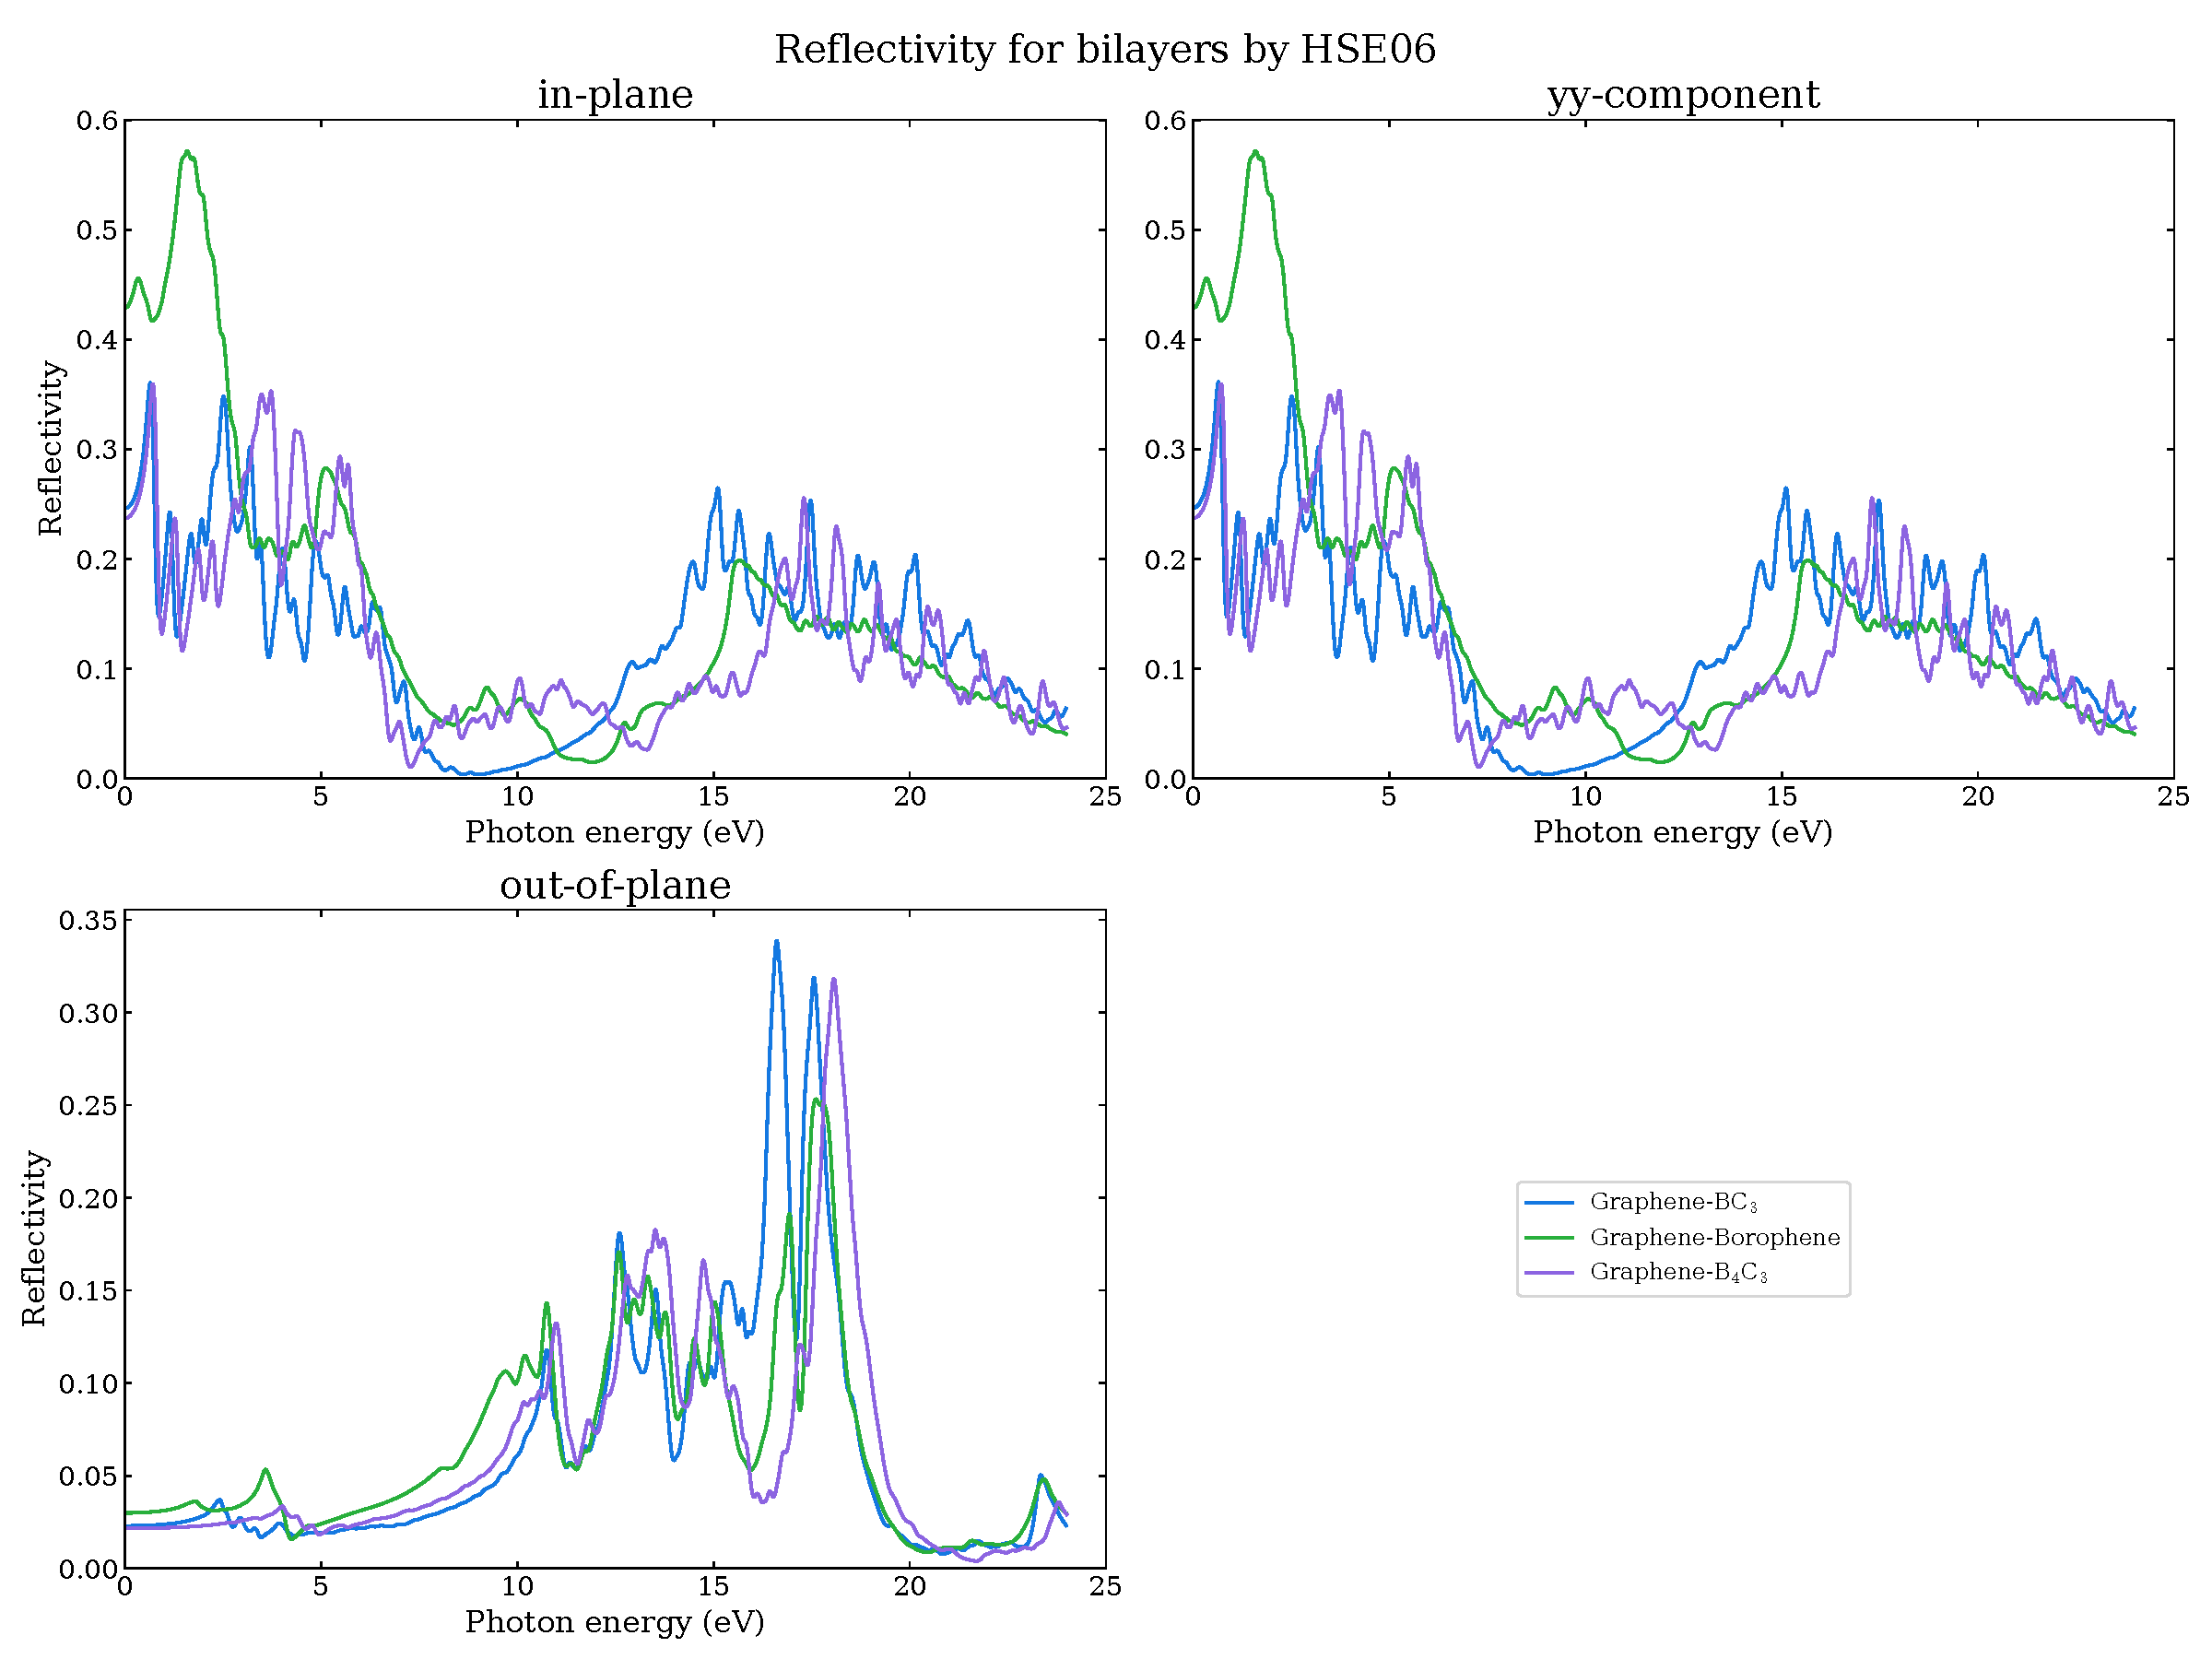
\includegraphics[width=0.80\textwidth]{figures_proj1/S1.23_correct.pdf}
\caption[HSE06 diagonal reflectivities of the three heterostructure bilayers.]{Dimensionless HSE06 reflectivities of Graphene-\ce{BC3} (blue), Graphene-Borophene (green), and Graphene-\ce{B4C3} (purple), evaluated in the principal-axis effective-medium description.
Panels~(a), (b), and (c) show the diagonal $xx$, $yy$, and $zz$ responses, corresponding to two in-plane polarizations and the out-of-plane polarization.
All curves are solid and are plotted against photon energy $\hbar\omega$ in \unit{\electronvolt}.
The out-of-plane peaks occur in the ultraviolet region.}
\label{S1.23}
\end{figure}

\begin{figure}[!htbp]
\centering
    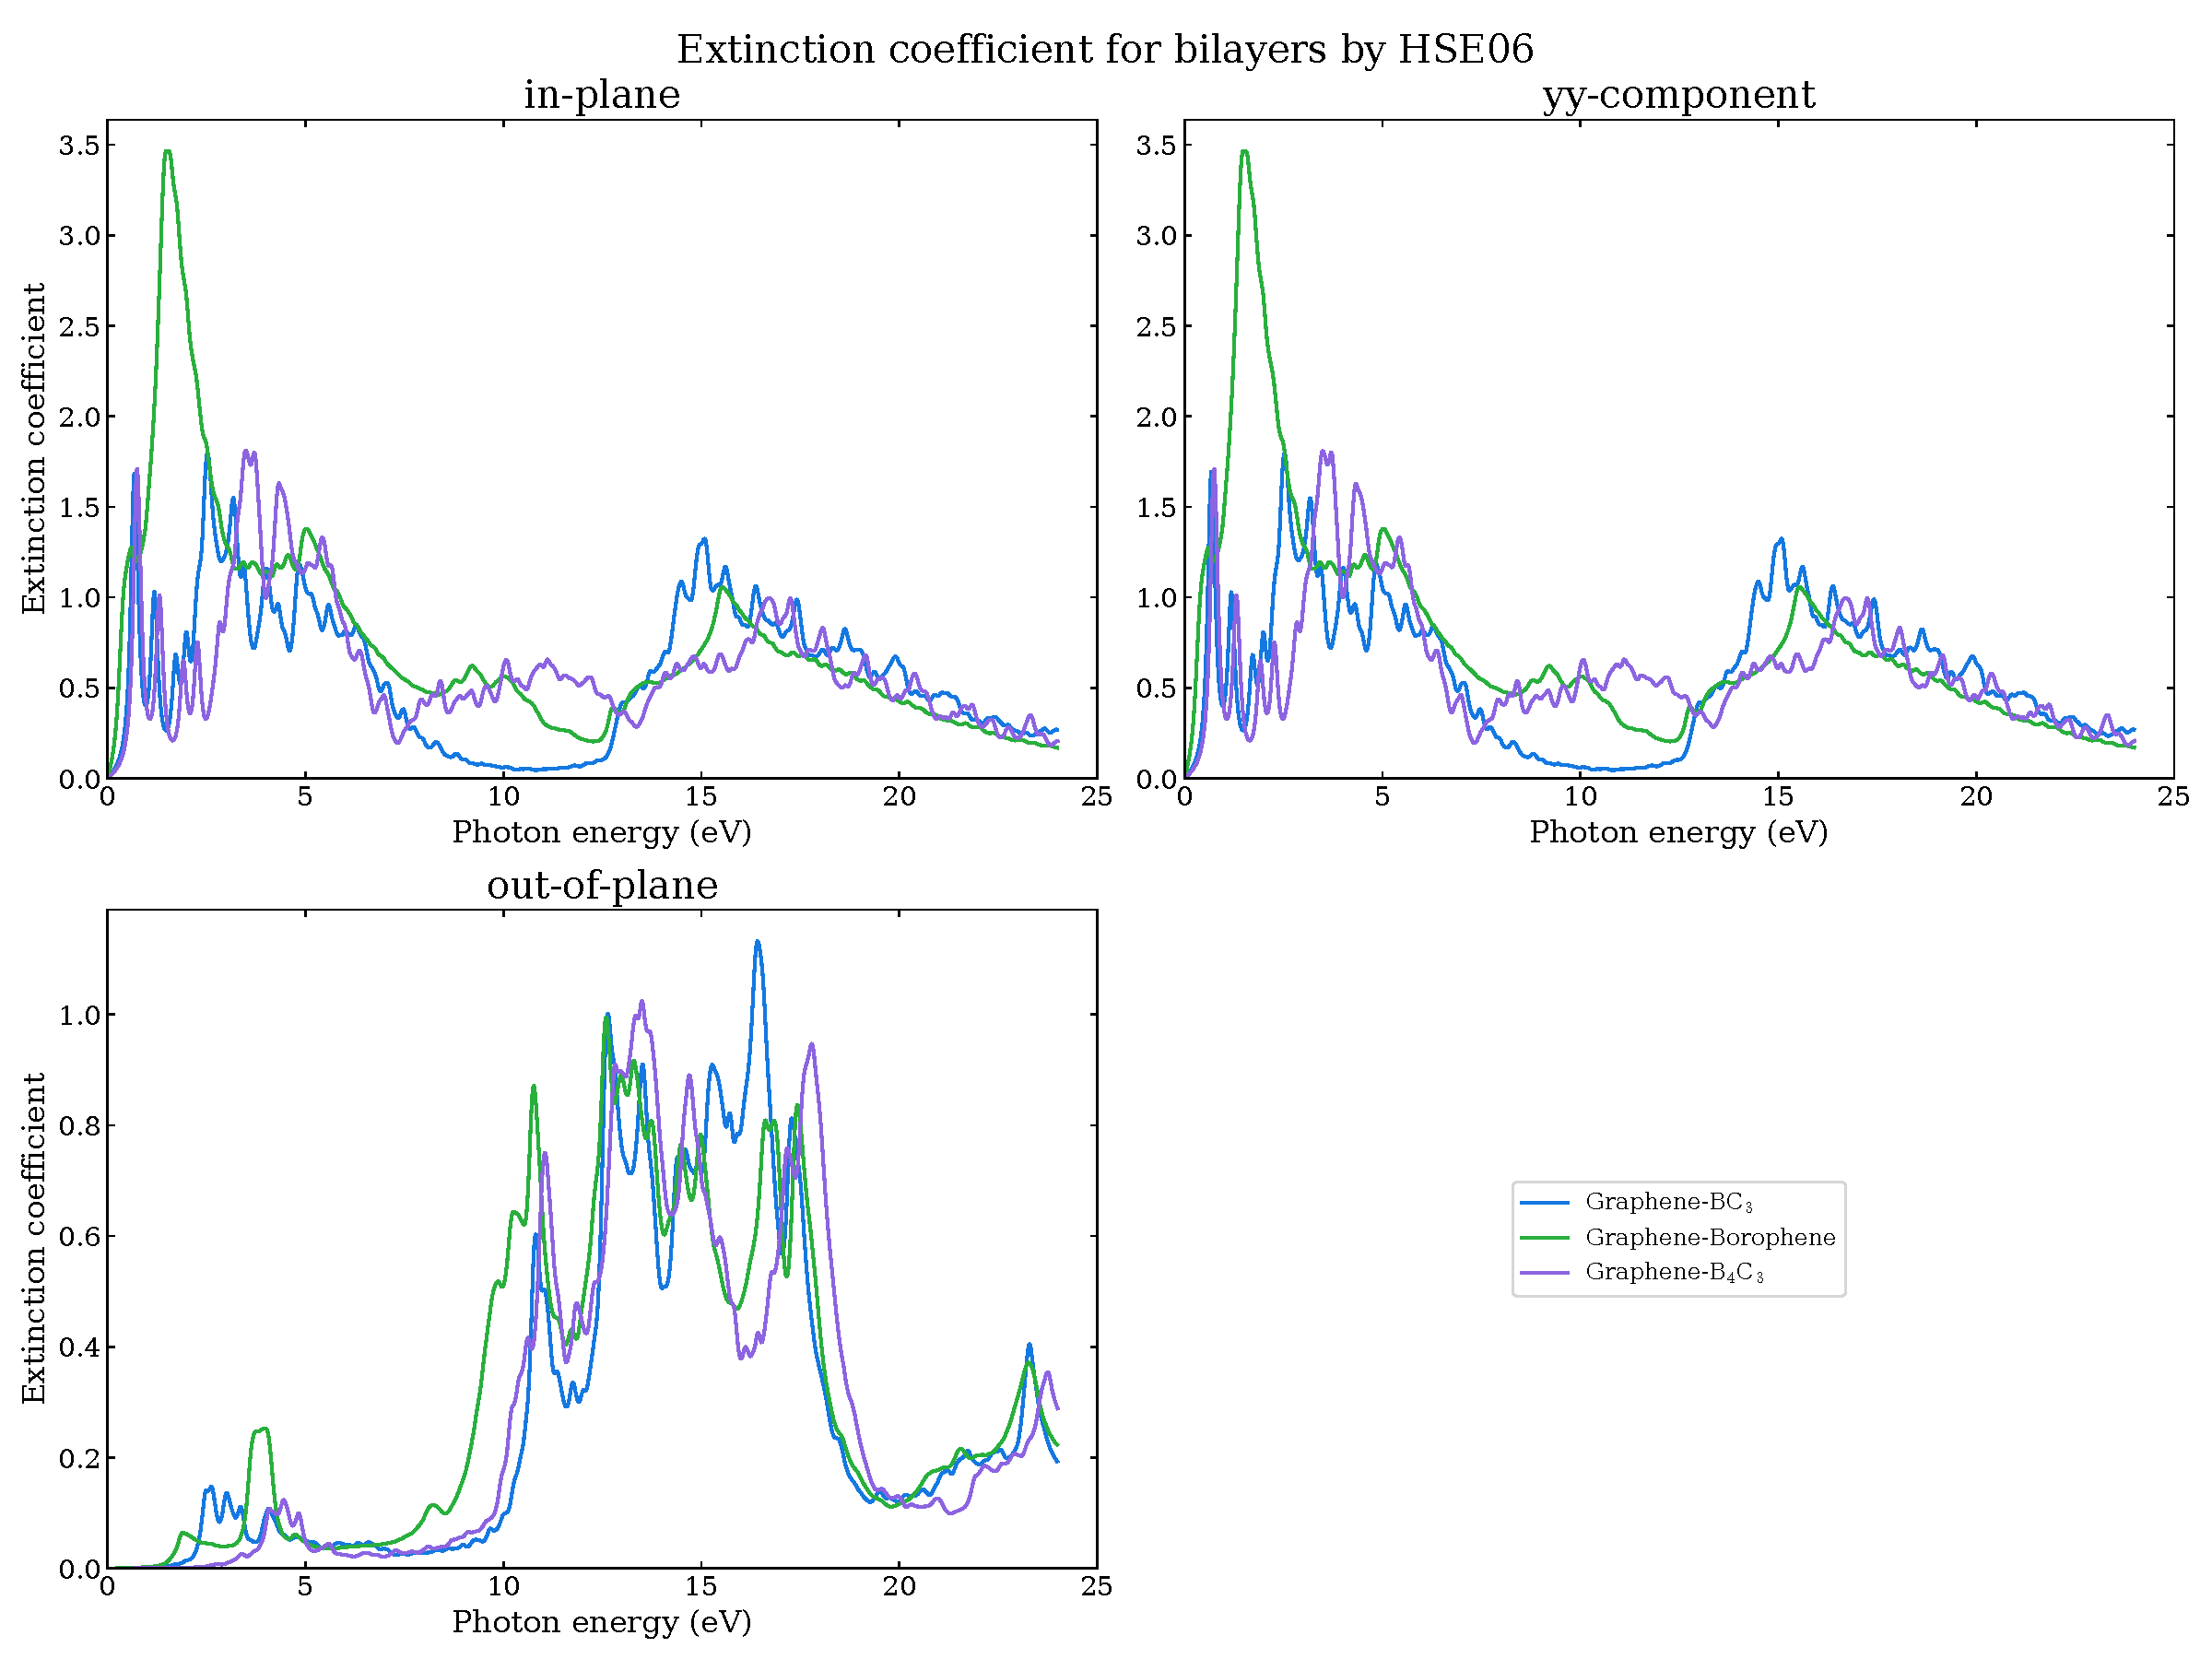
\includegraphics[width=0.80\textwidth]{figures_proj1/S1.24_correct.pdf}
\caption[HSE06 diagonal extinction coefficients of the three heterostructure bilayers.]{Dimensionless HSE06 extinction coefficients of Graphene-\ce{BC3} (blue), Graphene-Borophene (green), and Graphene-\ce{B4C3} (purple).
Panels~(a), (b), and (c) show the diagonal $xx$, $yy$, and $zz$ responses, corresponding to two in-plane polarizations and the out-of-plane polarization.
All curves are solid and are plotted against photon energy $\hbar\omega$ in \unit{\electronvolt}.
The principal in-plane features occur at lower energies than the broad out-of-plane peaks.}
\label{S1.24}
\end{figure}
